\documentclass[12pt,a4paper]{report}
\usepackage[left=3.00cm, right=2.00cm, top=2.00cm, bottom=2.00cm]{geometry}
\usepackage{vntex}
\usepackage{listings}
\usepackage{amsmath}
\usepackage{amssymb}
\usepackage{graphicx}
\usepackage{tabularx}
\usepackage{colortbl}
\usepackage{hhline}
\newcommand{\shellcmd}[1]{\\\indent\indent\texttt{\footnotesize\# #1}\\}
\newcommand{\nocontentsline}[3]{}
\newcommand{\tocless}[2]{\bgroup\let\addcontentsline=\nocontentsline#1{#2}\egroup}
\usepackage{geometry}
\geometry{
	a4paper,
	total={170mm,257mm},
	left=20mm,
	top=20mm,
	right=20mm,
	bottom=20mm,
}
\author{DSH + NAT}
\usepackage{xcolor}
\usepackage{colortbl}
\usepackage{hhline}
\setcounter{secnumdepth}{5}
\definecolor{codegreen}{rgb}{0,0.6,0}
\definecolor{codegray}{rgb}{0.5,0.5,0.5}
\definecolor{codepurple}{rgb}{0.58,0,0.82}
\definecolor{backcolour}{rgb}{0.95,0.95,0.92}

\lstdefinestyle{mystyle}{
	backgroundcolor=\color{backcolour},   
	commentstyle=\color{codegreen},
	keywordstyle=\color{magenta},
	numberstyle=\tiny\color{codegray},
	stringstyle=\color{codepurple},
	basicstyle=\ttfamily\footnotesize,
	breakatwhitespace=false,         
	breaklines=true,                 
	captionpos=b,                    
	keepspaces=true,                 
	numbers=left,                    
	numbersep=5pt,                  
	showspaces=false,                
	showstringspaces=false,
	showtabs=false,                  
	tabsize=2
}

\lstset{style=mystyle}
\usepackage{tikz}
\usetikzlibrary{calc}
\title{Đề cương chi tiết Ver 1}

\begin{document}
	\begin{titlepage}
		\begin{tikzpicture}[remember picture,overlay,inner sep=0,outer sep=0]
			\draw[blue!70!black,line width=4pt] ([xshift=-1.5cm,yshift=-2cm]current page.north east) coordinate (A)--([xshift=1.5cm,yshift=-2cm]current page.north west) coordinate(B)--([xshift=1.5cm,yshift=2cm]current page.south west) coordinate (C)--([xshift=-1.5cm,yshift=2cm]current page.south east) coordinate(D)--cycle;
			
			\draw ([yshift=0.5cm,xshift=-0.5cm]A)-- ([yshift=0.5cm,xshift=0.5cm]B)--
			([yshift=-0.5cm,xshift=0.5cm]B) --([yshift=-0.5cm,xshift=-0.5cm]B)--([yshift=0.5cm,xshift=-0.5cm]C)--([yshift=0.5cm,xshift=0.5cm]C)--([yshift=-0.5cm,xshift=0.5cm]C)-- ([yshift=-0.5cm,xshift=-0.5cm]D)--([yshift=0.5cm,xshift=-0.5cm]D)--([yshift=0.5cm,xshift=0.5cm]D)--([yshift=-0.5cm,xshift=0.5cm]A)--([yshift=-0.5cm,xshift=-0.5cm]A)--([yshift=0.5cm,xshift=-0.5cm]A);
			
			
			\draw ([yshift=-0.3cm,xshift=0.3cm]A)-- ([yshift=-0.3cm,xshift=-0.3cm]B)--
			([yshift=0.3cm,xshift=-0.3cm]B) --([yshift=0.3cm,xshift=0.3cm]B)--([yshift=-0.3cm,xshift=0.3cm]C)--([yshift=-0.3cm,xshift=-0.3cm]C)--([yshift=0.3cm,xshift=-0.3cm]C)-- ([yshift=0.3cm,xshift=0.3cm]D)--([yshift=-0.3cm,xshift=0.3cm]D)--([yshift=-0.3cm,xshift=-0.3cm]D)--([yshift=0.3cm,xshift=-0.3cm]A)--([yshift=0.3cm,xshift=0.3cm]A)--([yshift=-0.3cm,xshift=0.3cm]A);
			
		\end{tikzpicture}
		\begin{center}
			BAN CƠ YẾU CHÍNH PHỦ\\
			\textbf{HỌC VIỆN KỸ THUẬT MẬT MÃ}
		\end{center}
		\begin{figure}[h]
			\centering
			\includegraphics[width=0.25\linewidth]{"Pics/Logo HV"}
			\label{fig:logo-hv}
		\end{figure}
		
		\begin{center}
			{\Huge THỰC TẬP TỐT NGHIỆP\\}
			{\large BÁO CÁO THỰC TẬP TỐT NGHIỆP\\}
			\textbf{TRIỂN KHAI HỆ THỐNG MICROSERVICES TÍCH HỢP LIÊN TỤC}
		\end{center}
		\bigskip
		\begin{flushright}
			\large{Ngành: An toàn thông tin}
		\end{flushright}
		\begin{flushright}
			\large{Mã số: 7.48.02.02}
		\end{flushright}
		\vspace{30mm}
		\begin{flushleft}
			\textit{Sinh viên thực hiện:}\\
			\textbf{Nguyễn Anh Tuấn}\\
			Mã sinh viên: AT160258\\
			\bigskip
			\textit{Đơn vị thực tập:}\\
			\textbf{DUBE Technology}
			\bigskip\\
			\textit{Người quản lý thực tập:}\\
			\textbf{TS. Nguyễn Mạnh Thắng}\\
			Khoa An toàn thông tin - Học viện Kỹ thuật mật mã
		\end{flushleft}
		\vfill
		\begin{center}
			Hà Nội, 2023
		\end{center}
		
	\end{titlepage}
	
	\tableofcontents
	\chapter*{\centering Lời mở đầu}
	\addcontentsline{toc}{chapter}{Lời mở đầu}
	\hspace{1cm}{Đối với một sinh viên năm cuối, thực tập tốt nghiệp là một phần không thể thiếu đối tất cả. Đối với các nhà tuyển dụng, khi tuyển dụng, họ sẽ thường có những yêu cầu nhất định như kinh nghiệm làm việc, bằng cấp, kĩ năng trong công việc,... Việc này là những thứ khó có thể có đối với các sinh viên trong giai đoạn cuối cùng của cấp bậc đại học. Do đó, thực tập tốt nghiệp là một bước đệm quan trọng không thể thiếu đối với những sinh viên năm cuối, đang trong giai đoạn chuẩn bị bước vào con đường sự nghiệp sau nhiều năm học hành.\\}
	
	\hspace{0.3cm}{Trong thực tập tốt nghiệp, sinh viên sẽ được hướng dẫn bởi các người hướng dẫn dày dặn kinh nghiệm trong một phòng ban. Người này sẽ chịu trách nhiệm giám sát, kiểm tra, hỗ trợ sinh viên trong những bước đầu trong ngành. Sinh viên sẽ cần phải học các kĩ năng mình còn thiếu, thực hành các bài tập do người hướng dẫn đề ra. Sau đấy, sinh viên sẽ cần phải thuyết trình lại những thứ mình đã đạt được và những thứ chưa đạt được ở bài tập này cho người hướng dẫn, để họ có thể nắm bắt được tình hình cụ thể.\\}
	
	\hspace{0.3cm}{Sau quá trình đấy, rơi vào khoảng 3 tháng làm việc, sinh viên sẽ có một lượng kiến thức nhất định, một số kinh nghiệm nhất định để có thể tiếp tục bước đi trong ngành mình theo đuổi. Có thể sinh viên sẽ được tiếp tục làm việc tại nơi mà sinh viên đăng kí thực tập, hoặc sinh viên có thể cảm thấy môi trường tại đấy không phù hợp và có thể chuyển sang môi trường làm việc khác để có trải nghiệm riêng mình.\\}
	
	\hspace{0.3cm}{Về cơ bản, thực tập tốt nghiệp sẽ giúp sinh viên hiểu rõ hơn về sở thích, định hướng của mình trong tương lai. Thực tập tốt nghiệp sẽ mang lại một trải nghiệm mới mẻ cho sinh viên, một trong những thứ giúp sinh viên xác minh được định hướng rõ ràng của mình.\\}
	
	\chapter{Giới thiệu chung về Cơ sở thực tập}
	\section{Loại hình tổ chức/doanh nghiệp}
	
	\hspace{1cm}{Kubernetes hoặc k8s là một nền tảng mã nguồn mở giúp tự động hóa việc quản lý, mở rộng và triển khai ứng dụng dưới dạng container. Kubernetes còn được gọi là Container Orchestration Engine (hiểu nôm na là công cụ điều phối container). Kubernetes loại bỏ rất nhiều các quy trình thủ công liên quan đến việc triển khai và mở rộng các containerized applications. Các ứng dụng có thể khác nhau về kích thước: từ 1 cho đến hàng nghìn server. Với Kubernetes chúng ta có thể phát triển application một cách linh hoạt và đáng tin cậy. \\}
	
	\hspace{0.3cm}{Trách nhiệm chính của Kubernetes là container orchestration (dịch ra có nghĩa điều phối container). Kubernetes đảm bảo rằng tất cả container được lên lịch chạy trên các cụm server (cluster) (server ở đây có thể là physical machine hoặc virtual machine). Ngoài ra, Kubernetes còn có chức năng theo dõi hoạt động của từng container, mở rộng các containers và quản lý tình trạng của các containers theo thời gian. Khi một container nào đó gặp trục trặc, dừng hoạt động thì Kubernetes sẽ thay thế container đó. \\}
	
	\hspace{0.3cm}{Kubernetes ban đầu được các kỹ sư Google phát triển vào năm 2014. Và Google cũng là một trong những cái tên tiên phong đóng góp cho công cuộc phát triển công nghệ Linux container. \\}
	
	\hspace{0.3cm}{Kubernetes ban đầu được các kỹ sư Google phát triển vào năm 2014. Và Google cũng là một trong những cái tên tiên phong đóng góp cho công cuộc phát triển công nghệ Linux container. \\}
	
	\hspace{0.3cm}{Red Hat là một trong những công ty đầu tiên hợp tác với Google trong dự án Kubernetes trước khi Kubernetes được ra mắt, và trở thành nhà tài trợ lớn thứ 2 cho dự án ngay từ những ngày đầu. Và Google đã tặng lại dự án Kubernetes cho Cloud Native Computing Foundation (CNCF - thành lập năm 2015). Kubernetes đã trở thành một project của tổ chức này cho đến thời điểm hiện tại. Năm 2018, Kubernetes Project đạt vị trí thứ 9 về số lượt commit trên Github.}
	\subsection{Khái quát quá trình hình thành và phát triển}
	
	\hspace{1cm}{Khi bạn triển khai Kubernetes, bạn sẽ nhận được một Cluster (cụm máy chủ). \\}
	
	\hspace{0.3cm}{Một Cluster Kubernetes bao gồm một tập hợp các máy worker, được gọi là Node, chạy các ứng dụng được đóng gói. Mỗi Cluster có ít nhất một Node. \\}
	
	\hspace{0.3cm}{(Các) Node lưu trữ các Pod - Một nhóm gồm một hoặc nhiều containers được triển khai cho single Node, nhóm này chia sẻ chung không gian lưu trữ, IP address, hostname, và những nguồn khác. \\}
	
	\hspace{0.3cm}{Các Control Plane quản lý các Node và các Pod trong Cluster. Trong môi trường production, Control Plane thường chạy trên nhiều máy tính và một Cluster thường chạy nhiều Node, mang lại khả năng chịu lỗi và tính sẵn sàng cao. \\}
	
	\hspace{0.3cm}{Trên đây là sơ đồ của một cụm Kubernetes với tất cả các thành phần được gắn với nhau.}
	
	\begin{figure}
		\centering
		\includegraphics[width=1\textwidth]{"Pics/components-of-kubernetes"}
		\caption{\label{fig:components-of-kubernetes} Sơ đồ của một cụm Kubernetes.}
		\label{fig:components-of-kubernetes}
	\end{figure}
	
	\subsubsection{Các thành phần Control Plane (Master)}
	
	\hspace{1cm}{Các thành phần Control Plane đưa ra các quyết định chung về Cluster (ví dụ: lập lịch), cũng như phát hiện và phản hồi các sự kiện của Cluster. \\}
	
	\hspace{0.3cm}{Các thành phần Control Plane có thể được chạy trên bất kỳ máy nào trong Cluster. Tuy nhiên, để đơn giản, thiết lập tập lệnh thường khởi động tất cả các thành phần Control Plane trên cùng một máy và không chạy các container của người dùng trên máy này. \\}
	
	\hspace{0.3cm}{Đối với cluster nhỏ , Master có thể chạy trên một Node, nhưng trong một cluster lớn, để đảm bảo tính khả dụng (trong tiếng anh là High-Availability) thì Master có thể được chạy trên nhiều Node. (Tính khả dụng có nghĩa là Khi mà một Node trong cluster dừng hoạt động thì hệ thống vẫn duy trì như không có gì xảy ra). Master sẽ bao gồm 5 thành phần chính sau:}
	
	\begin{itemize}
	\item \textbf{kube-apiserver:}
	\smallskip
	\subitem
	API Server là một thành phần của Control Plane. Đúng theo tên gọi, đây chính là server cung cấp REST API cho Kubernetes Cluster. Nó có nhiệm vụ đặt Pod vào Node, đồng bộ hoá thông tin của Pod bằng REST API tiếp nhận cài đặt, xác thực và thiết lập cho các objects pod/service/replicationController.
	
	\item \textbf{Etcd:}
	\smallskip
	\subitem
	Etcd là Kho lưu trữ giá trị khóa nhất quán và có tính khả dụng cao được sử dụng làm kho dự phòng để lưu trữ toàn bộ cấu hình, trạng thái và metadata của Kubernetes Cluster.
	\smallskip
	\subitem Trong các cluster nhỏ, Etcd có thể chạy trên cùng một Node với các thành phần khác. Nhưng trong các cluster lớn, Etcd có thể chạy dự phòng trên nhiều Node để đảm bảo tính khả dụng của toàn hệ thống. Nếu cụm Kubernetes của bạn sử dụng Etcd làm nơi lưu trữ sao lưu, hãy đảm bảo rằng bạn có kế hoạch sao lưu cho những dữ liệu đó.
	
	\item \textbf{kube-controller-manager:}
	\smallskip
	\subitem
	Kube Controller Manage một tập hợp các controller khác nhau để chạy các bộ điều khiển quy trình theo dõi các cập nhật trạng thái của Kubernetes Cluster thông qua API và thực hiện các thay đổi đối với Cluster sao cho phù hợp. 
	\smallskip
	\subitem Về mặt logic, mỗi bộ điều khiển là một quy trình riêng biệt, nhưng để giảm độ phức tạp, tất cả chúng đều được biên dịch thành một tệp nhị phân duy nhất và chạy trong một quy trình duy nhất.
	\smallskip
	\subitem Một số loại bộ điều khiển có thể kể đến:
	\begin{itemize}
		\item Node controller: Chịu trách nhiệm thông báo và phản hồi khi các Node gặp sự cố.

		
		\item \textbf{Etcd:}
		\subitem
		Etcd là Kho lưu trữ giá trị khóa nhất quán và có tính khả dụng cao được sử dụng làm kho dự phòng để lưu trữ toàn bộ cấu hình, trạng thái và metadata của Kubernetes Cluster.
		
		\hspace{0.8cm}{Trong các cluster nhỏ, Etcd có thể chạy trên cùng một Node với các thành phần khác. Nhưng trong các cluster lớn, Etcd có thể chạy dự phòng trên nhiều Node để đảm bảo tính khả dụng của toàn hệ thống. Nếu cụm Kubernetes của bạn sử dụng Etcd làm nơi lưu trữ sao lưu, hãy đảm bảo rằng bạn có kế hoạch sao lưu cho những dữ liệu đó.}
		

		\item Service Account \& Token controllers: Tạo tài khoản mặc định và mã thông báo truy cập API cho không gian tên mới.
	\end{itemize}

	\item \textbf{cloud-controller-manager:}
	\smallskip
	\subitem
	Là một tập hợp các logic dành riêng cho đám mây (GCP, AWS, Azure) cho phép bạn liên kết Kubernetes Cluster với API của nhà cung cấp đám mây và tách các thành phần tương tác với nền tảng đám mây đó khỏi các thành phần chỉ tương tác với cụm của bạn. Cloud-controller-manager chỉ chạy các bộ điều khiển dành riêng cho nhà cung cấp dịch vụ đám mây của bạn. Nếu bạn đang chạy Kubernetes tại cơ sở của riêng mình hoặc trong môi trường học tập bên trong PC của riêng bạn, cụm không có trình quản lý bộ điều khiển đám mây.
	\smallskip
	\subitem Cũng như với kube-controller-manager, cloud-controller-manager kết hợp một số vòng điều khiển độc lập về mặt logic thành một tệp nhị phân duy nhất mà bạn chạy như một quy trình duy nhất. Bạn có thể chia tỷ lệ theo chiều ngang (chạy nhiều hơn một bản sao) để cải thiện hiệu suất hoặc để giúp tăng khả năng chịu lỗi.
	\smallskip
	\subitem Các bộ điều khiển sau có thể có các phần phụ thuộc của nhà cung cấp dịch vụ đám mây:
	\begin{itemize}
	\item Node controller: Để kiểm tra nhà cung cấp đám mây để xác định xem một Node đã bị xóa trong đám mây sau khi nó ngừng phản hồi hay chưa.
	
	\item Route controller: Để thiết lập định tuyến trong cơ sở hạ tầng đám mây cơ bản.
	
	\item Service controller: Để tạo, cập nhật và xóa bộ cân bằng tải của nhà cung cấp dịch vụ đám mây.
	\end{itemize}
	
	\item \textbf{kube-scheduler:}
	\smallskip
	\subitem
	Sử dụng Kubernetes API để tìm, theo dõi các Pod chưa được lên lịch hoặc mới được tạo nhưng không được chỉ định Node. Sau đó, scheduler sẽ đặt các Pod này vào các Node dựa trên tài nguyên và các ràng buộc khác được định nghĩa trong manifest file của Pod. Scheduler sẽ cố gắng đảm bảo rằng các Pod của cùng một application sẽ được phân phối trên các Node khác nhau để đảm bảo tính khả dụng.
	\smallskip
	\subitem Các yếu tố được tính đến để đưa ra quyết định lập lịch bao gồm: yêu cầu tài nguyên cá nhân và tập thể, các ràng buộc về phần cứng / phần mềm / chính sách, thông số kỹ thuật về mối quan hệ và chống mối quan hệ, vị trí dữ liệu, can thiệp giữa khối lượng công việc và thời hạn.
	\end{itemize}


	\subsubsection{Các thành phần Worker}
	
	\hspace{1cm}{Có nhiệm vụ xử lý khối lượng công việc của application trong cluster, duy trì các nhóm đang chạy và cung cấp môi trường runtime cho Kubernetes. Worker sẽ bao gồm 3 thành phần chính sau:}
	\begin{itemize}
		\item \textbf{kubelet:}
		\smallskip
		\subitem
		Kubelet chạy trên mỗi Worker Node. Nó đảm bảo rằng các container đang chạy trong một Pod và có trách nhiệm giám sát giao tiếp với master node và quản lý các Pod. Kubelet sử dụng CRI (Container Runtime Interface - Giao diện thời gian chạy vùng chứa) để giao tiếp với container runtime trên cùng một Node đó. Kubelet không quản lý các vùng chứa không được tạo bởi Kubernetes.
		
		\item \textbf{kube-proxy:}
		\smallskip
		\subitem
		Là một proxy mạng chạy trên mỗi Node trong Cluster. Nó có trách nhiệm quản lý, duy trì các quy tắc mạng trên mỗi Node. Các quy tắc mạng này cho phép giao tiếp mạng với Pod của bạn từ các phiên mạng bên trong hoặc bên ngoài Cluster. kube-proxy sử dụng lớp lọc gói của hệ điều hành nếu có và nó có sẵn. Nếu không, kube-proxy sẽ tự chuyển tiếp lưu lượng.
		
		\item \textbf{Container Runtime:}
		\smallskip
		\subitem
		Là phần mềm chịu trách nhiệm chạy các container. Kubernetes hỗ trợ một số container runtime như: Docker, containerd, CRI-O và bất kỳ triển khai nào của Kubernetes CRI (Container Runtime Interface).
	\end{itemize}
	
	\section{Khái quát quá trình hình thành và phát triển}
	
	\subsection{Node}
	
		\hspace{1cm}{Kubernetes chạy khối lượng công việc bằng cách đặt các container vào các Pod để chạy trên các Node. Một Node có thể là một máy ảo hoặc vật lý, tùy thuộc vào cụm. Mỗi Node được quản lý bởi control plane và chứa các dịch vụ cần thiết để chạy các Pod.\\}
	
	\hspace{0.3cm}{Thông thường, có một số Node trong một cụm; trong môi trường học tập hoặc tài nguyên hạn chế, có thể chỉ có một Node.\\}
	
	\hspace{0.3cm}{Các thành phần trên một Node bao gồm kubelet, container runtime (là thành phần giúp chạy các ứng dụng dưới dạng container), và kube-proxy.}
	
	\begin{figure}[h]
		\centering
		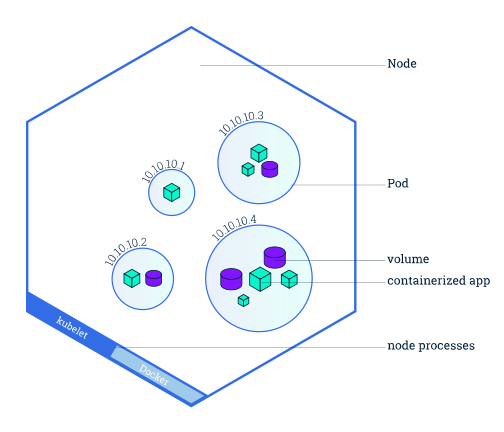
\includegraphics[width=0.7\linewidth]{Pics/nodes}
		\caption{\label{fig:nodes} Cấu tạo của Nodes.}
		\label{fig:nodes}
	\end{figure}
	
	\subsubsection{Quản lý}
	
	\hspace{1cm}{Có hai cách chính để thêm các Node vào máy chủ API:}
	
	\begin{enumerate}
		\item Kubelet trên một Node tự đăng ký vào control plane
		\item Thêm một đối tượng Node theo cách thủ công\\
	\end{enumerate}
	
	\hspace{0.3cm}{Sau khi bạn tạo một đối tượng Node hoặc kubelet trên Node tự đăng ký, control plane sẽ kiểm tra xem đối tượng Node mới có hợp lệ hay không. Ví dụ: nếu bạn cố gắng tạo một Node từ tệp kê khai JSON sau:\\}
	
	\begin{lstlisting}[language=Bash]
		{
			"kind": "Node",
			"apiVersion": "v1",
			"metadata": {
				"name": "10.240.79.157",
				"labels": {
					"name": "my-first-k8s-node"
				}
			}
		}
	\end{lstlisting}
	\smallskip
	
	\hspace{0.3cm}{Kubernetes tạo một đối tượng Node nội bộ. Kubernetes kiểm tra xem kubelet đã đăng ký với máy chủ API khớp với trường \texttt{metadata.name} của ứng dụng Node. Nếu Node hoạt động tốt (tức là tất cả các dịch vụ cần thiết đang chạy), thì Node đó đủ điều kiện để chạy Pod. Nếu không, Node đó sẽ bị bỏ qua đối với mọi hoạt động của cụm cho đến khi nó hoạt động bình thường.\\}
	
	\hspace{0.3cm}{Tên của một đối tượng Node phải là một tên miền phụ DNS hợp lệ.}
	
	\begin{itemize}
		\item \textbf{Tính duy nhất của tên Node}
		\smallskip
		\subitem Tên xác định một Node. Hai Node không thể có cùng tên cùng một lúc. Kubernetes cũng giả định rằng một tài nguyên có cùng tên là cùng một đối tượng. Trong trường hợp một Node, người ta mặc nhiên cho rằng một thể hiện sử dụng cùng tên sẽ có cùng trạng thái (ví dụ: cài đặt mạng, nội dung đĩa gốc) và các thuộc tính như nhãn Node. Điều này có thể dẫn đến sự không nhất quán nếu một phiên bản được sửa đổi mà không thay đổi tên của nó. Nếu Node cần được thay thế hoặc cập nhật đáng kể, đối tượng Node hiện có cần được xóa khỏi máy chủ API trước và thêm lại sau khi cập nhật.
		\smallskip
		\item \textbf{Tự đăng ký Node}
		\smallskip
		\subitem Khi cờ kubelet \texttt{--register-node} là \texttt{true} (mặc định), kubelet sẽ cố gắng tự đăng ký với máy chủ API. Đây là mẫu ưa thích, được sử dụng bởi hầu hết các bản phân phối.
		\smallskip
		\subitem Để tự đăng ký, kubelet được bắt đầu với các tùy chọn sau:
		
		\begin{itemize}
			\item \texttt{-kubeconfig} Đường dẫn đến thông tin đăng nhập để tự xác thực với máy chủ API.
			\item \texttt{-cloud-provider} Nói chuyện với một nhà cung cấp đám mây để đọc siêu dữ liệu về chính nó.
			\item \texttt{-register-node} Tự động đăng ký với máy chủ API.
			\item \texttt{-register-with-taints} Đăng ký Node với danh sách Taints đã cho (phân cách bằng dấu phẩy \texttt{<key>=<value>:<effect>}).
			
			No-op nếu \texttt{register-node} là sai.
			
			\item \texttt{-node-ip} Địa chỉ IP của Node.
			\item \texttt{-node-labels} - nhãn để thêm khi đăng ký Node trong cụm.
			\item \texttt{-node-status-update-frequency} Chỉ định tần suất kubelet đăng trạng thái Node của nó lên máy chủ API.
		\end{itemize}
		\smallskip
		\item \textbf{Quản lý Node thủ công}
		\smallskip
		\subitem Có thể tạo và sửa đổi các đối tượng Node bằng cách sử dụng kubectl.
		\smallskip
		\subitem Khi muốn tạo các đối tượng Node theo cách thủ công, hãy đặt cờ kubelet     \texttt{--register-node=false}.
		\smallskip
		\subitem Có thể sửa đổi các đối tượng Node bất kể cài đặt của \texttt{--register-node}. Ví dụ: bạn có thể đặt nhãn trên một Node hiện có hoặc đánh dấu Node đó là không thể lập lịch trình.
		\smallskip
		\subitem Có thể sử dụng nhãn trên Node kết hợp với bộ chọn Node trên Pod để kiểm soát việc lên lịch. Ví dụ: bạn có thể hạn chế một Pod chỉ đủ điều kiện chạy trên một tập hợp con các Nod có sẵn.
		\smallskip
		\subitem Việc đánh dấu một Node là không thể lập lịch trình sẽ ngăn bộ lập lịch đặt các Pod mới vào Node đó nhưng không ảnh hưởng đến các Pod hiện có trên Node. Điều này hữu ích như một bước chuẩn bị trước khi khởi động lại Node hoặc bảo trì khác.
		\subitem Để đánh dấu một Node không thể lên lịch, hãy chạy:\\
		\shellcmd{kubectl cordon \$NODENAME}
	\end{itemize}
	\subsubsection{Trạng thái Node}
	
	\hspace{1cm}{Trạng thái của Node chứa các thông tin sau:}
	\begin{enumerate}
		\item Địa chỉ
		\item Các điều kiện
		\item Năng lực và phân bổ
		\item Thông tin
	\end{enumerate}
	\smallskip
	\hspace{1cm}{Bạn có thể sử dụng \texttt{kubectl} để xem trạng thái của Node và các chi tiết khác.}
	
	\begin{itemize}
		\item \textbf{Địa chỉ}
		\smallskip
		\subitem Việc sử dụng các trường này khác nhau tùy thuộc vào nhà cung cấp dịch vụ đám mây hoặc cấu hình bare-metal.
		\begin{itemize}
			\item Tên máy chủ: Tên máy chủ được báo cáo bởi nhân của Node. Có thể được ghi đè thông qua tham số kubelet \texttt{-hostname-override}.
			\item IP bên ngoài: Điển hình là địa chỉ IP của Node có thể định tuyến bên ngoài (có sẵn từ bên ngoài cụm).
			\item InternalIP: Thông thường, địa chỉ IP của Node chỉ có thể định tuyến được trong cụm.
		\end{itemize}
		\smallskip
		\item \textbf{Các điều kiện}
		\smallskip
		\subitem Trường \texttt{conditions} mô tả trạng thái của tất cả các Node \texttt{Running}. Ví dụ về các điều kiện bao gồm:
		\begin{figure}
			\centering
			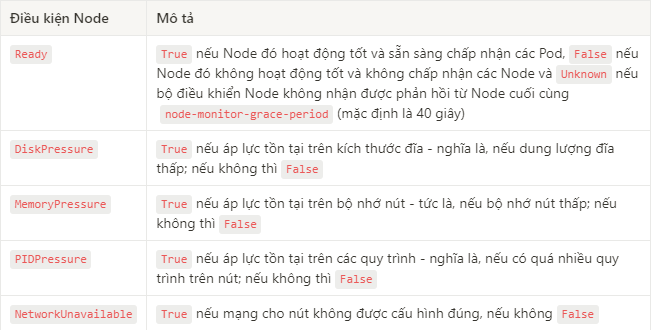
\includegraphics[width=1\linewidth]{Pics/conditions}
			\caption{\label{fig:conditions}Ví dụ về các điều kiện}
			\label{fig:conditions}
		\end{figure}
		\smallskip
		\subitem Trong API Kubernetes, điều kiện của Node được biểu diễn như một phần của \texttt{.status} của tài nguyên Node. Ví dụ: cấu trúc JSON sau đây mô tả một Node hoạt động tốt:
		\smallskip
		\begin{lstlisting}[language=Bash]
			"conditions": [
			{
				"type": "Ready",
				"status": "True",
				"reason": "KubeletReady",
				"message": "kubelet is posting ready status",
				"lastHeartbeatTime": "2019-06-05T18:38:35Z",
				"lastTransitionTime": "2019-06-05T11:41:27Z"
			}
			]
		\end{lstlisting}
		\smallskip
		\subitem Nếu \texttt{status} của Readly vẫn còn tình trạng \texttt{Unknown} hoặc \texttt{False} lâu hơn pod-eviction-timeout (một đối số được chuyển đến kube-controller-manager), thì bộ điều khiển Node sẽ kích hoạt quá trình do khởi tạo API trục xuất cho tất cả các Pod được gán cho Node đó. Thời gian chờ trục xuất mặc định là năm phút. Trong một số trường hợp khi không thể truy cập Node, máy chủ API không thể giao tiếp với kubelet trên Node. Quyết định xóa các Pod không thể được thông báo tới kubelet cho đến khi giao tiếp với máy chủ API được thiết lập lại. Trong thời gian chờ đợi, các Pod được lên lịch xóa có thể tiếp tục chạy trên Node được phân vùng.
		\smallskip
		\subitem Bộ điều khiển nút không buộc xóa các Pod cho đến khi được xác nhận rằng chúng đã ngừng chạy trong cụm. Có thể thấy các Nhóm có thể đang chạy trên một Node không thể truy cập được ở trạng thái \texttt{Terminating} hoặc \texttt{Unknown}. Trong trường hợp Kubernetes không thể suy luận từ cơ sở hạ tầng cơ bản nếu một Node đã rời khỏi cụm vĩnh viễn, quản trị viên cụm có thể cần phải xóa đối tượng Node bằng tay. Việc xóa đối tượng Node khỏi Kubernetes sẽ khiến tất cả các đối tượng Pod đang chạy trên Node bị xóa khỏi máy chủ API và giải phóng tên của chúng.
		\smallskip
		\subitem Khi xảy ra sự cố trên các Node, mặt phẳng điều khiển Kubernetes sẽ tự động tạo các dấu vết phù hợp với các điều kiện ảnh hưởng đến Node. Bộ lập lịch xem xét các yếu tố của Node khi gán một Pod cho một Node. Các Pod cũng có thể có dung sai cho phép chúng chạy trên một Node mặc dù nó có một taint cụ thể.
		\smallskip
		\item \textbf{Năng lực và phân bổ}
		\smallskip
		\subitem Mô tả các tài nguyên có sẵn trên Node: CPU, bộ nhớ và số lượng Pod tối đa có thể được lên lịch trên Node.
		\smallskip
		\subitem Các trường trong khối dung lượng cho biết tổng lượng tài nguyên mà một Node có. Khối có thể phân bổ cho biết lượng tài nguyên trên một Node có sẵn để các Pod thông thường sử dụng.
		\smallskip
		\item \textbf{Thông tin}
		\smallskip
		\subitem Mô tả thông tin chung về Node, chẳng hạn như phiên bản kernel, phiên bản Kubernetes (phiên bản kubelet và kube-proxy), chi tiết container runtime và hệ điều hành mà Node sử dụng. Kubelet thu thập thông tin này từ Node và xuất bản nó vào API Kubernetes.
	\end{itemize}
	
	\subsubsection{Heartbeats}
	
	\hspace{1cm}{Heartbeats, được gửi bởi các Node Kubernetes, giúp cụm xác định tính khả dụng của từng Node và thực hiện hành động khi phát hiện lỗi.\\}
	
	\hspace{0.3cm}{Đối với các Node có hai dạng Heartbeats:}
	\begin{itemize}
		\item cập nhật cho \texttt{.status} của một Node.
		\item Lease: Cho các đối tượng Node mượn trong không gian tên \texttt{kube-node-lease}. Mỗi Node có một đối tượng cho mượn được liên kết.
	\end{itemize}
	\hspace{0.3cm}{So với các bản cập nhật \texttt{.status} của Node, Lease là một tài nguyên nhẹ. Sử dụng Lease cho Heartbeats làm giảm tác động hiệu suất của các bản cập nhật này cho các cụm lớn.\\}
	
	\hspace{0.3cm}{Kubelet chịu trách nhiệm tạo và cập nhật các \texttt{.status} Node cũng như cập nhật các Lease liên quan của chúng.}
	
	\begin{itemize}
		\item Kubelet cập nhật \texttt{.status} của Node khi có thay đổi về trạng thái hoặc nếu không có bản cập nhật nào trong khoảng thời gian đã định cấu hình. Khoảng thời gian mặc định để cập nhật các Node là 5 phút, lâu hơn nhiều so với thời gian chờ mặc định 40 giây cho các Node không thể truy cập.
		\item Kubelet tạo và sau đó cập nhật đối tượng Lease của nó cứ sau 10 giây (khoảng thời gian cập nhật mặc định). Các bản cập nhật Lease xảy ra độc lập với các bản cập nhật cho \texttt{.status} của Node. Nếu cập nhật Lease không thành công, kubelet sẽ thử lại, sử dụng tính năng dự phòng theo cấp số nhân bắt đầu ở 200 mili giây và giới hạn ở 7 giây.
	\end{itemize}
	\subsubsection{Bộ điều khiển Node}
	
	\hspace{1cm}{Bộ điều khiển Node là một thành phần control plane Kubernetes quản lý các khía cạnh khác nhau của các Node.\\}
	
	\hspace{0.3cm}{Bộ điều khiển Node có nhiều vai trò trong vòng đời của Node. Đầu tiên là gán một khối CIDR cho Node khi nó được đăng ký (nếu chức năng gán CIDR được bật).\\}
	
	\hspace{0.3cm}{Thứ hai là giữ cho danh sách các Node nội bộ của bộ điều khiển Node được cập nhật với danh sách các máy có sẵn của nhà cung cấp đám mây. Khi chạy trong môi trường đám mây và bất cứ khi nào một Node không hoạt động tốt, bộ điều khiển Node sẽ hỏi nhà cung cấp đám mây xem VM cho Node đó có còn khả dụng hay không. Nếu không, bộ điều khiển Node sẽ xóa Node đó khỏi danh sách các Node của nó.\\}
	
	\hspace{0.3cm}{	Thứ ba là theo dõi tình trạng của các Node. Bộ điều khiển Node chịu trách nhiệm:}
	
	\begin{itemize}
		\item Trong trường hợp một Node không thể truy cập được, hãy cập nhật điều kiện trong trường \texttt{Ready} của \texttt{.status} Node. Trong trường hợp này, bộ điều khiển Node đặt điều kiện thành \texttt{Unknown}.
		\item Nếu một nút vẫn không thể truy cập: kích hoạt khởi tạo API trục xuất cho tất cả các Pod trên Node không thể truy cập. Theo mặc định, bộ điều khiển Node đợi 5 phút kể từ khi đánh dấu Node là \texttt{Unknown} và gửi yêu cầu trục xuất đầu tiên.
	\end{itemize}
	
	\hspace{0.3cm}{Theo mặc định, bộ điều khiển Node sẽ kiểm tra trạng thái của từng Node sau mỗi 5 giây. Khoảng thời gian này có thể được cấu hình bằng cách sử dụng cờ \texttt{--node-monitor-period} trên thành phần \texttt{kube-controller-manager}.}
	
	\subsection{Giao tiếp giữa các Node và Control Plane}
	
	\hspace{1cm}{Các giao tiếp bao gồm các đường dẫn giao tiếp giữa máy chủ API và cụm Kubernetes. Mục đích là cho phép người dùng tùy chỉnh cài đặt của họ để củng cố cấu hình mạng sao cho cụm có thể chạy trên mạng không đáng tin cậy (hoặc trên các IP công khai hoàn toàn trên nhà cung cấp dịch vụ đám mây).}
	
	\subsubsection{Node tới Control Plane}
	
	\hspace{1cm}{Kubernetes có mẫu API "hub-and-spoke". Tất cả việc sử dụng API từ các Node (hoặc Pod mà chúng chạy) sẽ chấm dứt tại máy chủ API. Không có thành phần Control plane nào khác được thiết kế để hiển thị các dịch vụ từ xa. Máy chủ API được định cấu hình để lắng nghe các kết nối từ xa trên cổng HTTPS an toàn (thường là 443) có bật một hoặc nhiều hình thức xác thực ứng dụng khách . Một hoặc nhiều hình thức ủy quyền phải được bật, đặc biệt nếu các yêu cầu ẩn danh hoặc mã thông báo tài khoản dịch vụ được cho phép.\\}
	
	\hspace{0.3cm}{Các Node phải được cung cấp chứng chỉ gốc công khai cho cụm sao cho chúng có thể kết nối an toàn với máy chủ API cùng với thông tin đăng nhập hợp lệ của ứng dụng khách. Một cách tiếp cận tốt là thông tin xác thực ứng dụng khách được cung cấp cho kubelet ở dạng chứng chỉ ứng dụng khách.\\}
	
	\hspace{0.3cm}{Các Pod muốn kết nối với máy chủ API có thể thực hiện việc này một cách an toàn bằng cách tận dụng tài khoản dịch vụ để Kubernetes sẽ tự động thêm chứng chỉ gốc công khai và mã thông báo hợp lệ vào nhóm khi nó được khởi tạo. Dịch vụ \texttt{kubernetes} (trong không gian tên \texttt{default}) được định cấu hình với một địa chỉ IP ảo được chuyển hướng (thông qua \texttt{kube-proxy}) đến điểm cuối HTTPS trên máy chủ API.\\}
	
	\hspace{0.3cm}{Các thành phần của control plane cũng giao tiếp với máy chủ API qua cổng an toàn.\\}
	
	\hspace{0.3cm}{Do đó, chế độ hoạt động mặc định cho các kết nối từ các Node và Pod chạy trên các Node đến Control plane được bảo mật theo mặc định và có thể chạy trên các mạng công cộng và/hoặc không đáng tin cậy.}
	
	\subsubsection{Control plane tới node}
	
	\hspace{1cm}{Có hai đường dẫn giao tiếp chính từ Control plane (máy chủ API) đến các Node. Đầu tiên là từ máy chủ API đến quy trình kubelet chạy trên mỗi Node trong cụm. Thứ hai là từ máy chủ API đến bất kỳ Node, Pod hoặc Service nào thông qua chức năng proxy của máy chủ API.}
	
	\begin{itemize}
		\item \textbf{API server đến kubelet}
		\smallskip
		\subitem Các kết nối từ máy chủ API đến kubelet được sử dụng cho:
		\begin{itemize}
			\item Tìm nạp nhật ký cho Pod.
			\item Đính kèm (thường thông qua \texttt{kubectl}) vào các Pod đang chạy.
			\item Cung cấp chức năng chuyển tiếp cổng của kubelet.
		\end{itemize}
		\subitem Các kết nối này kết thúc tại điểm cuối HTTPS của kubelet. Theo mặc định, máy chủ API không xác minh chứng chỉ phục vụ của kubelet, điều này làm cho kết nối phải chịu các cuộc tấn công trung gian và không an toàn khi chạy trên các mạng công cộng và/hoặc không đáng tin cậy.
		\smallskip
		\subitem Để xác minh kết nối này, hãy sử dụng cờ \texttt{--kubelet-certificate-authority} để cung cấp cho máy chủ API gói chứng chỉ gốc nhằm sử dụng để xác minh chứng chỉ cung cấp của kubelet.
		\smallskip
		\subitem Nếu không thể, hãy sử dụng đường hầm SSH giữa máy chủ API và kubelet nếu cần để tránh kết nối qua mạng công cộng hoặc không đáng tin cậy.
		\smallskip
		\subitem Cuối cùng, xác thực và/hoặc ủy quyền Kubelet phải được bật để bảo mật API kubelet.
		
		\item \textbf{API server đến các Node, Pod hoặc Service}
		\smallskip
		\subitem Các kết nối từ máy chủ API đến một Node, Pod hoặc Service mặc định là kết nối HTTP đơn giản và do đó không được xác thực cũng như không được mã hóa. Chúng có thể được chạy qua kết nối HTTPS an toàn bằng cách thêm tiền tố \texttt{https:} vào tên Node, Pod hoặc Service trong URL API, nhưng chúng sẽ không xác thực chứng chỉ do điểm cuối HTTPS cung cấp cũng như không cung cấp thông tin đăng nhập của khách hàng. Vì vậy, mặc dù kết nối sẽ được mã hóa nhưng nó sẽ không cung cấp bất kỳ đảm bảo nào về tính toàn vẹn. Các kết nối này hiện không an toàn để chạy qua các mạng công cộng hoặc không đáng tin cậy.
		
		\item \textbf{SSH tunnels}
		\smallskip
		\subitem Kubernetes hỗ trợ các SSH tunnel để bảo vệ các đường dẫn giao tiếp của control plane đến Node. Trong cấu hình này, máy chủ API khởi tạo một SSH tunnel tới từng Node trong cụm (kết nối với máy chủ SSH đang nghe trên cổng 22) và chuyển tất cả lưu lượng dành cho kubelet, Node, Pod hoặc Service qua tunnel. Tunnel này đảm bảo rằng lưu lượng không bị lộ ra bên ngoài mạng mà các Node đang chạy.
		\smallskip
		\subitem \textbf{Lưu ý}: SSH tunnel hiện không được dùng nữa, vì vậy không nên chọn sử dụng chúng trừ khi biết bản thân đang sử dụng với mục đích gì. Dịch vụ Konnectivity là sự thay thế cho kênh liên lạc này.
		
		\item \textbf{Dịch vụ Konnectivity}
		\smallskip
		\subitem Để thay thế cho các SSH tunnel, dịch vụ Konnectivity cung cấp proxy cấp TCP cho mặt phẳng điều khiển để liên lạc theo cụm. Dịch vụ Konnectivity bao gồm hai phần: máy chủ Konnectivity trong mạng control plane và tác nhân Konnectivity trong mạng Node. Tác nhân Konnectivity khởi tạo kết nối đến máy chủ Konnectivity và duy trì kết nối mạng. Sau khi kích hoạt dịch vụ Konnectivity, tất cả lưu lượng truy cập từ control plane đến các Node đều đi qua các kết nối này.
	\end{itemize}

	\subsection{Controllers}
	
	\hspace{1cm}{Trong chế tạo rô-bốt và tự động hóa, vòng lặp điều khiển là một vòng lặp không kết thúc điều chỉnh trạng thái của hệ thống.\\}
	
	\hspace{0.3cm}{Trong Kubernetes, bộ điều khiển là các vòng điều khiển theo dõi trạng thái trong cụm, sau đó thực hiện hoặc yêu cầu thay đổi nếu cần. Mỗi bộ điều khiển cố gắng di chuyển trạng thái cụm hiện tại đến gần trạng thái mong muốn hơn.}
	
	\subsubsection{Kiểu điều khiển}
	
	\hspace{1cm}{Bộ điều khiển theo dõi ít nhất một loại tài nguyên Kubernetes. Các đối tượng này có một trường thông số đại diện cho trạng thái mong muốn. (Các) bộ điều khiển cho tài nguyên đó chịu trách nhiệm làm cho trạng thái hiện tại tiến gần hơn đến trạng thái mong muốn đó.\\}
	
	\hspace{0.3cm}{Bộ điều khiển có thể tự thực hiện hành động; thông thường hơn, trong Kubernetes, bộ điều khiển sẽ gửi tin nhắn đến máy chủ API có tác dụng phụ hữu ích.}
	
	\begin{itemize}
		\item \textbf{Điều khiển thông qua máy chủ API}
		\smallskip
		\subitem Công việc của bộ điều khiển là một ví dụ về bộ điều khiển tích hợp Kubernetes. Bộ điều khiển tích hợp quản lý trạng thái bằng cách tương tác với máy chủ API cụm.
		\smallskip
		\subitem Công việc là một tài nguyên Kubernetes chạy một Pod, hoặc có thể là một số Pod, để thực hiện một tác vụ rồi dừng lại.
		\smallskip
		\subitem (Sau khi được lên lịch , các đối tượng Pod trở thành một phần của trạng thái mong muốn cho một kubelet).
		\smallskip
		\subitem Khi bộ điều khiển Công việc nhìn thấy một tác vụ mới, nó đảm bảo rằng, ở đâu đó trong cụm của bạn, các kubelet trên một nhóm các Node đang chạy đúng số lượng Pod để hoàn thành công việc. Bộ điều khiển công việc không tự chạy bất kỳ các Pod hoặc Container nào. Thay vào đó, bộ điều khiển Công việc yêu cầu máy chủ API tạo hoặc xóa Pod. Các thành phần khác trong control plane hành động dựa trên thông tin mới (có các Pod mới để lên lịch và chạy), và cuối cùng công việc đã hoàn thành.
		\smallskip
		\subitem Sau khi bạn tạo một Công việc mới, trạng thái mong muốn là Công việc đó đã được hoàn thành. Bộ điều khiển Công việc làm cho trạng thái hiện tại của Công việc đó gần với trạng thái mong muốn hơn: tạo các Pod thực hiện làm việc cho Công việc đó, để Công việc gần hoàn thành hơn.
		\smallskip
		\subitem Bộ điều khiển cũng cập nhật các đối tượng cấu hình chúng. Ví dụ: sau khi hoàn thành việc làm cho một Công việc, bộ điều khiển Công việc sẽ cập nhật đối tượng Công việc đó để đánh dấu nó \texttt{Finished}.
		
		\item \textbf{Điều khiển trực tiếp}
		\smallskip
		\subitem Ngược lại với Công việc, một số bộ điều khiển cần thực hiện thay đổi đối với những thứ bên ngoài cụm.
		\smallskip
		\subitem Các bộ điều khiển tương tác với trạng thái bên ngoài sẽ tìm thấy trạng thái mong muốn của chúng từ máy chủ API, sau đó giao tiếp trực tiếp với hệ thống bên ngoài để đưa trạng thái hiện tại đến gần trạng thái mong muốn hơn.
		\smallskip
		\subitem Điểm quan trọng ở đây là bộ điều khiển thực hiện một số thay đổi để mang lại trạng thái mong muốn, sau đó báo cáo trạng thái hiện tại trở lại máy chủ API của cụm. Các vòng điều khiển khác có thể quan sát dữ liệu được báo cáo đó và thực hiện các hành động của riêng chúng.
		\smallskip
		\subitem Với các cụm Kubernetes, control plane hoạt động gián tiếp với các công cụ quản lý địa chỉ IP, dịch vụ lưu trữ, API của nhà cung cấp đám mây và các dịch vụ khác bằng cách mở rộng Kubernetes để triển khai điều đó.
	\end{itemize}
	\subsubsection{Mong muốn so với trạng thái hiện tại}
	
	\hspace{1cm}{Kubernetes có chế độ xem hệ thống dựa trên đám mây và có thể xử lý thay đổi liên tục.\\}
	
	\hspace{0.3cm}{Cụm của bạn có thể thay đổi bất kỳ lúc nào khi công việc diễn ra và các vòng lặp điều khiển sẽ tự động khắc phục lỗi. Điều này có nghĩa là, có khả năng, cụm của bạn không bao giờ đạt đến trạng thái ổn định.\\}
	
	\hspace{0.3cm}{Miễn là các bộ điều khiển cho cụm đang chạy và có thể thực hiện các thay đổi hữu ích, nó không quan trọng nếu trạng thái tổng thể là ổn định hay không.}
	
	\subsubsection{Thiết kế}
	
	\hspace{1cm}{Như một nguyên lý trong thiết kế của nó, Kubernetes sử dụng rất nhiều bộ điều khiển mà mỗi bộ điều khiển quản lý một khía cạnh cụ thể của trạng thái cụm. Thông thường nhất, một vòng lặp điều khiển cụ thể (bộ điều khiển) sử dụng một loại tài nguyên làm trạng thái mong muốn của nó và có một loại tài nguyên khác mà nó quản lý để thực hiện trạng thái mong muốn đó. Ví dụ: bộ điều khiển cho Công việc theo dõi các đối tượng Công việc (để khám phá công việc mới) và các đối tượng Pod (để chạy Công việc, sau đó để xem khi nào công việc kết thúc). Trong trường hợp này, một cái gì đó khác tạo ra Công việc, trong khi bộ điều khiển Công việc tạo ra các Pod.\\}
	
	\hspace{0.3cm}{Thật hữu ích khi có các bộ điều khiển đơn giản thay vì một bộ vòng điều khiển nguyên khối được liên kết với nhau. Bộ điều khiển có thể bị lỗi, vì vậy Kubernetes được thiết kế để cho phép điều đó xảy ra.\\}
	
	\hspace{0.3cm}{\textbf{Ví dụ}: bạn có thể có các Deployment và Công việc; cả hai đều tạo ra các Pod. Bộ điều khiển công việc không xóa các Pod mà Deployment của bạn đã tạo, vì có thông tin (nhãn) bộ điều khiển có thể sử dụng để phân biệt các Pod đó.}
	
	\subsubsection{Các cách chạy bộ điều khiển}
	
	\hspace{1cm}{Kubernetes đi kèm với một bộ điều khiển tích hợp chạy bên trong kube-controller-manager. Các bộ điều khiển tích hợp này cung cấp các hành vi cốt lõi quan trọng.\\}
	
	\hspace{0.3cm}{Bộ điều khiển Deployment và Bộ điều khiển công việc là những ví dụ về bộ điều khiển là một phần của chính Kubernetes (bộ điều khiển "tích hợp"). Kubernetes cho phép bạn chạy một control plane có khả năng đối phó để nếu bất kỳ bộ điều khiển tích hợp nào bị lỗi, một phần khác của control plane sẽ đảm nhận công việc.\\}
	
	\hspace{0.3cm}{Bạn có thể tìm các bộ điều khiển chạy bên ngoài control plane để mở rộng Kubernetes. Hoặc, nếu muốn, bạn có thể tự viết một bộ điều khiển mới. Bạn có thể chạy bộ điều khiển của riêng mình dưới dạng một bộ Pod hoặc bên ngoài Kubernetes. Những gì phù hợp nhất sẽ phụ thuộc vào chức năng của bộ điều khiển cụ thể đó.}
	
	\section{Cơ cấu tổ chức}
	\section{Chức năng của từng bộ phận}
	\section{Cơ cấu nguồn nhân lực}
	\section{Các lĩnh vực hoạt động kinh doanh và sản xuất}
	\section{Chiến lược, định hướng phát triển trong thời gian tới}
	\hspace{1.0cm} {Microservices không còn là một điều mới lạ. Chúng ta đang thấy vi mô quy mô lớn triển khai dịch vụ với hàng ngàn dịch vụ. Nhưng cho dù có một hoặc hai dịch vụ hay hàng nghìn dịch vụ, bảo mật vẫn là ưu tiên hàng đầu.}
	\subsection{Cách bảo mật hoạt động trong ứng dụng monolithic}
	\hspace{1.0cm} {Một ứng dụng monolithic có một vài điểm kết nối. Một điểm vào cho một ứng dụng là một cánh cửa trong một tòa nhà. Giống như một cánh cửa cho phép bạn vào một tòa nhà (có thể sau khi kiểm tra an ninh), một điểm vào ứng dụng cho phép các yêu cầu của bạn vào. \\}
	
	\hspace{0.3cm}{Hãy nghĩ về một ứng dụng web chạy trên cổng HTTP mặc định 80 trên một máy chủ mang địa chỉ IP 192.168.0.1. Cổng 80 trên máy chủ 192.168.0.1 là một điểm vào ứng dụng web đó. Nếu cùng một ứng dụng web chấp nhận các yêu cầu HTTPS trên cùng một máy chủ trên cổng 443, thì sẽ có một điểm vào khác. Khi ứng dụng có nhiều điểm vào hơn, người quản trị có nhiều nơi hơn để lo lắng về việc bảo mật. Càng nhiều điểm vào một ứng dụng, bề mặt tấn công càng rộng.}
	\begin{figure}[h]
		\centering
		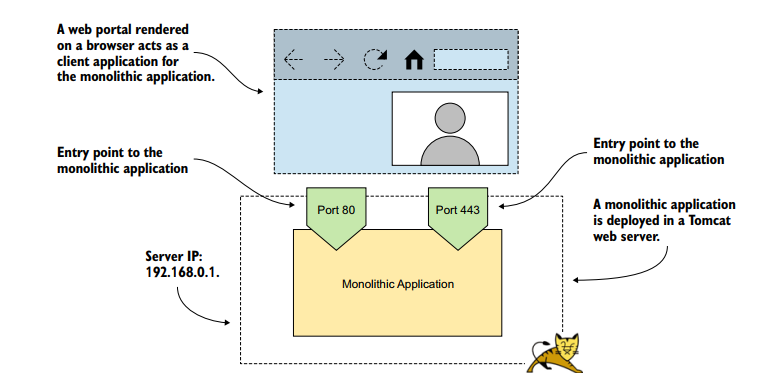
\includegraphics[width=0.7\linewidth]{Pics/monolithic-1}
		\caption{\label{fig:nodes} Ứng dụng monolithich cơ bản.}
		\label{fig:nodes}
	\end{figure}
	\hspace{0.3cm}{Trong hầu hết các ứng dụng nguyên khối, bảo mật được thực thi tập trung và các thành phần riêng lẻ không cần phải lo lắng về việc thực hiện các kiểm tra bổ sung trừ khi có yêu cầu khẩn cấp để
	làm như vậy. Do đó, mô hình bảo mật của ứng dụng nguyên khối đơn giản hơn nhiều so với mô hình bảo mật của ứng dụng được xây dựng trên kiến trúc microservice.}

	\subsection{Nguyên tắc cơ bản trong bảo mật bảo mật microservice}
	\subsubsection{Tính xác thực}
	\hspace{1.0cm}{Xác thực là quá trình xác định bên yêu cầu để bảo vệ hệ thống của bạn chống giả mạo. Bên yêu cầu có thể là một hệ thống (một microservice) hoặc một hệ thống yêu cầu quyền truy cập thay mặt cho người dùng là con người hoặc một hệ thống khác. Tuy nhiên, rất khó có khả năng người dùng là con người sẽ truy cập trực tiếp vào một microservice. Trước khi tạo một thiết kế bảo mật cho một hệ thống nhất định, bạn cần xác định đối tượng. Phương pháp xác thực bạn chọn dựa trên đối tượng.\\}
	
	\begin{figure}[h]
		\centering
		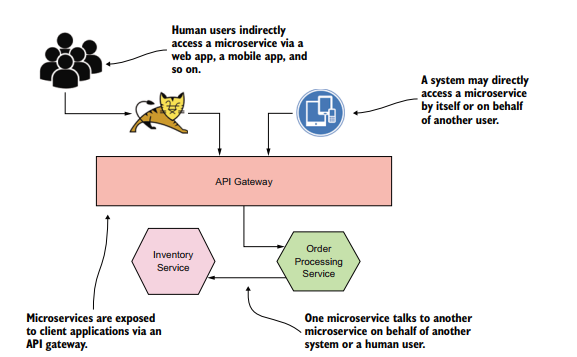
\includegraphics[width=0.7\linewidth]{Pics/authentication}
		\caption{\label{fig:nodes} Các đối tượng xác thực.}
		\label{fig:nodes}
	\end{figure}

	\hspace{0.3cm}{Để xác thực người dùng với một hệ thống (ví dụ: ứng dụng web), ứng dụng có thể yêu cầu tên người dùng và mật khẩu với một yếu tố khác cho xác thực đa yếu tố (MFA). MFA có bắt buộc hay không chủ yếu là do quyết định kinh doanh, dựa trên mức độ quan trọng của tài sản kinh doanh của bạn hoặc mức độ nhạy cảm của dữ liệu bạn muốn chia sẻ với người dùng.}

	\subsubsection{Tính toàn vẹn}
	\hspace{1.0cm}{Khi bạn truyền dữ liệu từ ứng dụng khách của mình sang một vi dịch vụ hoặc từ một vi dịch vụ này sang một vi dịch vụ khác—tùy thuộc vào độ mạnh của kênh liên lạc mà bạn chọn—kẻ xâm nhập có thể chặn liên lạc và thay đổi dữ liệu để có lợi cho chúng. Ví dụ: nếu kênh mang dữ liệu tương ứng với một đơn đặt hàng, thì kẻ xâm nhập có thể thay đổi địa chỉ giao hàng thành địa chỉ của chính họ. Các hệ thống được bảo vệ cho tính toàn vẹn không bỏ qua khả năng này; họ giới thiệu các biện pháp để nếu một tin nhắn bị thay đổi, người nhận có thể phát hiện và loại bỏ yêu cầu.\\}
	
	\hspace{0.3cm}{Cách phổ biến nhất để bảo vệ tính toàn vẹn của một thông điệp là ký tên vào nó.Mọi dữ liệu truyền qua kênh liên lạc được bảo vệ bằng Bảo mật tầng truyền tải (TLS) đều được bảo vệ toàn vẹn. Nếu chúng ta sử dụng HTTPS để liên lạc giữa các vi dịch vụ (trên thực tế, giao tiếp đó là HTTP qua TLS), thư sẽ được bảo vệ toàn vẹn trong khi truyền.\\}
	
	\hspace{0.3cm}{Cùng với dữ liệu đang truyền, dữ liệu ở trạng thái nghỉ phải được bảo vệ toàn vẹn. Trong tất cả dữ liệu kinh doanh, các dấu vết kiểm tra quan trọng nhất để kiểm tra tính toàn vẹn. Kẻ xâm nhập có quyền truy cập vào hệ thống sẽ hạnh phúc nếu họ có thể sửa đổi các dấu vết kiểm tra để xóa sạch mọi bằng chứng. Trong quá trình triển khai vi dịch vụ dựa trên container, nhật ký kiểm tra không được lưu giữ ở mỗi nút chạy vi dịch vụ; chúng được xuất bản trong một số loại hệ thống theo dõi phân tán như Jaeger hoặc Zipkin. Chúng ta cần đảm bảo rằng dữ liệu được duy trì trong các hệ thống đó được bảo vệ toàn vẹn.}
	
	\subsubsection{Tính chống chối bỏ}
	\hspace{1.0cm}{Chống chối bỏ là một khía cạnh quan trọng của bảo mật thông tin ngăn cản bạn từ chối bất cứ điều gì bạn đã thực hiện hoặc cam kết. Hãy xem xét một ví dụ thực tế. Khi bạn thuê một căn hộ, bạn đồng ý với các điều khoản và điều kiện với công ty cho thuê.\\}
	
	\hspace{0.3cm}{Nếu bạn rời khỏi căn hộ trước khi kết thúc hợp đồng thuê, bạn có nghĩa vụ trả tiền thuê cho thời gian còn lại hoặc tìm người thuê khác để thuê lại căn hộ. Tất cả các điều khoản đều có trong hợp đồng cho thuê mà bạn chấp nhận bằng cách ký tên vào đó. Sau khi bạn ký tên, bạn không thể tranh chấp các điều khoản và điều kiện mà bạn đã đồng ý. Đó là điều không thể phủ nhận trong thế giới thực. Nó tạo ra một nghĩa vụ pháp lý. Ngay cả trong thế giới kỹ thuật số, một chữ ký giúp bạn đạt được sự không từ chối; trong trường hợp này, bạn sử dụng chữ ký điện tử.\\}
	
	\hspace{0.3cm}{Bạn cũng cần đảm bảo rằng bạn ghi lại các giao dịch cùng với dấu thời gian và chữ ký—đồng thời duy trì các bản ghi đó trong một khoảng thời gian đáng kể. Trong trường hợp người khởi xướng tranh chấp giao dịch sau này, bạn sẽ có giao dịch đó trong hồ sơ của mình.}
	
	\subsubsection{Tính sẵn sàng}
	\hspace{1.0cm}{Toàn bộ quan điểm của việc xây dựng bất kỳ loại hệ thống nào là cung cấp cho người dùng. Cứ mỗi phút (hoặc thậm chí là giây) hệ thống ngừng hoạt động, doanh nghiệp của bạn sẽ mất tiền. Amazon đã ngừng hoạt động trong 20 phút vào tháng 3 năm 2016 và tổn thất doanh thu ước tính là 3,75 triệu USD. Vào tháng 1 năm 2017, hơn 170 chuyến bay của Delta Airlines đã bị hủy do hệ thống ngừng hoạt động, dẫn đến thiệt hại ước tính 8,5 triệu USD.\\}
	
	\hspace{0.3cm}{Không giống như trong các ứng dụng nguyên khối, trong triển khai vi dịch vụ, toàn bộ hệ thống sẽ không ngừng hoạt động nếu phát hiện thấy lỗi trong một thành phần hoặc vi dịch vụ. Chỉ microservice đó sẽ ngừng hoạt động; phần còn lại sẽ có thể hoạt động. Trong tất cả các yếu tố có thể làm hệ thống ngừng hoạt động, bảo mật có vai trò then chốt trong việc giúp hệ thống luôn sẵn sàng cho các bên liên quan hợp pháp của nó. Trong triển khai microservices, với nhiều điểm vào (có thể tiếp xúc với internet), kẻ tấn công có thể thực hiện tấn công từ chối dịch vụ (DoS) hoặc tấn công từ chối dịch vụ phân tán (DDoS) và đánh sập hệ thống.\\}
	
	\hspace{0.3cm}{Phòng thủ chống lại các cuộc tấn công như vậy có thể được xây dựng trên các cấp độ khác nhau. Ở cấp độ ứng dụng, điều tốt nhất bạn có thể làm là từ chối một tin nhắn (hoặc một yêu cầu) ngay khi bạn thấy rằng nó không hợp pháp. Có kiến trúc bảo mật theo lớp giúp bạn thiết kế từng lớp để xử lý các loại tấn công khác nhau và từ chối kẻ tấn công ở lớp ngoài cùng.}
	
	\pagebreak
	
	\section{Kết luận chương 1}

	\hspace{0.8cm}{Qua chương một, chúng ta đã tìm hiểu về kubernetes là gì, kiến trúc và cách thức hoạt động của kubernetes. Và tổng quan về microservice, các nguyên tắc để bảo vệ microservice. Nhưng khi mà chúng ta triển khai hệ thống microservice trên kubernetes, chúng ta làm thế nào để có thể bảo mật được các microservice. Nếu như một hệ thống lớn, có hàng trăm đến hàng ngàn microservice, thì liệu chúng ta có thể chỉ cần triển khai bảo mật trên hệ thống mà không cần phải sửa lại tất cả microservice đó không. Điều này là có thể đối với Service Mesh, một trong những công nghệ giúp chúng ta triển khai trên mặt hệ thống giúp bảo mật các ứng dụng microservice. Vậy, service mesh là gì, cách hoạt động của nó như nào, chúng ta sẽ đến với chương 2. Ở chương 2, chúng ta sẽ nói tổng quan về service mesh và công cụ giúp chúng ta triển khai service mesh trên kubernetes là HashiCorp Consul.}
	
	\chapter{Giới thiệu về HashiCorp Consul}
	
	\section{Tổng quát về Service Mesh}
	
	\hspace{1.0cm}{Để bắt đầu hành trình khám phá service mesh, có ba điều mà chúng ta cần phải biết: Service Mesh là gì, cách thức nó hoạt động như nào và tại sao chúng ta lại sử dụng nó.\\}
	
	\hspace{0.3cm}{Có lẽ, để định nghĩa ngắn gọn service mesh, thì chúng ta có thể hiểu như sau:\\}
	
	\hspace{0.8cm}{Service mesh là lớp kiến trúc hạ tầng mà cho phép bạn kiểm soát giao tiếp mạng của hệ thống của bạn từ một control plan duy nhất.\\}
	
	\hspace{0.3cm}{Để hiểu hơn về định nghĩa trên, chúng ta cần chia thành các phần sau: \\}
	
	\hspace{0.3cm}{Thông qua lớp kiến trúc hạ tầng, service mesh không phải là một phần của service, nó được triển khai và vận hành theo một cách độc lập. Vì nó không thể xác định được cụ thể được logic hoạt động của dịch vụ cụ thể, nhưng nó ảnh hưởng đến mọi dịch vụ, nên nó được coi là cơ sở hạ tầng hoặc phần mềm trung gian.\\}
	
	\hspace{0.3cm}{Dưới đây là hình ảnh của một phần mềm thông thường. Dịch vụ và ứng dụng chạy trên các cơ sở hạ tầng. Service mesh nằmg ở lớp cơ sở hạ tầng đầu tiên với các yêu cầu về lưu trữ, metrics và cơ sở hạ tầng cao cấp khác. Bến dưới đó là Kubernetes, máy ảo hoặc bất kì kiến trúc máy tính nào mà có thể chạy. Bên dưới cùng là phần cứng (bare metal)\\}
	
	\begin{figure}[h]
		\centering
		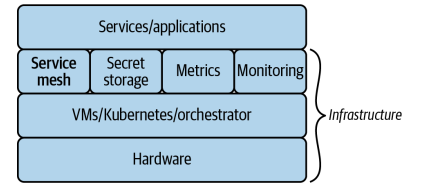
\includegraphics[width=0.7\linewidth]{Pics/software_stack}
		\caption{\label{fig:software_stack} Một khối ứng dụng cụ thể}
		\label{fig:software_stack}
	\end{figure}
	
	\subsection{Phương thức hoạt động của service mesh}
	\hspace{1.0cm}{Service mesh được tạo thành từ các proxy sidecar và control plan.}
	\subsubsection{Proxy Sidecar}
	\hspace{1.0cm}{Proxy là một ứng dụng mà lưu lượng truy cập được định tuyến trên đường đến đích của nó. Các proxy phổ biến mà bạn có thể đã nghe nói đến là NGINX, HAProxy và Envoy. Trong hầu hết các service mesh, tất cả lưu lượng dịch vụ (vào và ra) được định tuyến thông qua một proxy cục bộ dành riêng cho từng phiên bản dịch vụ\\}
	
	\hspace{0.3cm}{Hình bên dưới thể hiện service mesh sẽ như thế nào với 2 đối tượng: frontend và backend. Khí frontend gọi đến backend, proxy cục bộ của frontend sẽ bắt tất cả các yêu cầu được đi ra ngoài. Proxy của frontend sẽ chuyển các yêu cầu đến dịch vụ backend. Khi mà yêu cầu được đưa tới dịch vụ backend, tiếp tục, nó được proxy cục bộ của backend nắm bắt và kiểm tra. Nếu yêu cầu được cho phép, proxy của backend sẽ chuyển tiếp yêu cầu đó đên dịch vụ backend thực tế.\\}
	\begin{figure}[h]
		\centering
		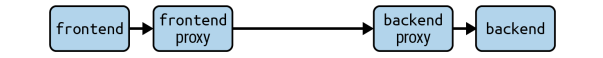
\includegraphics[width=0.7\linewidth]{Pics/proxy}
		\caption{\label{fig:proxy} Hai ứng dụng giao tiếp với nhau thông qua service mesh}
		\label{fig:proxy}
	\end{figure}
	
	\hspace{0.3cm}{Mỗi phiên bản của một dịch vụ phải được triển khai với proxy cục bộ của chính nó. Mẫu triển khai ứng dụng trợ giúp - trong trường hợp này là proxy - cùng với dịch vụ chính được gọi là mẫu sidecar và do đó, proxy cục bộ được gọi là proxy sidecar.\\}
	
	\hspace{0.3cm}{Proxy Sidecar là một thành phần quan trọng của service mesh vì chúng cho phép kiểm soát lưu lượng dịch vụ mà không cần sửa đổi hoặc triển khai lại các dịch vụ cơ bản. Vì proxy sidecar chạy dưới dạng các quy trình riêng biệt với dịch vụ nên chúng có thể được cấu hình lại mà không ảnh hưởng đến dịch vụ. Ví dụ: proxy sidecar của dịch vụ backend có thể được cấu hình lại để từ chối lưu lượng truy cập từ dịch vụ backend mà không cần thay đổi mã hoặc triển khai lại chính dịch vụ backend.}
	
	\subsubsection{Control Plane}
	\hspace{1.0cm}{Công việc của control plane là quản lý và định cấu hình các proxy sidecar. Như bạn có thể thấy hình bên dưới, control plane là một dịch vụ riêng biệt phải được triển khai riêng; nó không được triển khai như một sidecar. control plane là nơi chứa hầu hết logic phức tạp của service mesh: nó phải theo dõi các dịch vụ bắt đầu và dừng, ký và phân phối chứng chỉ, cấu hình lại proxy, v.v. Bản thân các proxy sidecar tương đối đơn giản: chúng nhận cấu hình từ control plane nêu chi tiết những hành động nào sẽ thực hiện trên lưu lượng truy cập và họ thực hiện những hành động đó.}
	\begin{figure}[h]
		\centering
		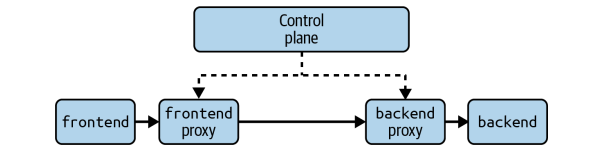
\includegraphics[width=0.7\linewidth]{Pics/control-plane}
		\caption{\label{fig:control-plane} Control plane quản lý các sidecar proxy.}
		\label{fig:control-plane}
	\end{figure}

	\subsection{Các tính năng của service mesh}
	\hspace{1.0cm}{Service mesh cung cấp các tính năng trong bốn lĩnh vực: bảo mật, khả năng quan sát, độ tin cậy và kiểm soát lưu lượng. Đề xuất giá trị cơ bản của service mesh là khả năng cung cấp các tính năng này trên mọi dịch vụ và khối lượng công việc mà không cần sửa đổi mã dịch vụ.}
	\subsubsection{Bảo mật}
	\hspace{1.0cm}{Một trong những lý do chính khiến các công ty triển khai service mesh là để bảo mật mạng của họ. Thông thường, điều này có nghĩa là mã hóa lưu lượng giữa tất cả các khối lượng công việc và triển khai xác thực cũng như ủy quyền.\\}
	
	\hspace{0.3cm}{Giải quyết vấn đề này có thể rất khó khăn trong kiến trúc microservices mà không có service mesh. Yêu cầu mã hóa mọi yêu cầu có nghĩa là cung cấp chứng chỉ Bảo mật tầng vận chuyển (TLS) cho mọi dịch vụ theo cách an toàn và quản lý cơ sở hạ tầng ký chứng chỉ của riêng bạn. Xác thực và ủy quyền mọi yêu cầu có nghĩa là cập nhật và duy trì mã xác thực trong mọi dịch vụ.\\}
	
	\hspace{0.3cm}{Service mesh giúp công việc này dễ dàng hơn nhiều vì nó có thể cấp chứng chỉ và định cấu hình proxy sidecar để mã hóa lưu lượng và thực hiện ủy quyền - tất cả mà không có bất kỳ thay đổi nào đối với các dịch vụ cơ bản\\}
	
	\begin{figure}[h]
		\centering
		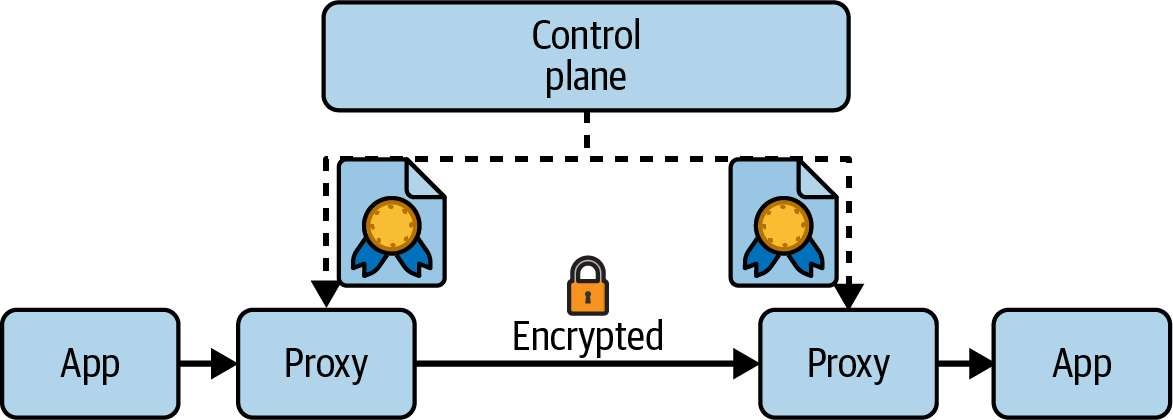
\includegraphics[width=0.7\linewidth]{Pics/service-mesh_encrypted}
		\caption{\label{fig:service-meshencrypted} Service mesh phát hành chứng chỉ và mã hóa đường truyền. }
		\label{fig:service-meshencrypted}
	\end{figure}

	\subsubsection{Khả năng quan sát}
	\hspace{1cm}{Khả năng quan sát là khả năng hiểu điều gì đang xảy ra với các dịch vụ của bạn khi chúng đang chạy. Dữ liệu về khả năng quan sát là cần thiết để hiểu kiến trúc vi dịch vụ và chẩn đoán lỗi, nhưng việc định cấu hình tất cả các dịch vụ của bạn để phát ra các chỉ số và dữ liệu khác theo cách thống nhất có thể là một thách thức.\\}
	
	\hspace{0.3cm}{Nắm bắt dữ liệu quan sát được là công việc hoàn hảo cho service mesh vì tất cả các yêu cầu đều chảy qua proxy của nó. Service mesh có thể định cấu hình proxy của nó để phát ra số liệu trên tất cả các dịch vụ của bạn ở định dạng nhất quán mà không cần sửa đổi hoặc triển khai lại các dịch vụ cơ bản.}
	
	\subsubsection{Độ tin cậy}
	\hspace{1cm}{Trong các hệ thống phân tán, thường có lỗi xảy ra. Xây dựng các hệ thống phân tán đáng tin cậy có nghĩa là giảm thiểu sự cố nếu có thể và xử lý sự cố một cách khéo léo khi nó chắc chắn xảy ra.\\}
	
	\hspace{0.3cm}{Giảm thất bại có thể có nghĩa là thực hiện kiểm tra tình trạng để lưu lượng truy cập chỉ được gửi đến các dịch vụ khỏe mạnh. Xử lý lỗi có thể có nghĩa là thử lại các yêu cầu không thành công hoặc triển khai thời gian chờ, vì vậy một dịch vụ không chờ phản hồi mãi mãi.\\}
	
	\hspace{0.3cm}{Việc triển khai các kỹ thuật này trong mã tốn nhiều thời gian, dễ xảy ra lỗi và khó thực hiện một cách nhất quán trên tất cả các dịch vụ của bạn. Với service mesh, proxy có thể thực hiện các kỹ thuật này cho bất kỳ dịch vụ nào của bạn - tất cả những gì bạn cần làm là tương tác với control plane. Bạn cũng có thể điều chỉnh cài đặt theo thời gian thực khi tải dịch vụ thay đổi.\\}
	
	\begin{figure}[h]
		\centering
		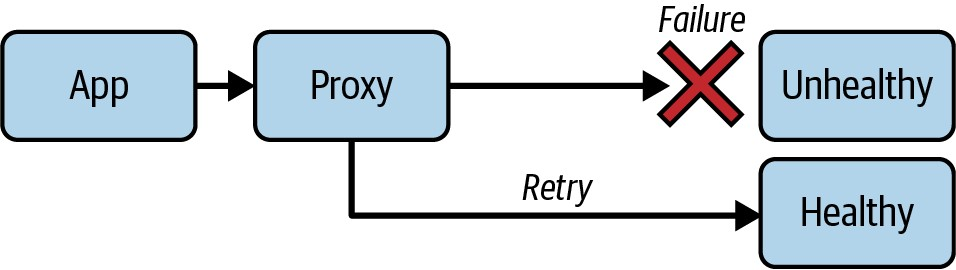
\includegraphics[width=0.7\linewidth]{Pics/reliability}
		\caption{\label{fig:reliability} Service mesh có thể được cấu hình để thử lại các yêu cầu không thành công cho các trường hợp khác.}
		\label{fig:reliability}
	\end{figure}
	
	\subsubsection{Kiểm soát lưu lượng}
	\hspace{1cm}{Kiểm soát lưu lượng là về việc kiểm soát nơi lưu lượng giữa các dịch vụ được định tuyến. Kiểm soát lưu lượng giải quyết nhiều vấn đề:}
	
	\begin{itemize}
		\item Triển khai các chiến lược triển khai, chẳng hạn như triển khai canary, trong đó một lượng nhỏ  lưu lượng truy cập "canary" được chuyển đến phiên bản mới của dịch vụ để xem liệu dịch vụ đó có hoạt động hay không trước khi triển khai đầy đủ phiên bản mới.
		\smallskip
		\item Di chuyển từ nguyên khối sang vi dịch vụ, trong đó các dịch vụ được tách ra khỏi nguyên khối và lưu lượng truy cập trước đây được định tuyến đến nguyên khối được định tuyến lại một cách liền mạch đến các microservice mới.
		\smallskip
		\item Chuyển đổi dự phòng đa cụm, trong đó lưu lượng được định tuyến đến các dịch vụ trong cụm lành mạnh khác nếu cụm cục bộ ngừng hoạt động.
	\end{itemize}

	\subsubsection{Tính năng kết hợp}
	\hspace{1cm}{Bây giờ các loại tính năng mà service mesh cung cấp là về bảo mật, khả năng quan sát, độ tin cậy và kiểm soát lưu lượng. Một mình, các tính năng này rất hữu ích, nhưng chúng thậm chí còn mạnh mẽ hơn khi kết hợp.\\}
	
	\hspace{0.3cm}{Ví dụ: dữ liệu về khả năng quan sát được cung cấp bởi service mesh có thể được kết hợp với các tính năng kiểm soát lưu lượng và độ tin cậy. Nếu lưới phát hiện ra rằng một phiên bản dịch vụ đang trả về lỗi, nó có thể chuyển hướng lưu lượng truy cập đến các phiên bản khỏe mạnh hoặc một cụm hoàn toàn khác. Hoặc các tính năng bảo mật dạng lưới có thể được kết hợp với các tính năng có thể quan sát để phát hiện khi một dịch vụ đang cố thực hiện các yêu cầu mà dịch vụ đó không được phép thực hiện - có khả năng chỉ ra một vi phạm bảo mật. Khi bạn tự triển khai Consul, bạn sẽ thấy nhiều trường hợp sử dụng mà bạn có thể kết hợp các tính năng service mesh.\\}
	
	\hspace{0.3cm}{Nếu tổ chức của bạn cần những tính năng này, thì bạn phải quyết định xem nó có xứng đáng với độ phức tạp bổ sung của service mesh hay không hay liệu bạn có nên triển khai chúng trong mã dịch vụ hay không. Chìa khóa để trả lời câu hỏi đó là kiểm tra quy mô của bạn.\\}
	
	\subsection{Khi nào nên sử dụng service mesh}
	\hspace{1cm}{Không còn nghi ngờ gì nữa, việc triển khai service mesh sẽ làm tăng thêm độ phức tạp. Bây giờ bạn có proxy sidecar và control plane service mesh để quản lý. Ngoài ra, bạn sẽ cần nhiều tài nguyên điện toán hơn (CPU và bộ nhớ) để chạy proxy và control plane, và giờ đây, tất cả lưu lượng truy cập sẽ mất thêm một bước nhảy qua các proxy sidecar cục bộ, điều này làm tăng thêm độ trễ. Việc triển khai các tính năng service mesh trong mã sẽ tiết kiệm tài nguyên và giảm độ phức tạp của cơ sở hạ tầng (mặc dù nó sẽ làm tăng độ phức tạp của mã). Để một service mesh xứng đáng, nó phải cung cấp nhiều giá trị cho tổ chức của bạn.\\}
	
	\hspace{0.3cm}{Một công thức đơn giản để biết khi nào nên sử dụng service mesh là khi bạn (a) cần giải quyết các vấn đề về mạng trong các lĩnh vực đã nêu trước đó (bảo mật, khả năng quan sát, độ tin cậy và kiểm soát lưu lượng) và (b) tổ chức của bạn ở quy mô lớn, hoặc sẽ sớm đạt đến quy mô mà việc giải quyết những vấn đề đó trong mã dịch vụ là quá tốn kém.\\}
	
	\hspace{0.3cm}{Ví dụ: giả sử tổ chức của bạn đang chuyển sang kiến trúc bảo mật không tin cậy, trong đó tất cả lưu lượng truy cập nội bộ được mã hóa, xác thực và ủy quyền. Nếu chỉ chạy hai vi dịch vụ, bạn có thể dễ dàng mã hóa lại các dịch vụ đó. Tuy nhiên, nếu bạn đang chạy 400 vi dịch vụ, thì bạn sẽ không thể mã hóa lại tất cả các dịch vụ đó trong một khoảng thời gian hợp lý. Trong trường hợp này, một service mesh có rất nhiều ý nghĩa.\\}
	
	\hspace{0.3cm}{Ngoài ra, ở một quy mô nhất định, sẽ có các dịch vụ và khối lượng công việc mà bạn muốn kiểm soát mà bạn thực sự không có khả năng chỉnh sửa mã của chúng. Ví dụ: có thể bạn đang triển khai một phần mềm nguồn mở được đóng gói hoặc có thể bạn đang sử dụng cơ sở dữ liệu do đám mây quản lý. Lý tưởng nhất là bạn sẽ có cùng quyền kiểm soát đối với những khối lượng công việc mà bạn thực hiện đối với các dịch vụ khác của mình.\\}
	
	\hspace{0.3cm}{Cuối cùng, quy mô chính xác mà việc sử dụng service mesh hợp lý sẽ phụ thuộc vào tổ chức cụ thể của bạn và các vấn đề bạn đang cố gắng giải quyết. Tôi hy vọng rằng cuốn sách này sẽ giúp bạn hiểu các vấn đề mà service mesh giải quyết và giúp bạn đánh giá xem nó có hợp lý trong tình huống của bạn hay không.}
	
	\section{Giới thiệu về Consul}
	\hspace{1cm}{“Hôm nay chúng tôi công bố Consul, một giải pháp để khám phá và cấu hình dịch vụ. Consul được phân phối hoàn toàn, có tính sẵn sàng cao và mở rộng quy mô thành hàng nghìn nút và dịch vụ trên nhiều trung tâm dữ liệu.”}
	
	\hspace{2cm}{- Armon Dadgar (đồng sáng lập HashiCorp), tháng 4 năm 2014\\}
	
	\hspace{0.3cm}{Khi Consul lần đầu tiên xuất hiện vào năm 2014. Điện toán đám mây và kiến trúc hướng dịch vụ (tiền thân của vi dịch vụ) đang trở thành xu hướng chủ đạo và mọi công ty bắt đầu vật lộn với vấn đề làm thế nào để định tuyến đến các dịch vụ và xử lý lỗi trong một hệ thống phân phối.\\}
	
	\hspace{0.3cm}{Consul là một công nghệ mang tính cách mạng vì nó kết hợp khám phá dịch vụ dựa trên DNS với một hệ thống phát hiện lỗi mạnh mẽ. Một dịch vụ sẽ đăng ký vào Consul và các dịch vụ khác có thể sử dụng mục nhập DNS của Consul để định tuyến đến nó. Ví dụ: dịch vụ giao diện người dùng sẽ có sẵn tại frontend.service.consul. Consul cũng phát hiện lỗi bằng cách sử dụng một thuật toán buôn chuyện có tên là Serf (được đề cập ở phần sau của chương này) và kiểm tra sức khỏe. Nếu một nút hoặc dịch vụ gặp sự cố, Consul sẽ nhanh chóng nhận thấy và xóa nó khỏi DNS.\\}
	
	\hspace{0.3cm}{Consul là mã nguồn mở, miễn phí sử dụng và giải quyết vấn đề mà hàng nghìn công ty gặp phải một cách tinh tế. Ngành công nghiệp nhanh chóng áp dụng nó.\\}
	
	\hspace{0.3cm}{Theo thời gian, kiến trúc hướng dịch vụ ngày càng lớn hơn và trở thành kiến trúc microservice với các dịch vụ ngày càng nhỏ hơn. Điều này dẫn đến sự gia tăng của Docker và bộ điều phối container như Kubernetes. Phong trào microservices và Kubernetes đã thay đổi ngành theo hai cách quan trọng:\\}
	
	\hspace{0.3cm}{Đầu tiên, khám phá dịch vụ DNS không còn đủ nữa. Các nhà phát triển cần nhiều tính năng làm việc trên mạng hơn về bảo mật, khả năng quan sát, độ tin cậy và kiểm soát lưu lượng để giúp chạy tất cả các dịch vụ này. Việc triển khai các tính năng này trong mã dịch vụ cũng trở nên khó khăn hơn vì số lượng dịch vụ không ngừng tăng lên.\\}
	
	\hspace{0.3cm}{Thứ hai, Kubernetes giúp việc chạy sidecar proxy trở nên dễ dàng hơn nhiều nhờ vào mô hình nhóm, trong đó nhiều vùng chứa có thể chạy cùng nhau trong một mạng riêng (Trước đây, có thể chạy hai quy trình cùng nhau; tuy nhiên, điều đó khó khăn hơn vì bạn cần phải sắp xếp việc triển khai và cấu hình của chúng theo cách thủ công. Ngoài ra, các quy trình khác trên cùng một máy có thể truy cập cùng một mạng và hệ thống tệp.)\\}
	
	\hspace{0.3cm}{Những thay đổi này đã kích hoạt công nghệ service mesh như chúng ta biết ngày nay.\\}
	
	\hspace{0.3cm}{Nhóm Consul tại HashiCorp đã đi theo những xu hướng này và vào năm 2018, họ đã phát hành một tính năng service mesh có tên là Consul Connect. Consul Connect tập trung vào liên lạc an toàn giữa các dịch vụ và hỗ trợ thêm cho các proxy sidecar để mã hóa lưu lượng giữa các dịch vụ. Kể từ đó, Consul đã phát triển thành một mạng service mesh đầy đủ chức năng với các tính năng không chỉ liên quan đến liên lạc an toàn mà còn cả khả năng quan sát, độ tin cậy và kiểm soát lưu lượng.\\}
	
	\hspace{0.3cm}{Bỏ qua lịch sử đó, bạn đã sẵn sàng tìm hiểu về cách thức hoạt động của Consul và điều gì làm cho nó trở nên độc đáo với tư cách là một mạng service mesh. Các phần sau đây đề cập đến kiến trúc của Consul và các giao thức mà nó sử dụng để duy trì độ tin cậy và khả năng mở rộng.\\}
	
	\subsection{Kiến trúc}
	\hspace{1cm}{Một bản cài đặt Consul được tạo thành từ ba bộ thành phần: máy chủ Consul, ứng dụng client Consul và proxy sidecar. Các proxy Sidecar nói chuyện với các client Consul local của họ và các client Consul nói chuyện với các máy chủ Consul. Thường có ba hoặc năm Node máy chủ Consul  và có thể có tới hàng nghìn Node khối lượng công việc.\\}
	
	\begin{figure}[h]
		\centering
		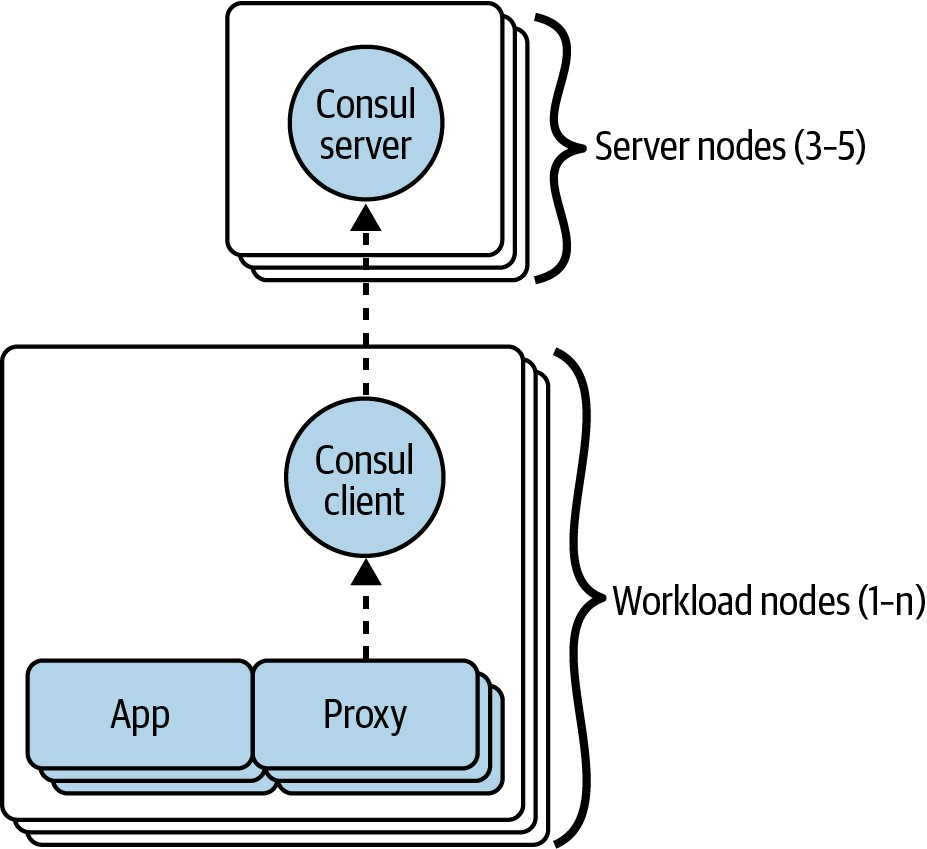
\includegraphics[width=0.7\linewidth]{Pics/architecture}
		\caption{\label{fig:architecture} Bản cài đặt Consul bao gồm máy chủ Consul, máy client Consul và proxy sidecar.}
		\label{fig:architecture}
	\end{figure}
	
	\hspace{0.3cm}{Để liên kết kiến trúc của Consul với kiến trúc của service mesh chung thì các máy chủ và client của Consul là một phần của control plane.}
	
	\subsubsection{Máy chủ Consul}
	\hspace{1cm}{Máy chủ Consul là cơ sở dữ liệu của Consul. Consul cần lưu trữ dữ liệu như danh mục (danh sách các nút và dịch vụ), cấu hình, trạng thái sức khỏe, v.v. Để triển khai sản xuất Consul, bạn phải chạy nhiều máy chủ Consul (mặc dù với mục đích thử nghiệm, một máy chủ là đủ). Việc chạy nhiều máy chủ đảm bảo tính sẵn sàng cao và tính ổn định của dữ liệu: nếu một máy chủ gặp sự cố, các máy chủ còn lại vẫn có thể phục vụ các yêu cầu và không có dữ liệu nào bị mất.\\}

	\hspace{0.3cm}{Bạn phải luôn chạy số lượng máy chủ lẻ - ví dụ: ba hoặc năm - vì chạy số lượng máy chủ chẵn không làm tăng khả năng chịu lỗi của Consul (và do đó, thêm máy chủ gây lãng phí tài nguyên). Consul phải có đa số trong số các máy chủ đang chạy để tiếp tục hoạt động mà không gặp sự cố (Nếu phần lớn các máy chủ không chạy, Consul sẽ “lỗi tĩnh”. Điều này có nghĩa là mọi thứ sẽ tiếp tục hoạt động, nhưng không có thay đổi nào (chẳng hạn như đăng ký dịch vụ mới) có thể được thực hiện). Nếu bạn đang chạy ba máy chủ, phần lớn là hai máy chủ, vì vậy bạn có thể chấp nhận một máy chủ bị hỏng. Nếu bạn đang chạy bốn máy chủ, phần lớn là ba máy chủ, vì vậy bạn vẫn chỉ có thể chấp nhận một máy chủ bị hỏng.\\}
	
	\hspace{0.3cm}{Máy chủ Consul lưu trữ dữ liệu của họ trên đĩa. Trên Kubernetes, các máy chủ Consul được triển khai dưới dạng StatefulSet và sử dụng PersistentVolume để lưu trữ dữ liệu của chúng:}
	
	\begin{itemize}
		\item \textbf{StatefulSet}
		\subitem Một loại tài nguyên Kubernetes tương tự như Deployment (loại tài nguyên Kubernetes được sử dụng để triển khai nhiều bản sao của một dịch vụ và quản lý vòng đời của nó) đảm bảo cùng một khối lượng lưu trữ luôn được ghép nối với cùng một Pod.
		\smallskip
		\item \textbf{PersistentVolume}
		\subitem Một đoạn dung lượng lưu trữ có thể được gắn vào một pod nhưng sẽ không bị xóa nếu pod đó khởi động lại.
	\end{itemize}
	
	\hspace{0.3cm}{Trên máy ảo, máy chủ Consul nên được triển khai với ổ đĩa sẽ không bị mất khi Node khởi động lại.\\}
	
	\hspace{0.3cm}{Đối với sản xuất, bạn nên dành toàn bộ một Node cho từng máy chủ Consul để tránh các sự cố tranh chấp tài nguyên. Trên Kubernetes, điều này có thể được thực hiện bằng cách có một nhóm Node riêng biệt sử dụng các taint và dung sai để hạn chế Pod nào có thể được lên lịch cho các Node đó.}
	
	\subsubsection{Client Consul}
	\hspace{1cm}{Client Consul chạy trên mọi Node khối lượng công việc trong cụm (Nếu bạn có các Node dành riêng cho máy chủ Consul, thì các Node khác trong cụm của bạn sẽ chạy các dịch vụ thực tế và các ứng dụng là các Node khối lượng công việc.) Client Consul chịu trách nhiệm phát hiện tình trạng của các dịch vụ đang chạy trên Node của chúng và tình trạng của các Node khác trong cụm. Các client Consul sau đó gửi thông tin này đến các máy chủ Consul để cập nhật danh mục của họ.\\}
	
	\hspace{0.3cm}{Về lý thuyết, máy chủ Consul có thể kiểm tra tình trạng của tất cả các dịch vụ và Node trong một cụm và sẽ không cần máy client Consul. Tuy nhiên, trên thực tế, cách tiếp cận tập trung này không thể mở rộng cho hàng chục nghìn Node và dịch vụ mà Consul muốn hỗ trợ. Thay vào đó,việc chạy ứng dụng client Consul trên mỗi Node cho phép Consul sử dụng phương pháp phân tán(Phát hiện lỗi phân tán bằng Serf) kiểm tra tình trạng của dịch vụ và Node dễ dàng mở rộng quy mô và dẫn đến phát hiện lỗi chỉ mất một phần nghìn giây, ngay cả trong các cụm lớn (Trên Kubernetes, việc phát hiện lỗi của Consul là không cần thiết vì Kubernetes thực hiện Node và phát hiện lỗi dịch vụ qua kubelet. Trong các phiên bản tương lai của Consul, ứng dụng client Consul có thể không còn cần thiết trên Kubernetes nữa.)\\}
	
	\hspace{0.3cm}Client Consul cũng chịu trách nhiệm định cấu hình proxy sidecar trên các Node của họ. Điều này được đề cập chi tiết hơn khi tôi xem qua một trường hợp sử dụng ví dụ.\\{}
	
	\hspace{0.3cm}{Máy chủ Consul cũng có thể hoạt động như client Consul. Điều này có nghĩa là bạn có thể chạy các dịch vụ trên cùng các Node như máy chủ Consul và các máy chủ sẽ quản lý các proxy sidecar mà không cần phải chạy ứng dụng client Consul. Kiến trúc này chỉ được đề xuất cho các cụm thử nghiệm nhỏ, nơi không hợp lý khi sử dụng các Node riêng cho máy chủ Consul và khối lượng công việc dịch vụ.\\}
	
	\hspace{0.3cm}{Trên Kubernetes, các client Consul được chạy dưới dạng DaemonSet. DaemonSet là loại tài nguyên Kubernetes tương tự như Deployment đảm bảo một nhóm máy client Consul sẽ chạy trên mọi Node trong cụm. Điều này đảm bảo luôn có sẵn ứng dụng client Consul để quản lý các proxy sidecar. Trên máy ảo, bạn có trách nhiệm đảm bảo rằng mọi Node khối lượng công việc đều được cung cấp máy client Consul.}
	
	\subsubsection{Proxy Sidecar}
	\hspace{1cm}{Mỗi phiên bản dịch vụ, một phiên bản đang chạy cụ thể của một dịch vụ, có một proxy sidecar chuyên dụng. Trách nhiệm của proxy là chặn các yêu cầu đến và từ phiên bản dịch vụ của nó, đồng thời thực hiện các hành động theo yêu cầu như đã định cấu hình - ví dụ: mã hóa yêu cầu bằng TLS hoặc từ chối yêu cầu từ một số dịch vụ nhất định.\\}
	

	\begin{figure}[h]
		\centering
		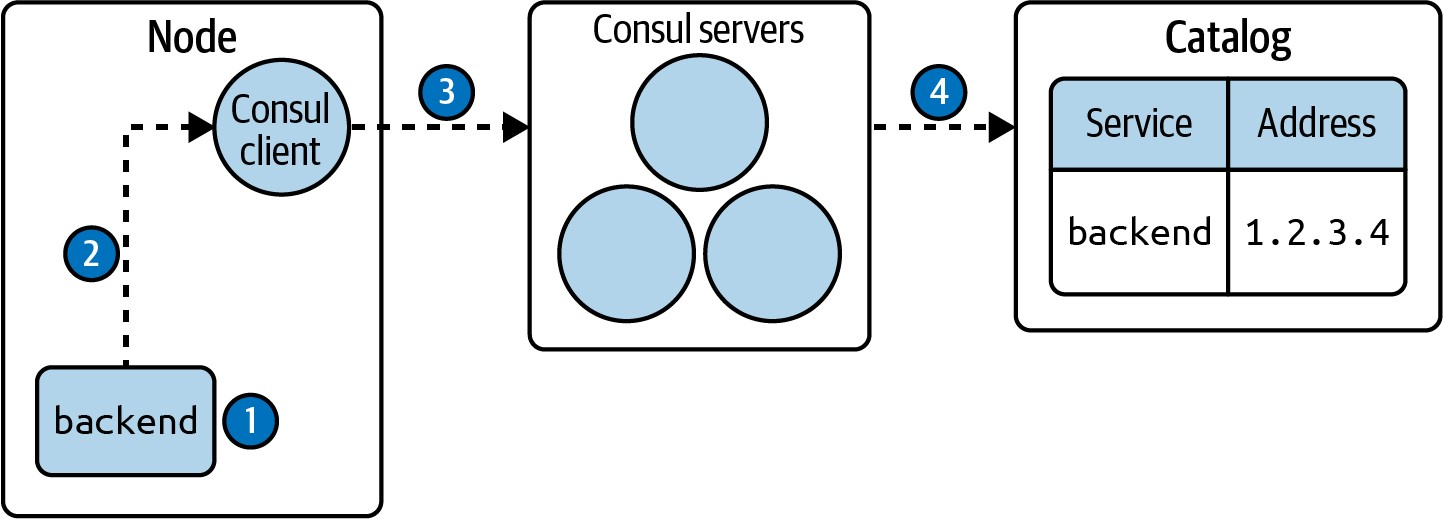
\includegraphics[width=0.7\linewidth]{Pics/example}
		\caption{\label{fig:example} Một dịch vụ mới đang được bắt đầu trên một Node.}
		\label{fig:example}
	\end{figure}

	\hspace{0.3cm}{Consul tự nó không phải là một proxy (Về mặt kỹ thuật, đó là do nó đi kèm với cái được gọi là proxy tích hợp, nhưng proxy này có tối thiểu chức năng và chỉ nên được sử dụng cho các trường hợp thử nghiệm nhỏ) Thay vào đó, Consul sử dụng một proxy gọi là Envoy. Envoy là một proxy nguồn mở được tạo tại Lyft. Nó hiện là một dự án CNCF (Cloud Native Computing Foundation) được nhiều service mesh sử dụng. Envoy được viết bằng C++ cho hiệu năng và có dung lượng bộ nhớ rất thấp. Điều này có nghĩa là nó có thể chạy bên cạnh tất cả các dịch vụ của bạn với tác động tối thiểu đến tài nguyên và độ trễ. Envoy hỗ trợ hàng trăm tính năng để cân bằng tải, khả năng quan sát, kiểm tra sức khỏe, v.v. Máy khách Consul định cấu hình Envoy qua API gRPC của nó.\\}

	
	\hspace{0.3cm}{Trên Kubernetes, sidecar proxy chạy dưới dạng các container riêng biệt trong các nhóm dịch vụ. Điều này đảm bảo rằng các bộ chứa dịch vụ có thể định tuyến đến các proxy sidecar của chúng trong mạng nhóm cục bộ. Trên máy ảo, proxy sidecar chạy dưới dạng các quy trình riêng biệt cho từng phiên bản dịch vụ trên máy ảo đó.\\}
	

	\begin{figure}[h]
		\centering
		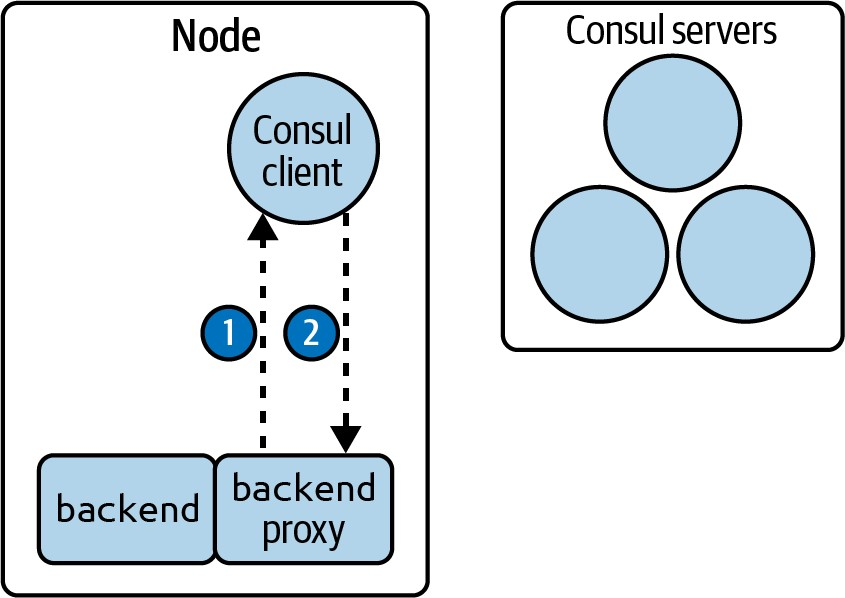
\includegraphics[width=0.7\linewidth]{Pics/example2}
		\caption{\label{fig:example2} Client Consul cấu hình proxy backend.}
		\label{fig:example2}
	\end{figure}

	\hspace{0.3cm}{Bây giờ bạn đã quen thuộc với máy chủ Consul, client và proxy sidecar, hãy xem qua một trường hợp sử dụng ví dụ để hiểu cách cả ba thành phần hoạt động cùng nhau.}
	
	\subsubsection{Trường hợp sử dụng ví dụ}
	\hspace{1cm}{Hãy tưởng tượng một dịch vụ mới gọi là backend được bắt đầu trên một Node (xem bước 1 trong Hình 2.7). Tiếp theo, dịch vụ backend được đăng ký với địa chỉ IP của nó - ví dụ: 1.2.3.4 - vào ứng dụng client Consul trên Node đó (bước 2). Sau đó, ứng dụng client Consul đưa ra yêu cầu quay lại máy chủ Consul để thông báo cho họ biết rằng một dịch vụ mới có tên là backend đang chạy trên Node đó có địa chỉ 1.2.3.4 (bước 3). Các máy chủ Consul sau đó thêm dịch vụ đó vào danh mục (bước 4).\\}
	


	\begin{figure}[p]
		\centering
		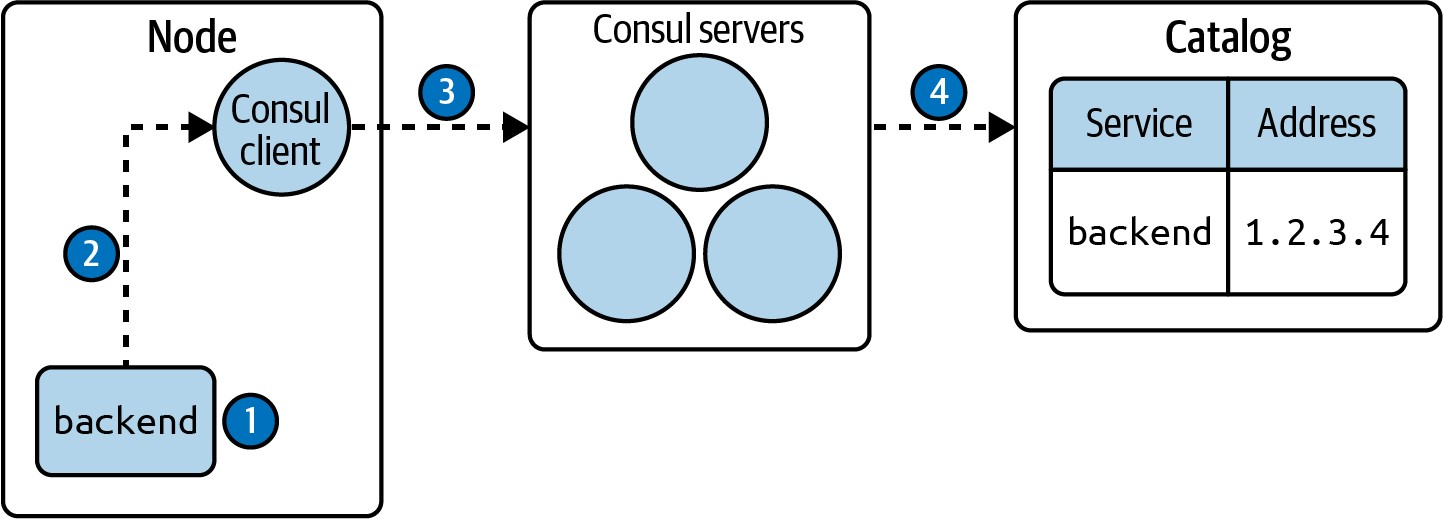
\includegraphics[width=0.7\linewidth]{Pics/example}
		\caption{\label{fig:example} Một dịch vụ mới đang được bắt đầu trên một Node.}
		\label{fig:example}
	\end{figure}
	

	\hspace{0.3cm}{Proxy của giao diện người dùng cần biết địa chỉ của dịch vụ backend để thực hiện yêu cầu. Để thực hiện điều này, ứng dụng client Consul trên cùng một nút với dịch vụ giao diện người dùng sẽ xem danh mục máy chủ Consul để biết các phiên bản mới của dịch vụ backend (bước 1 trong Hình 2.10). Khi một phiên bản mới của dịch vụ backend được đăng ký vào danh mục, máy chủ Consul sẽ gửi địa chỉ mới đến ứng dụng client Consul (bước 2). Sau đó, máy client Consul cập nhật cấu hình proxy của dịch vụ giao diện người dùng với địa chỉ mới cho dịch vụ backend (bước 3).\\}
	


	\hspace{0.3cm}{Đồng thời, proxy cho dịch vụ backend khởi động. Proxy mở một kết nối tới client Consul cục bộ (xem bước 1 hình 2.8). Ứng dụng client Consul định cấu hình proxy và giữ kết nối mở để định cấu hình lại trong tương lai (bước 2).\\}
	
	\begin{figure}[p]

		\centering
		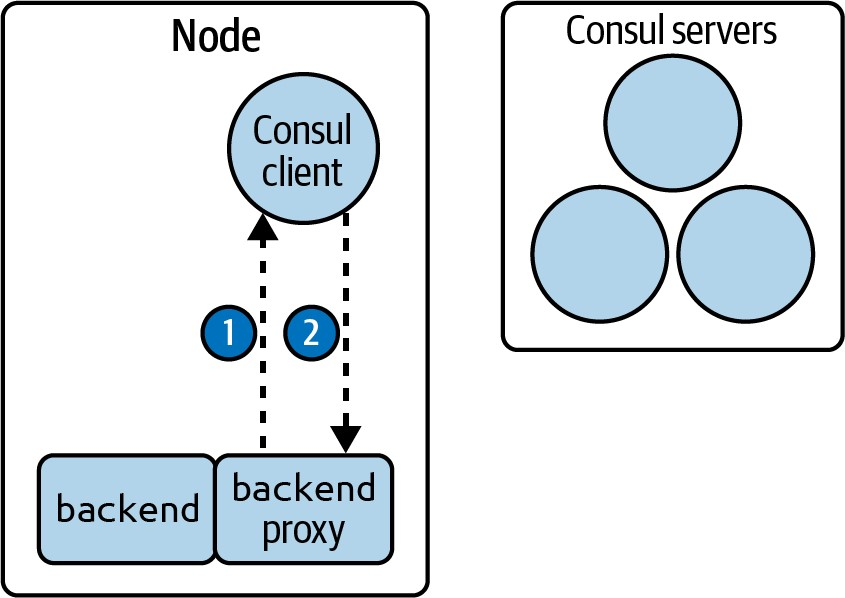
\includegraphics[width=0.7\linewidth]{Pics/example2}
		\caption{\label{fig:example2} Client Consul cấu hình proxy backend.}
		\label{fig:example2}
	\end{figure}
	
	\hspace{0.3cm}{Bây giờ hãy tưởng tượng rằng có một dịch vụ khác gọi là giao diện người dùng đang chạy trên một Node khác trong cụm và dịch vụ giao diện người dùng được cấu hình để giao tiếp với dịch vụ backend (hiển thị trong Hình 2.9).\\}
	
	\begin{figure}[p]
		\centering
		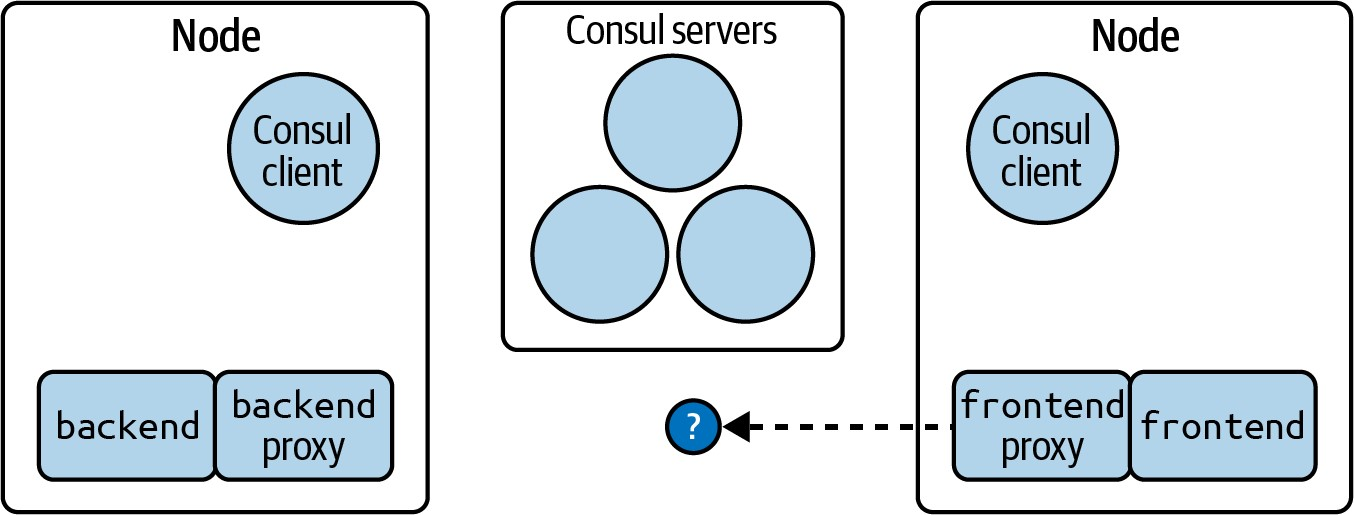
\includegraphics[width=0.7\linewidth]{Pics/example3}
		\caption{\label{fig:example3} Dịch vụ giao diện người dùng được cấu hình để nói chuyện với dịch vụ backend, nhưng nó chưa biết dùng địa chỉ nào.}
		\label{fig:example3}
	\end{figure}
	

	\begin{figure}[h]
		\centering
		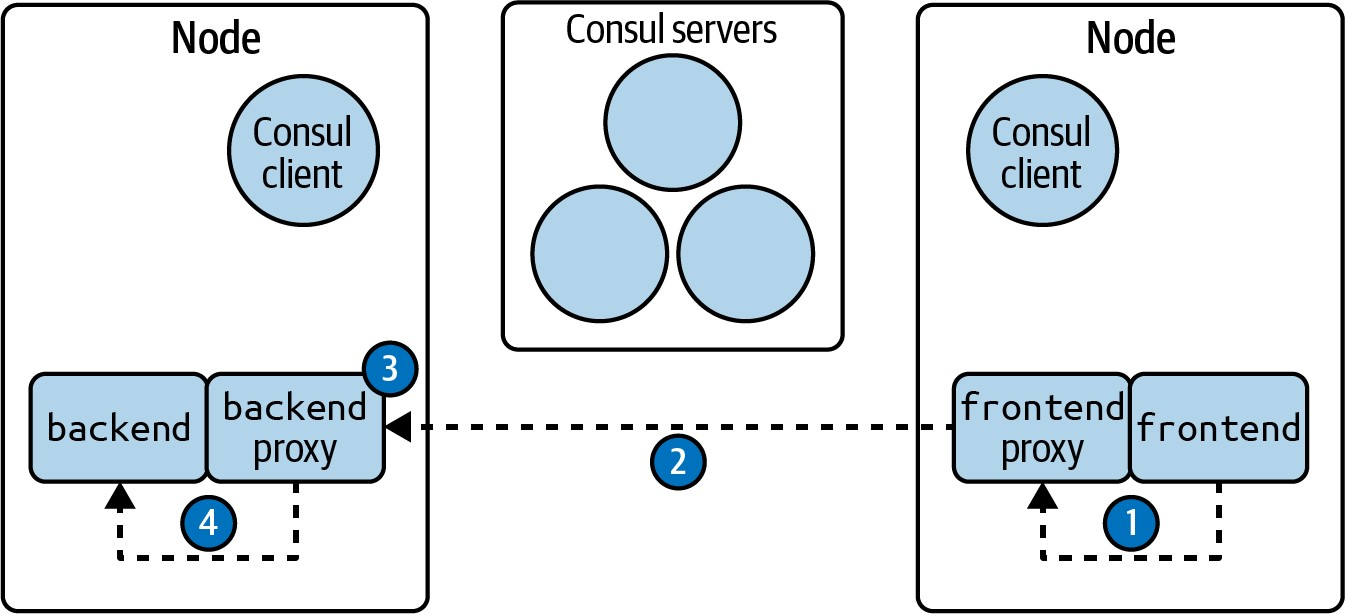
\includegraphics[width=0.7\linewidth]{Pics/example5}
		\caption{\label{fig:example5} Các proxy Sidecar ghi lại lưu lượng trong và ngoài và tuân theo các quy tắc được cấu hình của chúng để hành động trên lưu lượng đó.}
		\label{fig:example5}
	\end{figure}
	
	\hspace{0.3cm}{Ví dụ này minh họa cách máy chủ Consul, client và proxy sidecar hoạt động cùng nhau. Máy chủ Consul và client giao tiếp để chia sẻ dữ liệu về cụm và định cấu hình proxy sidecar. Các proxy Sidecar nắm bắt lưu lượng truy cập vào và ra và tuân theo các quy tắc được định cấu hình của chúng để hành động trên lưu lượng đó, chẳng hạn như bằng cách định tuyến nó tới một proxy khác hoặc không cho phép lưu lượng vì nó không được phép.}
	
	\subsection{Consul so với servece mesh khác}
	\hspace{1cm}{Có nhiều service mesh khác trên thị trường, chẳng hạn như Istio và Linkerd. Hầu hết các mắt service mesh đều tuân theo cùng một kiến trúc chung với một control plane quản lý các proxy sidecar. Consul là duy nhất trong số các mắt lưới khác ở chỗ control plane của nó có thể chạy hoàn toàn tách biệt với Kubernetes. Điều này có nghĩa là nếu bạn đang quản lý một cụm máy ảo thì bạn cũng không cần chạy Kubernetes.\\}
	
	\hspace{0.3cm}{Mỗi service mesh đều có ưu và nhược điểm tùy thuộc vào trường hợp sử dụng chính xác của bạn. Một cách tiếp cận tốt để chọn service mesh là tập trung vào ba trường hợp sử dụng hàng đầu của bạn, chẳng hạn như bảo mật, khả năng quan sát và hỗ trợ đa cụm, sau đó kiểm tra các service mesh phổ biến nhất và chọn một lưới mà bạn cảm thấy phù hợp nhất.}
	
	\subsection{Các tính năng khác của Consul}
	\hspace{1cm}{Consul không chỉ là một mạng service mesh. Đây cũng là kho lưu trữ khóa/giá trị cho cấu hình dịch vụ và giải pháp khám phá dịch vụ DNS. Khi sử dụng DNS, không có proxy sidecar. Các yêu cầu được định tuyến trực tiếp giữa các dịch vụ. Điều này có nghĩa là không có tính năng mã hóa, quan sát hoặc kiểm soát lưu lượng tự động.\\}
	
	\hspace{0.3cm}{Cuốn sách này tập trung vào các tính năng service mesh của Consul, nhưng bạn có thể truy cập tài liệu của Consul để tìm hiểu thêm về các tính năng khác của nó.}
	\section{Bảo mật trong Consul}
	\hspace{1cm}{Trong thế giới ngày nay, an ninh là tối quan trọng. Những kẻ tấn công tinh vi liên tục thăm dò các lỗ hổng có thể dẫn đến việc dữ liệu người dùng bị đánh cắp và hệ thống bị gián đoạn. Những cuộc tấn công này có thể hủy hoại danh tiếng của công ty và tiêu tốn hàng trăm nghìn đô la. Đồng thời, việc bảo vệ chống lại các cuộc tấn công này đang trở nên khó khăn hơn khi việc triển khai microservice ngày càng lớn và phức tạp hơn - do đó làm tăng mục tiêu tấn công của chúng.\\}
	
	\hspace{0.3cm}{Có nhiều khía cạnh để bảo mật hệ thống của bạn và mặc dù service mesh không thể giải quyết tất cả các khía cạnh đó nhưng nó đóng một vai trò quan trọng. Service mesh thực hiện các cải tiến bảo mật thông qua proxy sidecar chặn tất cả lưu lượng truy cập vào và ra khỏi dịch vụ. Một service mesh có thể cung cấp:}
	
	\begin{itemize}
		\item Mã hóa lưu lượng giữa các dịch vụ.
		\item Thực thi các quy tắc về dịch vụ nào có thể giao tiếp với nhau và loại yêu cầu nào được phép - ví dụ: đường dẫn HTTP nào có thể được truy cập.
		\item Một số giảm thiểu chống lại các cuộc tấn công từ chối dịch vụ bằng cách tăng độ tin cậy của dịch vụ.
	\end{itemize}

	\hspace{0.3cm}{Tuy nhiên, vì nó hoạt động ở cấp độ nền tảng nên service mesh không thể cung cấp:}
	
	\begin{itemize}
		\item Tự động vá các thư viện dễ bị tấn công.
		\item Loại bỏ các lỗi bảo mật trong mã code dịch vụ.
		\item Xác thực và ủy quyền người dùng (ví dụ: xác thực mật khẩu).
		\item Phát hiện xâm nhập (Phát hiện xâm nhập đang giám sát hoạt động đáng ngờ. Consul có thể giúp phát hiện xâm nhập vì nó cung cấp số liệu về các yêu cầu bị từ chối. Nếu một dịch vụ đột nhiên có nhiều yêu cầu bị từ chối, có khả năng kẻ tấn công đang cố truy cập dịch vụ đó).
		\item Các cải tiến bảo mật cấp dịch vụ khác.
	\end{itemize}

	\hspace{0.3cm}{Các cải tiến bảo mật mà service mesh cung cấp - mã hóa lưu lượng giữa các dịch vụ và thực thi các quy tắc về dịch vụ nào có thể giao tiếp với nhau - là một phần của việc triển khai mô hình bảo mật được gọi là zero trust network.\\}
	
	\hspace{0.3cm}{Phần này bắt đầu với phần mô tả về mô hình zero trust network và lý do tại sao nó là một cải tiến so với mô hình cũ hơn. Sau đó, trình bày cách Consul triển khai zero trust network và mô tả mã hóa TLS.}
	\subsection{Zero trust network trong Consul}
	\hspace{1cm}{Kiến trúc an ninh mạng truyền thống là theo mô hình castle and moat. Trong mô hình castle and moat, các dịch vụ được triển khai trong một mạng riêng nội bộ (castle - lâu đài) không được kết nối với internet công cộng. Tường lửa (moat - hào nước) bảo vệ quyền truy cập vào mạng nội bộ (Tường lửa là phần mềm hoặc phần cứng kiểm soát quyền truy cập ở rìa mạng - nơi các hệ thống được kết nối với cả mạng riêng và mạng công cộng). Bộ cân bằng tải được triển khai bên ngoài mạng riêng và được phép truy cập thông qua tường lửa. Vì tường lửa đã được đặt sẵn, giả định rằng mọi thứ chạy bên trong mạng nội bộ đều có thể tin cậy được. Vì lý do này, không cần mã hóa, xác thực hoặc ủy quyền giữa các dịch vụ nội bộ.\\}
	
	\begin{figure}[h]
		\centering
		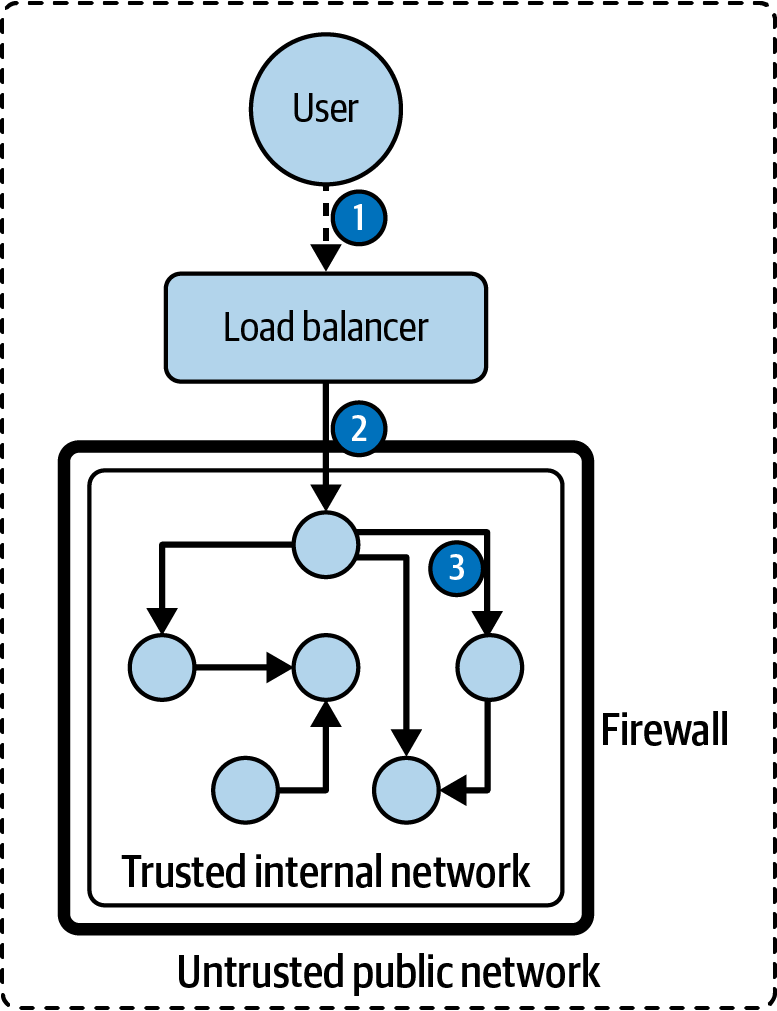
\includegraphics[width=0.5\linewidth]{Pics/castle_and_moat_modal}
		\caption{\label{fig:castleandmoatmodal} Định tuyến bên trong kiến trúc castle and moat.}
		\label{fig:castleandmoatmodal}
	\end{figure}
	
	\hspace{0.3cm}{Hình 2.12 cho thấy lưu lượng truy cập được định tuyến như thế nào qua kiến trúc castle and moat. Ở bước 1, yêu cầu của người dùng được chuyển đến bộ cân bằng tải. Bộ cân bằng tải chuyển tiếp yêu cầu qua tường lửa tới một dịch vụ đang chạy trong mạng nội bộ đáng tin cậy (bước 2). Dịch vụ đó thực hiện cuộc gọi đến các dịch vụ upstream của nó (bước 3). Các cuộc gọi này không được mã hóa và các dịch vụ upstream không kiểm tra ủy quyền vì các cuộc gọi đến từ bên trong mạng nội bộ đáng tin cậy.\\}
	
	\hspace{0.3cm}{Vấn đề với mô hình castle and moat là những kẻ tấn công giành được quyền truy cập vào toàn bộ hệ thống nếu chúng xâm phạm bất kỳ điểm nào trong mạng nội bộ, như trong Hình 2.13. Điều này có nghĩa là bảo mật của hệ thống chỉ tốt bằng liên kết yếu nhất của nó.\\}
	
	\begin{figure}[h]
		\centering
		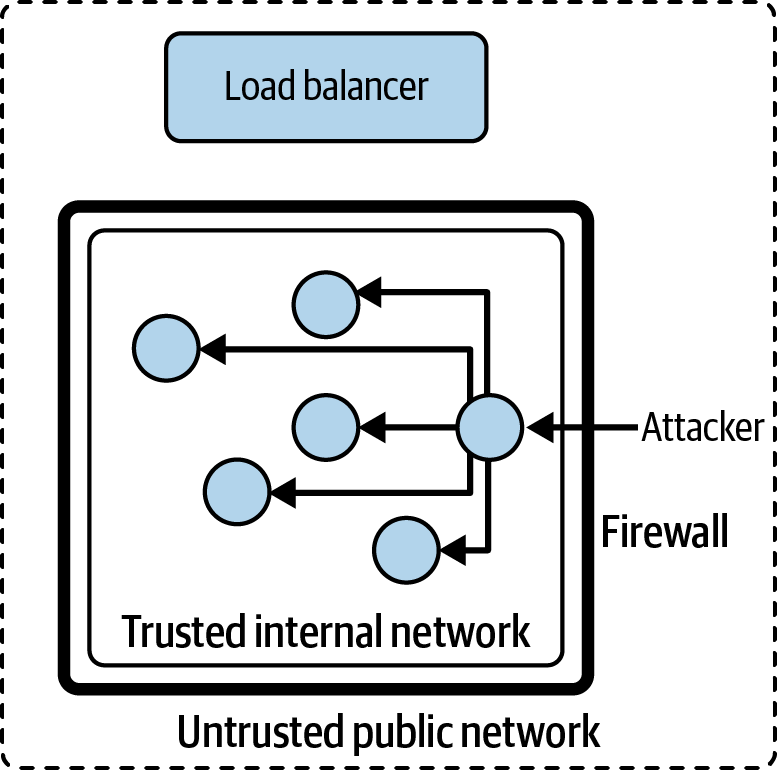
\includegraphics[width=0.5\linewidth]{Pics/threat_of_castle_and_moat}
		\caption{\label{fig:threatofcastleandmoat} Trong kiến trúc castle and moat, nếu kẻ tấn công xâm phạm một dịch vụ, chúng có thể yêu cầu tất cả các dịch vụ và cơ sở dữ liệu bên trong mạng.}
		\label{fig:threatofcastleandmoat}
	\end{figure}
	
	\hspace{0.3cm}{Đây không phải là một điểm yếu lý thuyết. Vào năm 2015, tin tặc đã đánh cắp hàng triệu hồ sơ nhạy cảm về nhân viên chính phủ từ Văn phòng Quản lý Nhân sự Hoa Kỳ (OPM). Những kẻ tấn công đã giành được quyền truy cập bằng cách xâm nhập vào hệ thống của một công ty hợp đồng có máy chủ có toàn quyền truy cập vào mạng OPM. Từ đó, họ có thể tự do trích xuất dữ liệu từ các máy chủ OPM.\\}
	
	\hspace{0.3cm}{Điểm yếu của hệ thống castle and moat là không thể chấp nhận được đối với hầu hết các công ty, vì vậy các kỹ sư bảo mật đề xuất một mô hình khác: zero trust network.\\}
	
	\hspace{0.3cm}{Trong zero trust network, bạn cho rằng mạng nội bộ bị xâm phạm. Do đó, các dịch vụ không hoàn toàn tin tưởng các yêu cầu đơn giản chỉ vì chúng đến từ bên trong mạng nội bộ. Thay vào đó, các dịch vụ thực hiện mã hóa, xác thực và ủy quyền cho tất cả các yêu cầu.}
	
	\subsubsection{Mã hóa}
	\hspace{1cm}{Quá trình sửa đổi dữ liệu sao cho bên thứ ba không thể đọc dữ liệu gốc chưa sửa đổi, nhưng người nhận thì có thể. Trong mạng máy tính, quy trình mã hóa TLS thường được sử dụng để đảm bảo rằng các bên thứ ba không thể chặn và đọc dữ liệu được gửi giữa người dùng và trang web mà họ đang xem. TLS được sử dụng bí mật khi bạn truy cập các trang web https://.}
	
	\subsubsection{Xác thực}
	\hspace{1cm}{Quá trình xác thực rằng một thực thể là người đã được xác minh, công nhận. Ví dụ: nếu người dùng tuyên bố là người dùng quản trị, thì xác thực là quá trình kiểm tra xem mật khẩu họ cung cấp có khớp với mật khẩu dự kiến hay không. Sau khi một thực thể được xác thực, bạn vẫn cần kiểm tra xem họ có được phép thực hiện hành động mà họ đang cố thực hiện hay không.}
	
	\subsubsection{Ủy quyền}
	\hspace{1cm}{Quá trình xác thực rằng một thực thể được xác thực được phép thực hiện một hành động cụ thể nào đó hay không. Ví dụ: người dùng đã đăng nhập có thể được xác thực nhưng có lẽ họ không được phép xem bảng quản trị.}

	\subsection{Mã hóa trong Consul}
	\hspace{1cm}{Mã hóa là cần thiết trong mạng zero trust network vì dịch vụ bị xâm phạm có thể đọc lưu lượng được truyền giữa các dịch vụ khác- điều này được gọi là traffic sniffng hoặc tấn công trung gian (xem Hình 2.14). (Có nhiều cơ chế để một dịch vụ bị xâm nhập chặn bắt lưu lượng truy cập. Nếu dịch vụ bị xâm nhập nằm trên cùng một node với một dịch vụ khác, dịch vụ đó có thể có quyền kiểm tra lưu lượng mạng của các quy trình khác. Hoặc một dịch vụ bị xâm phạm có thể sử dụng một kỹ thuật gọi là giả mạo Giao thức phân giải địa chỉ (ARP) để khiến một dịch vụ khác gửi nhầm lưu lượng truy cập của nó đến dịch vụ bị xâm phạm thay vì đích dự kiến).\\}
	
	\begin{figure}[h]
		\centering
		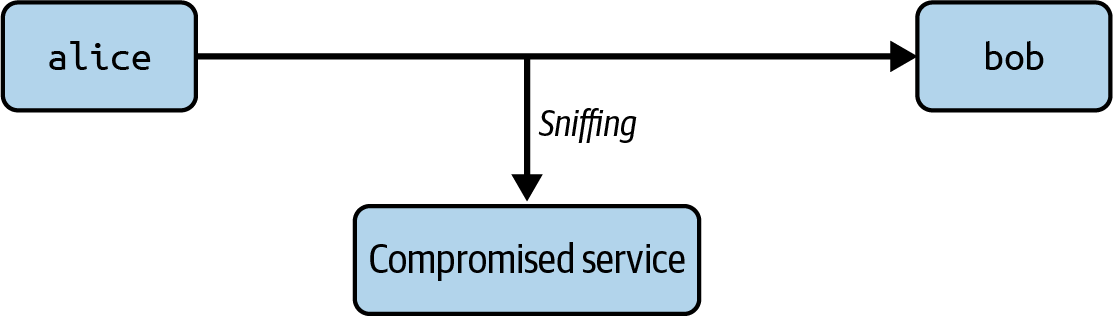
\includegraphics[width=0.7\linewidth]{Pics/sniffing}
		\caption{\label{fig:sniffing} Một dịch vụ bị xâm nhập có thể chặn truy tìm được gửi giữa hai dịch vụ khác.}
		\label{fig:sniffing}
	\end{figure}
	
	\hspace{0.3cm}{Mã hóa ngăn chặn các cuộc tấn công trung gian vì những kẻ tấn công không thể đọc dữ liệu được gửi giữa hai dịch vụ. Chỉ dịch vụ đích mới có thể giải mã dữ liệu. Như thể hiện trong Hình 2.13, nếu Bob là dịch vụ duy nhất có khả năng giải mã lưu lượng truy cập từ dịch vụ Alice, thì việc kẻ tấn công chặn lưu lượng cũng không thành vấn đề.\\}
	
	\begin{figure}[h]
		\centering
		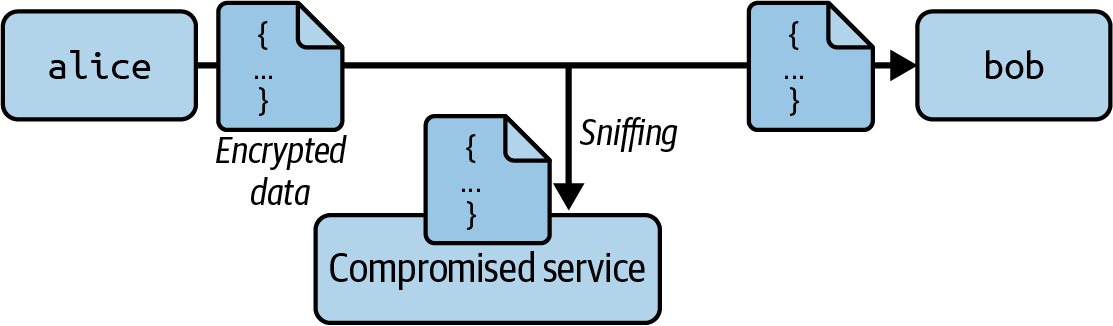
\includegraphics[width=0.7\linewidth]{Pics/encrypt_prevent_sniffing}
		\caption{\label{fig:encryptpreventsniffing} Dữ liệu điện tử hiện đã được mã hóa, do đó, ngay cả khi dịch vụ bị xâm phạm sniffing, chúng cũng không thể lấy được nội dung gốc.}
		\label{fig:encryptpreventsniffing}
	\end{figure}
	
	\hspace{0.3cm}{Consul sử dụng mã hóa TLS để mã hóa lưu lượng giữa các dịch vụ.}
	
	\subsubsection{Mã hóa TLS}
	\hspace{1cm}{Mã hóa TLS có ba bước (xem Hình 2.16 để biết minh họa):}
	\begin{enumerate}
	\item Dịch vụ nguồn và đích đồng ý về khóa mã hóa.
	\item Dịch vụ nguồn mã hóa tin nhắn của nó bằng khóa đã thỏa thuận và gửi tin nhắn được mã hóa đến dịch vụ đích.
	\item Dịch vụ đích giải mã tin nhắn bằng khóa đã thỏa thuận.
	\end{enumerate}

	\begin{figure}[h]
		\centering
		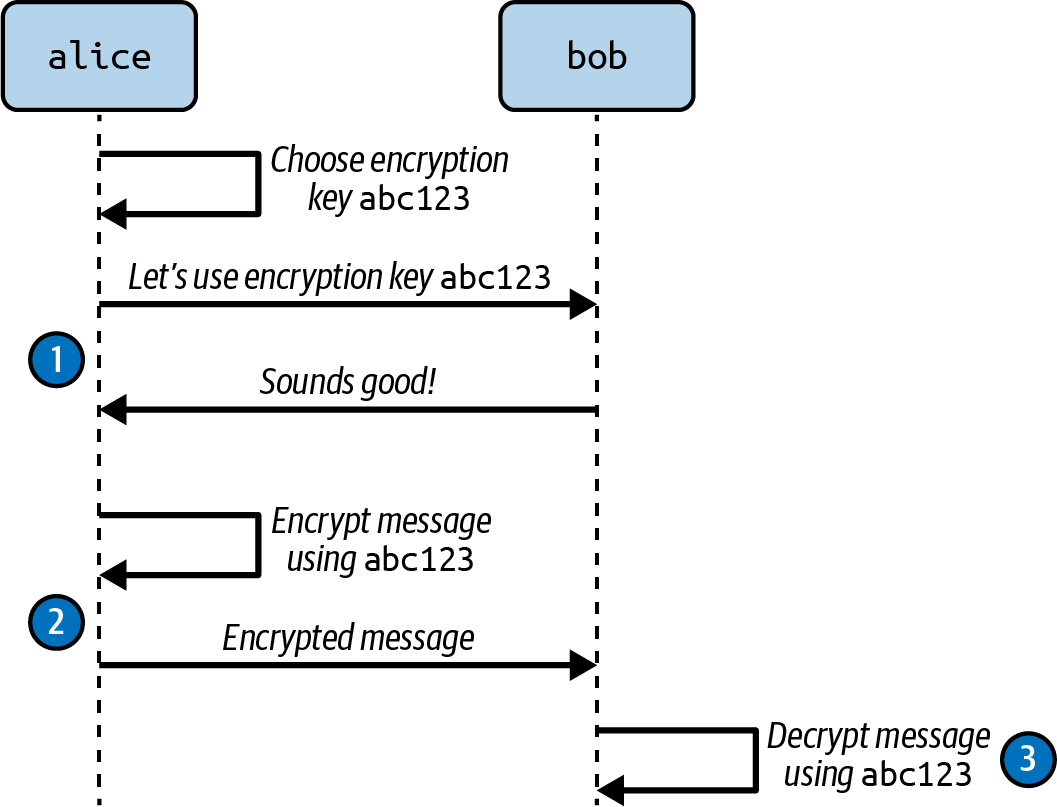
\includegraphics[width=0.7\linewidth]{Pics/TLS}
		\caption{\label{fig:tls} Một minh họa về mã hóa TLS.}
		\label{fig:tls}
	\end{figure}
	
	\hspace{0.3cm}{Miễn là những kẻ tấn công trung gian không biết khóa mã hóa, chúng không thể giải mã tin nhắn. Loại mã hóa này được gọi là mã hóa đối xứng vì cả hai bên đều biết khóa mã hóa.\\}
	
	\hspace{0.3cm}{Nhưng làm thế nào để khóa mã hóa đối xứng được thỏa thuận mà không có kẻ tấn công chặn nó? Đây là lúc mật mã khóa công khai phát huy tác dụng.\\}
	
	\hspace{0.3cm}{Mật mã khóa công khai là một phương pháp mã hóa sử dụng các cặp khóa: khóa bí mật và khóa công khai. Các khóa được liên kết về mặt toán học sao cho các thông báo được mã hóa bằng khóa công khai chỉ có thể được giải mã bằng khóa bí mật. Mật mã khóa công khai cho phép cả hai dịch vụ đồng ý với khóa mã hóa đối xứng mà khóa đó không được gửi qua mạng, nơi khóa có thể bị đánh cắp.\\}
	
	\hspace{0.3cm}{Hãy xem qua một ví dụ sử dụng hai dịch vụ tưởng tượng, Alice và Bob, muốn đồng ý về một khóa mã hóa đối xứng:}
	
	\begin{enumerate}
	\item Dịch vụ Alice tạo hai khóa, một khóa bí mật có tên alice-priv và một khóa công khai có tên alice-pub.
	\item Dịch vụ Alice gửi khóa công khai của nó - alice-pub đến dịch vụ Bob. Khóa được gửi dưới dạng văn bản rõ để kẻ tấn công có thể nhìn thấy khóa.
	\item Dịch vụ Bob cũng làm như vậy. Nó tạo ra hai khóa, bob-priv và bob-pub, đồng thời gửi khóa bob-pub cho Alice. Một lần nữa, kẻ tấn công có thể thấy khóa bob-pub.
	\item Ngay bây giờ Alice sẵn sàng gửi khóa mã hóa đối xứng cho Bob. Alice mã hóa khóa mã hóa đối xứng bằng khóa công khai của Bob - bob-pub.
	\item Alice gửi thông điệp được mã hóa này cho Bob. Một lần nữa, kẻ tấn công có thể nhìn thấy thông điệp được mã hóa này, nhưng điều kỳ diệu của mật mã khóa công khai là kẻ tấn công không thể giải mã thông điệp bằng các khóa công khai alice-pub hoặc bob-pub. Thuật toán sử dụng để mã hóa thông điệp được thiết kế sao cho chỉ khóa bí mật của Bob (bob-priv) mới có thể giải mã nó.
	\item Bob nhận được thông điệp được mã hóa và sử dụng khóa riêng của nó - bob-priv để giải mã.
	\item Giờ đây, khóa mã hóa đối xứng đã được thỏa thuận một cách an toàn, Alice và Bob có thể tự do gửi thêm thông điệp bằng cách mã hóa chúng khóa mã hóa đối xứng.
	\end{enumerate}

	\begin{figure}[h]
		\centering
		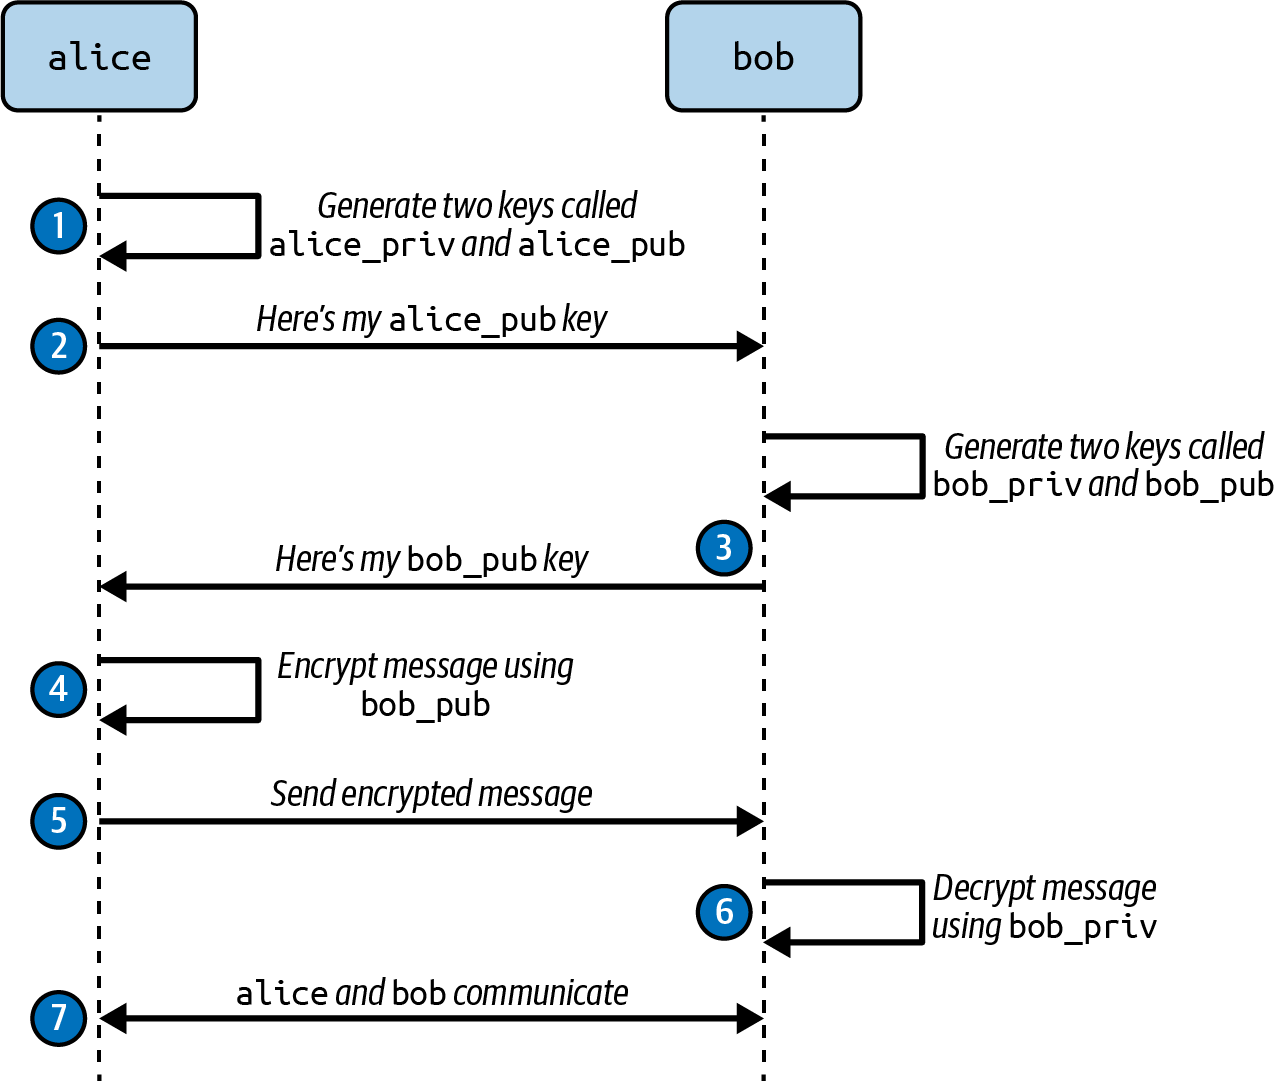
\includegraphics[width=0.7\linewidth]{Pics/public-key_cryptography}
		\caption{\label{fig:public-keycryptography} Sơ đồ mật mã khóa công khai.}
		\label{fig:public-keycryptography}
	\end{figure}
	
	\hspace{0.3cm}{Vì lý do hiệu suất, mật mã khóa công khai chỉ được sử dụng khi bắt đầu kết nối TLS để đồng ý một cách an toàn về khóa mã hóa đối xứng. Từ đó trở đi, khóa mã hóa đối xứng đó được sử dụng để mã hóa tất cả dữ liệu được gửi giữa hai dịch vụ.\\}
	
	\hspace{0.3cm}{Đó chính là cách hoạt động của mã hóa TLS, Consul sử dụng TLS để mã hóa lưu lượng service mesh.}
	
	\subsubsection{Mã hóa trong Consul}
	\hspace{1cm}{Mã hóa TLS trong Consul được bật theo mặc định. Khi một dịch vụ đưa ra yêu cầu thông qua proxy sidecar của nó, proxy sẽ tự động mã hóa yêu cầu đó bằng TLS. Dịch vụ có thể tiếp tục thực hiện các yêu cầu không được mã hóa và proxy đảm bảo các yêu cầu đó được mã hóa trước khi chúng rời khỏi mạng cục bộ.\\}
	
	\hspace{0.3cm}{Quá trình này được thể hiện trong Hình 2.18. Ở bước 1, Consul cung cấp khóa công khai và khóa bí mật cho từng proxy. Khi giao diện người dùng gửi một yêu cầu không được mã hóa đến chương trình backend, thì yêu cầu đó sẽ bị chặn bởi proxy của giao diện người dùng (bước 2) và mã hóa yêu cầu đó trước khi chuyển tiếp đến chương trình backend (bước 3). Ở phía bên nhận, proxy của chương trình backend sẽ chặn yêu cầu (bước 4) và giải mã nó trước khi chuyển tiếp đến dịch vụ đích (bước 5).\\}
	
	\begin{figure}
		\centering
		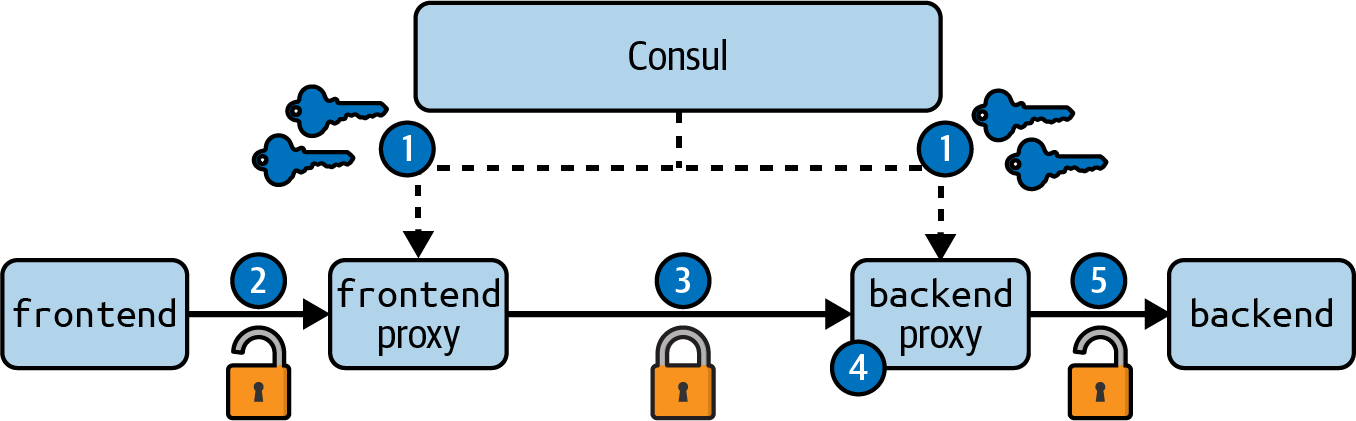
\includegraphics[width=0.7\linewidth]{Pics/Sidecar_proxies_automatically_encrypt}
		\caption{\label{fig:sidecarproxiesautomaticallyencrypt} Sidecar proxy tự động mã hóa lưu lượng bằng TLS.}
		\label{fig:sidecarproxiesautomaticallyencrypt}
	\end{figure}
	
	\hspace{0.3cm}{Với cơ chế này, các dịch vụ không cần phải sửa đổi để sử dụng TLS - tất cả đều diễn ra tự động mà chúng không hề hay biết.\\}
	
	\hspace{0.3cm}{Đó chính xác là cách Consul thực hiện mã hóa. Mã hóa là điều cần thiết trong một zero trust network, nhưng nó vẫn không đủ. Nếu không có xác thực và ủy quyền, một dịch vụ bị xâm phạm vẫn có thể thực hiện các yêu cầu thông qua proxy sidecar của nó tới bất kỳ dịch vụ nào trong mạng.}
	
	\subsection{Xác thực trong Consul}
	\hspace{1cm}{Xác thực là quá trình xác minh rằng ai đó là người mà đã được xác minh; đó là về việc xác minh danh tính. Trong mạng dịch vụ, điều này có hai phần: dịch vụ nguồn phải xác minh rằng dịch vụ đích thực sự là dịch vụ mà nó muốn giao tiếp và dịch vụ đích phải xác minh rằng dịch vụ nguồn thực sự là dịch vụ mà nó yêu cầu.\\}
	
	\hspace{0.3cm}{Cụ thể, nếu giao diện người dùng đang gọi phần backend, thì giao diện người dùng cần đảm bảo rằng nó thực sự đang nói chuyện với phần backend. Nếu nó không kiểm tra, thì nó có thể đang gửi yêu cầu của mình tới kẻ tấn công. Backend cũng cần xác minh dịch vụ nào đang thực hiện yêu cầu để có thể kiểm tra xem dịch vụ đó có được phép giao tiếp với nó hay không.\\}
	
	\hspace{0.3cm}{Consul cũng tận dụng TLS để thực hiện xác thực. Khi các dịch vụ trao đổi khóa công khai của họ, họ thực sự trao đổi chứng chỉ. Chứng chỉ này chứa khóa công khai và thông tin về dịch vụ, chẳng hạn như ID của nó.\\}
	
	\hspace{0.3cm}{Đây là các bước liên quan đến xác thực TLS (xem Hình 2.19 để minh họa):}
	
	\begin{enumerate}
	\item Consul cấp chứng chỉ công khai và khóa bí mật cho từng dịch vụ. Được mã hóa trong chứng chỉ công khai là ID của dịch vụ đó.
	\item Trong quá trình trao đổi khóa, chứng chỉ công khai cho mỗi dịch vụ được trao đổi.
	\item Mỗi dịch vụ kiểm tra chứng chỉ công khai của dịch vụ kia và đảm bảo rằng ID dịch vụ là những gì được mong đợi. Ví dụ: dịch vụ giao diện người dùng sẽ xác minh rằng chứng chỉ dành cho dịch vụ backend và dịch vụ backend sẽ xác minh rằng chứng chỉ dành cho dịch vụ giao diện người dùng.
	\item Nếu danh tính được xác minh, yêu cầu sẽ tiếp tục.
	\end{enumerate}

	\begin{figure}[h]
		\centering
		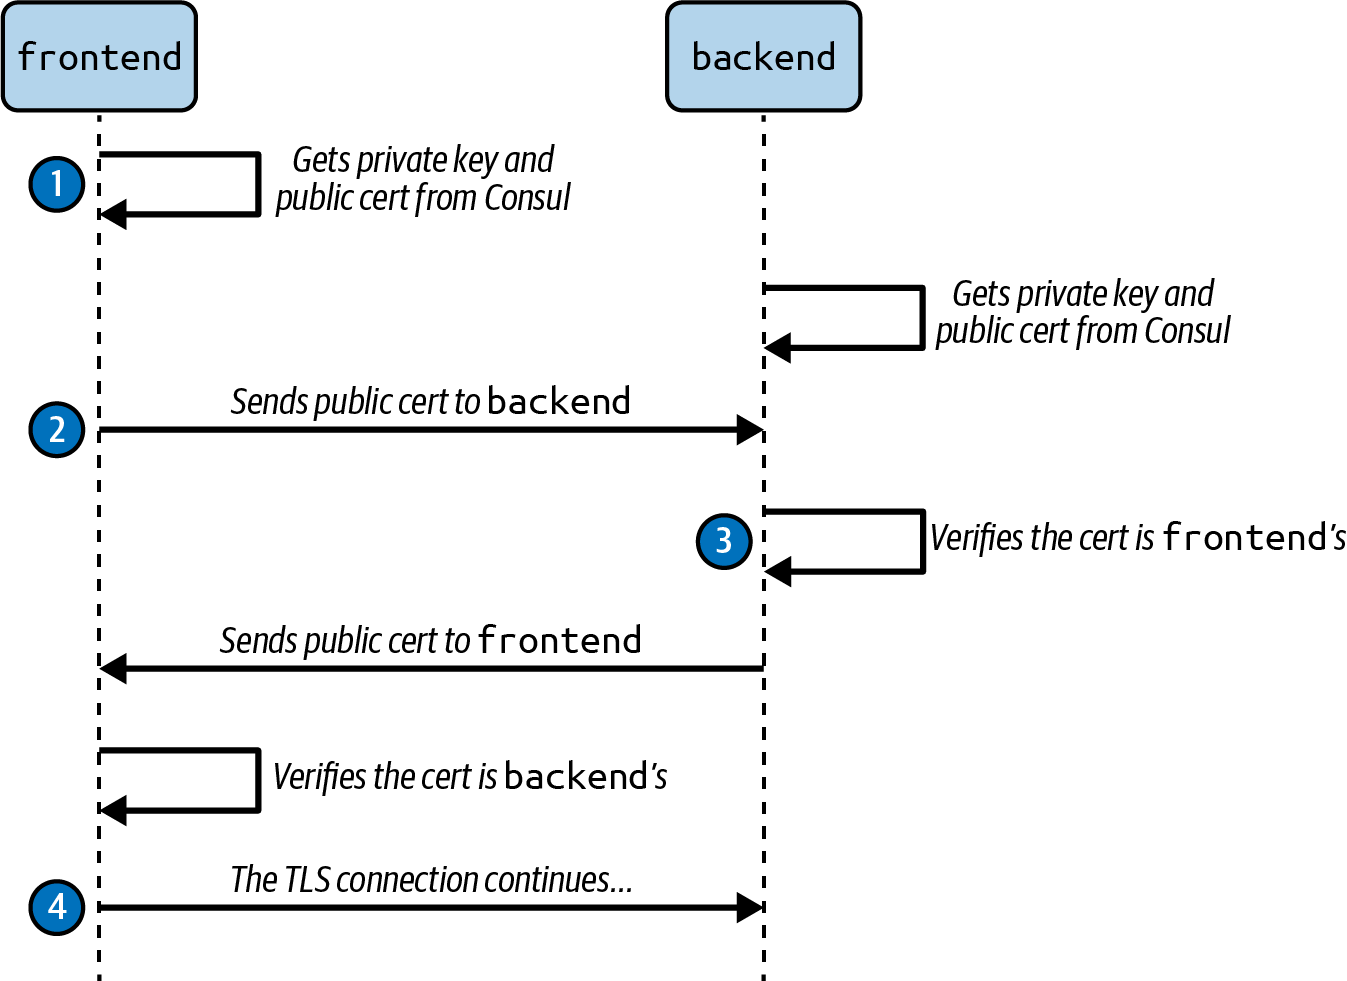
\includegraphics[width=0.7\linewidth]{Pics/TLS_provide_authentication}
		\caption{\label{fig:tlsprovideauthentication} TLS được sử dụng để cung cấp xác thực.}
		\label{fig:tlsprovideauthentication}
	\end{figure}
	
	\hspace{0.3cm}{Chúng ta có thể tự hỏi điều gì ngăn kẻ tấn công tạo chứng chỉ công khai của riêng chúng để mạo danh bất kỳ dịch vụ nào. Để ngăn chặn điều này, Consul hoạt động như một cơ quan cấp chứng chỉ.\\}
	
	\hspace{0.3cm}{Cơ quan cấp chứng chỉ là một thực thể cấp chứng chỉ được ký bằng mật mã sao cho chúng chỉ có thể đến từ cơ quan cấp chứng chỉ đó. Cơ quan cấp chứng chỉ cũng có chứng chỉ công khai được gọi là chứng chỉ của cơ quan cấp chứng chỉ (chứng chỉ CA). Khi xuất trình chứng chỉ công khai của dịch vụ - ví dụ: chứng chỉ backend - bên thứ ba có thể sử dụng chứng chỉ CA để kiểm tra xem chứng chỉ công khai có được ký bởi cơ quan cấp chứng chỉ đó hay không.\\}
	
	\hspace{0.3cm}{Cụ thể, ngoài chứng chỉ công khai và khóa bí mật mà Consul cấp cho từng dịch vụ, Consul còn cấp cho từng dịch vụ chứng chỉ CA của mình. Sau đó, chứng chỉ CA này có thể được sử dụng để xác minh rằng Consul thực sự đã cấp chứng chỉ công khai và việc tin cậy ID dịch vụ được mã hóa bên trong là an toàn.\\}
	
	\begin{figure}[h]
		\centering
		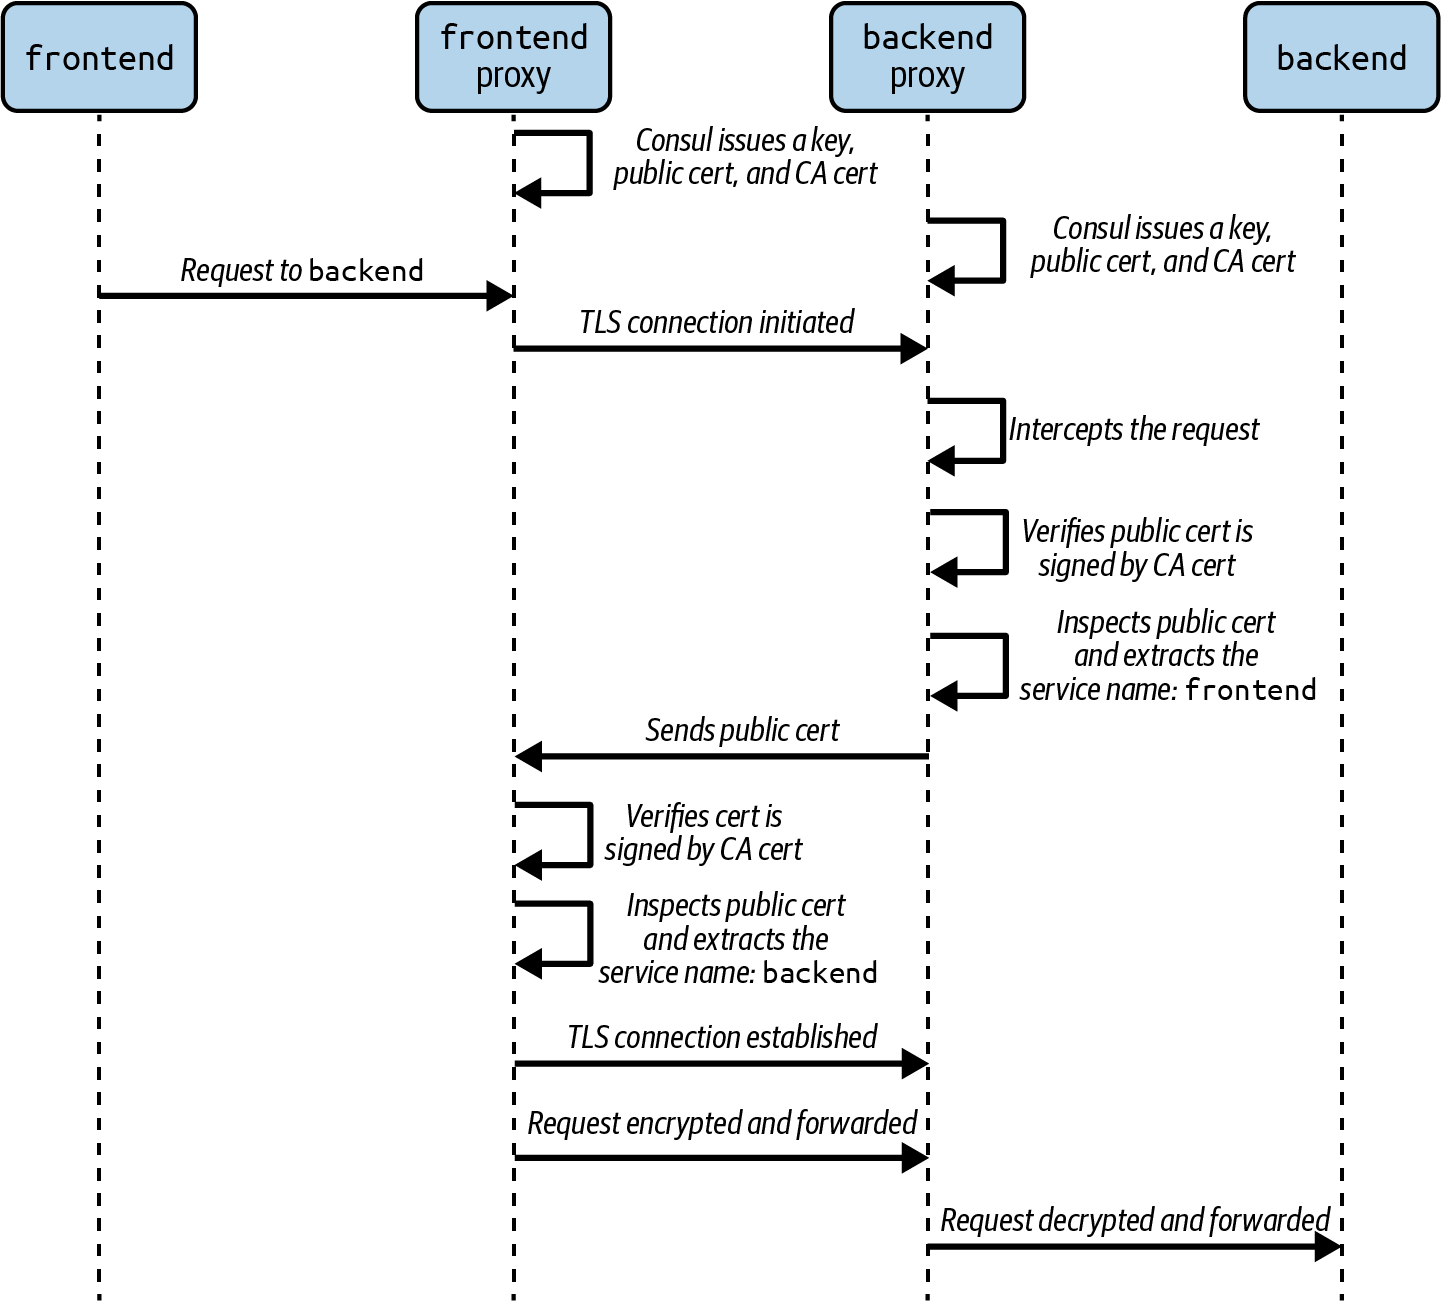
\includegraphics[width=0.7\linewidth]{Pics/frontend_talk_to_backend_securely}
		\caption{\label{fig:frontendtalktobackendsecurely} Quy trình khi giao diện người dùng giao tiếp với phần backend một cách an toàn.}
		\label{fig:frontendtalktobackendsecurely}
	\end{figure}
	
	\hspace{0.3cm}{Bạn có thể xem các chứng chỉ công khai của từng dịch vụ bằng công cụ openssl.}
	\subsection{Ủy quyền trong Consul}
	\hspace{1cm}{Ủy quyền là quá trình xác định xem một thực thể được xác thực có được phép thực hiện một hành động nhất định hay không. Ví dụ: dịch vụ này có được phép thực hiện các yêu cầu đối với dịch vụ đó hay được phép truy cập vào một đường dẫn HTTP cụ thể không?\\}
	
	\hspace{0.3cm}{Consul thực hiện ủy quyền thông qua hệ thống chủ đích của nó. Chủ đích là các quy tắc chi phối các dịch vụ nào được phép giao tiếp.\\}
	
	\hspace{0.3cm}{Mọi chủ đích đều có nguồn gốc và đích đến. Ví dụ: một chủ đích có thể cho phép một giao diện người dùng dịch vụ cụ thể (nguồn) kết nối với một dịch vụ backend cụ thể (đích). Ngoài ra, ký tự đại diện có thể được sử dụng làm nguồn hoặc đích, chẳng hạn như cho phép một cổng vào kết nối với bất kỳ dịch vụ nào hoặc bất kỳ dịch vụ nào kết nối với bất kỳ dịch vụ nào khác.\\}
	
	\hspace{0.3cm}{Ngoài việc chỉ định các quy tắc dựa trên dịch vụ nguồn và đích, bạn có thể sử dụng các chủ đích để kiểm soát các phương thức, đường dẫn và tiêu đề HTTP hoặc gRPC nào được ủy quyền. Consul gọi những chủ đích này là nhận biết ứng dụng vì chúng liên quan đến cách ứng dụng thực sự hoạt động. Ví dụ: bạn có thể tạo một chủ đích cho phép cổng vào truy cập vào bất kỳ đường dẫn nào trên dịch vụ giao diện người dùng ngoại trừ /admin.\\}
	
	\hspace{0.3cm}{Cơ chế thực thi chủ đích như sau:}
	
	\begin{enumerate}
	\item Dịch vụ nguồn gửi yêu cầu đến dịch vụ đích.
	\item Proxy của dịch vụ đích xác minh chứng chỉ công khai của dịch vụ nguồn và trích xuất tên dịch vụ từ ID.
	\item Proxy của dịch vụ đích kiểm tra danh sách các chủ đích của nó để đảm bảo rằng dịch vụ nguồn được phép thực hiện kết nối.
	\item Nếu đã đặt chủ đích nhận biết ứng dụng, proxy của dịch vụ đích cũng xác minh rằng yêu cầu cụ thể đó được cho phép.
	\end{enumerate}

	\hspace{0.3cm}{Proxy của giao diện người dùng cần biết địa chỉ của dịch vụ backend để thực hiện yêu cầu. Để thực hiện điều này, ứng dụng client Consul trên cùng một nút với dịch vụ giao diện người dùng sẽ xem danh mục máy chủ Consul để biết các phiên bản mới của dịch vụ backend (bước 1 trong Hình 2.10). Khi một phiên bản mới của dịch vụ backend được đăng ký vào danh mục, máy chủ Consul sẽ gửi địa chỉ mới đến ứng dụng client Consul (bước 2). Sau đó, máy client Consul cập nhật cấu hình proxy của dịch vụ giao diện người dùng với địa chỉ mới cho dịch vụ backend (bước 3).\\}
	
	\begin{figure}[p]
		\centering
		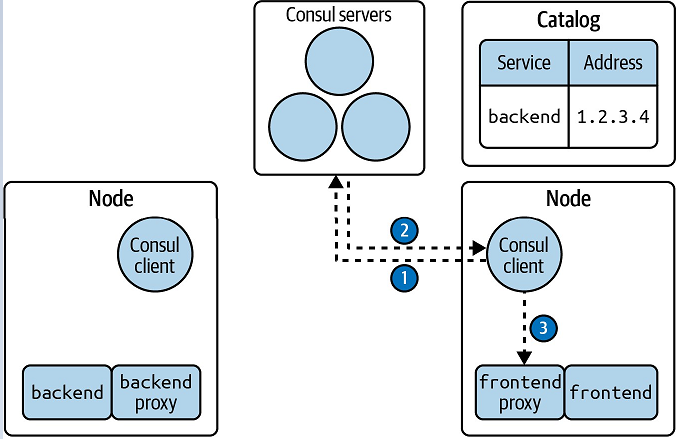
\includegraphics[width=0.7\linewidth]{Pics/example4}
		\caption{\label{fig:example4} Proxy của giao diện người dùng học địa chỉ của dịch vụ backend để thực hiện yêu cầu.}
		\label{fig:example4}
	\end{figure}
	
	\hspace{0.3cm}{Bây giờ proxy của dịch vụ giao diện người dùng biết địa chỉ của dịch vụ backend. Khi dịch vụ giao diện người dùng đưa ra yêu cầu của nó, proxy của giao diện người dùng sẽ chặn nó (bước 1 trong Hình 2.11). Proxy thấy rằng yêu cầu bị ràng buộc đối với dịch vụ backend và vì nó biết địa chỉ của dịch vụ backend, 1.2.3.4, nên nó sẽ chuyển tiếp yêu cầu đến địa chỉ đó (bước 2). Yêu cầu đến dịch vụ backend, nơi proxy của dịch vụ backend chặn nó (bước 3). Giả sử rằng proxy của backend được định cấu hình để chỉ cho phép các yêu cầu từ dịch vụ giao diện người dùng. Proxy kiểm tra yêu cầu và thấy rằng đó là từ dịch vụ giao diện người dùng, và do đó, nó cho phép yêu cầu thông qua (bước 4).\\}
	
	\begin{figure}[p]
		\centering
		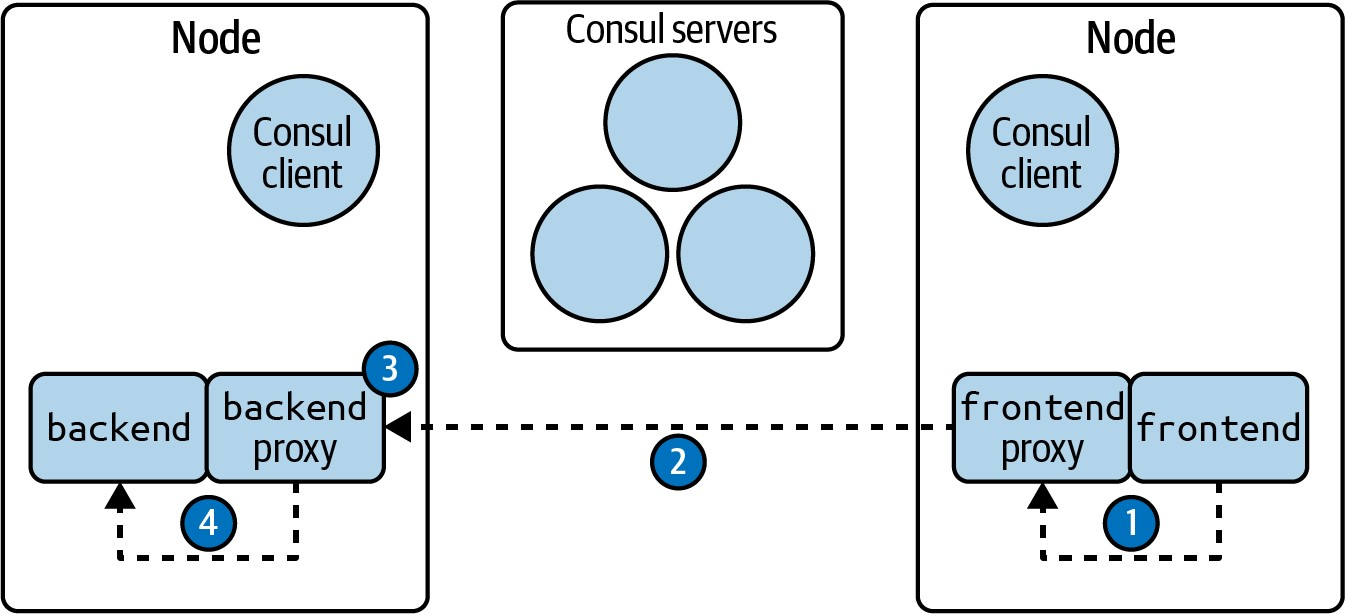
\includegraphics[width=0.7\linewidth]{Pics/example5}
		\caption{\label{fig:example5} Các proxy Sidecar ghi lại lưu lượng trong và ngoài và tuân theo các quy tắc được cấu hình của chúng để hành động trên lưu lượng đó.}
		\label{fig:example5}
	\end{figure}
	
	\hspace{0.3cm}{Ví dụ này minh họa cách máy chủ Consul, client và proxy sidecar hoạt động cùng nhau. Máy chủ Consul và client giao tiếp để chia sẻ dữ liệu về cụm và định cấu hình proxy sidecar. Các proxy Sidecar nắm bắt lưu lượng truy cập vào và ra và tuân theo các quy tắc được định cấu hình của chúng để hành động trên lưu lượng đó, chẳng hạn như bằng cách định tuyến nó tới một proxy khác hoặc không cho phép lưu lượng vì nó không được phép.}
	
	\subsection{Consul so với servece mesh khác}
	\hspace{1cm}{Có nhiều service mesh khác trên thị trường, chẳng hạn như Istio và Linkerd. Hầu hết các mắt service mesh đều tuân theo cùng một kiến trúc chung với một control plane quản lý các proxy sidecar. Consul là duy nhất trong số các mắt lưới khác ở chỗ control plane của nó có thể chạy hoàn toàn tách biệt với Kubernetes. Điều này có nghĩa là nếu bạn đang quản lý một cụm máy ảo thì bạn cũng không cần chạy Kubernetes.\\}
	
	\hspace{0.3cm}{Mỗi service mesh đều có ưu và nhược điểm tùy thuộc vào trường hợp sử dụng chính xác của bạn. Một cách tiếp cận tốt để chọn service mesh là tập trung vào ba trường hợp sử dụng hàng đầu của bạn, chẳng hạn như bảo mật, khả năng quan sát và hỗ trợ đa cụm, sau đó kiểm tra các service mesh phổ biến nhất và chọn một lưới mà bạn cảm thấy phù hợp nhất.}
	
	\subsection{Các tính năng khác của Consul}
	\hspace{1cm}{Consul không chỉ là một mạng service mesh. Đây cũng là kho lưu trữ khóa/giá trị cho cấu hình dịch vụ và giải pháp khám phá dịch vụ DNS. Khi sử dụng DNS, không có proxy sidecar. Các yêu cầu được định tuyến trực tiếp giữa các dịch vụ. Điều này có nghĩa là không có tính năng mã hóa, quan sát hoặc kiểm soát lưu lượng tự động.\\}
	
	\hspace{0.3cm}{Cuốn sách này tập trung vào các tính năng service mesh của Consul, nhưng bạn có thể truy cập tài liệu của Consul để tìm hiểu thêm về các tính năng khác của nó.}
	\section{Kết luận chương 2}
	\hspace{1.0cm}{Qua chương hai, chúng ta đã tìm hiểu về Service Mesh là gì, cách thức hoạt động của Service Mesh. Giới thiệu về Consul và khả năng bảo mật của Consul bên trong kubernetes. Tiếp theo, để tìm hiểu về khả năng bảo mật của Consul, chúng ta sẽ bắt đầu đến với chương 3, thực nghiệm. Ở chương tiếp theo, chúng ta sẽ có những phần thực nghiệm về Consul trong Kubernetes giúp chúng ta hiểu rõ hơn về Consul và cách Consul có thể bảo mật cho các Microservice bên trong Kubernetes.}
	\chapter{Triển khai Consul trên cụm Kubernetes}
	\section{Mô hình thực nghiệm}
	\begin{figure}[h]
	\centering
	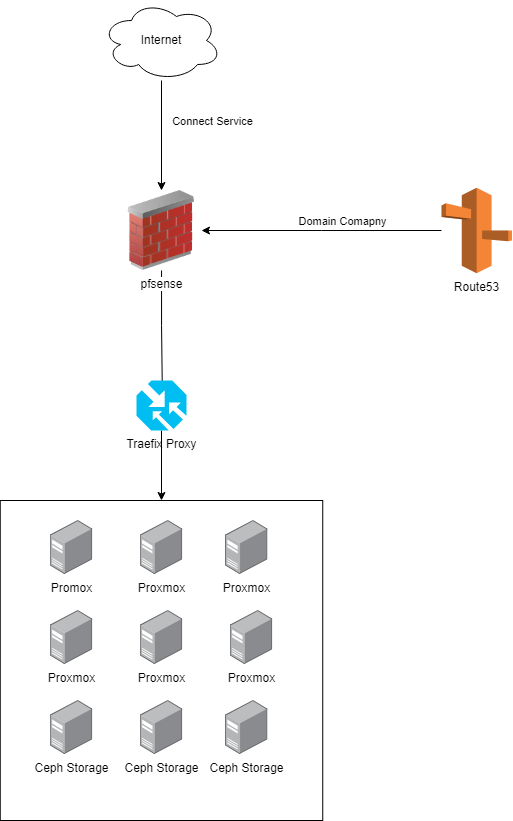
\includegraphics[width=0.7\linewidth]{Pics/diagram}
	\caption{\label{fig:diagram} Mô hình triển khai.}
	\label{fig:diagram}
	\end{figure}
	\section{Các bước triển khai Consul trên Kubernetes}
	\hspace{1.0cm}{Để triển khai Consul trên Kubernetes, chúng ta sẽ cần phải có những công cụ sau đây:\\}
	\begin{itemize}
		\item kubectl
		\item helm
		\item k9s
	\end{itemize}
	\hspace{0.3cm}{Dưới đây là các câu lệnh để triển khai Consul, chúng ta sẽ sử dụng Chart của Hashicorp cung cấp. Đầu tiên, chúng ta cần phải thêm nguồn chart vào trong dữ liệu Helm của chúng ta với câu lệnh sau:}
	\begin{lstlisting}[language=Bash]
	helm repo add hashicorp https://helm.releases.hashicorp.com
	\end{lstlisting}
	\hspace{1.0cm}{Tiếp theo, chúng ta sẽ cập nhật chart với câu lệnh: }
	\begin{lstlisting}[language=Bash]
	helm repo update
	\end{lstlisting}
	\hspace{1.0cm}{Sau đó, chúng ta tạo một tệp tin có tên là values.yaml, nội dung trong tệp tin như sau: }
	\begin{lstlisting}[language=Bash]
	global:
		name: consul
		datacenter: dc1
	server:
		replicas: 1
		storage: 10Gi
		storageClass: hostpath
	connectInject:
		enabled: true
	ui:
		enabled: true
	controller:
		enabled: true
	\end{lstlisting}
	\hspace{1.0cm}{Sau đó, chúng ta bắt đầu chạy câu lệnh sau:}
	\begin{lstlisting}[language=Bash]
	$ helm install -n consul consul -f consul/helm/consul/values.yaml hashicorp/consul
	NAME: consul
	LAST DEPLOYED: Tue Dec 20 20:12:02 2022   
	NAMESPACE: consul
	STATUS: deployed
	REVISION: 1
	NOTES:
	Thank you for installing HashiCorp Consul!
	
	Your release is named consul.
	
	To learn more about the release, run:     
	
	$ helm status consul --namespace consul 
	$ helm get all consul --namespace consul
	
	Consul on Kubernetes Documentation:       
	https://www.consul.io/docs/platform/k8s   
	
	Consul on Kubernetes CLI Reference:       
	https://www.consul.io/docs/k8s/k8s-cli
	\end{lstlisting}
	\hspace{1.0cm}{Vậy là chúng ta đã triển khai thành công Consul lên trên Kubernetes. Tiếp theo, chúng ta sẽ đến với các phần thực nghiệm.}
	\section{Thực nghiệm}
	\subsection{Kịch bản một: Mã hoá và thiết lập luật đường truyền giữa các micorserivce trong kubernetes}
	\subsubsection{Mô hình kịch bản}
	 \begin{figure}[h]
		\centering
		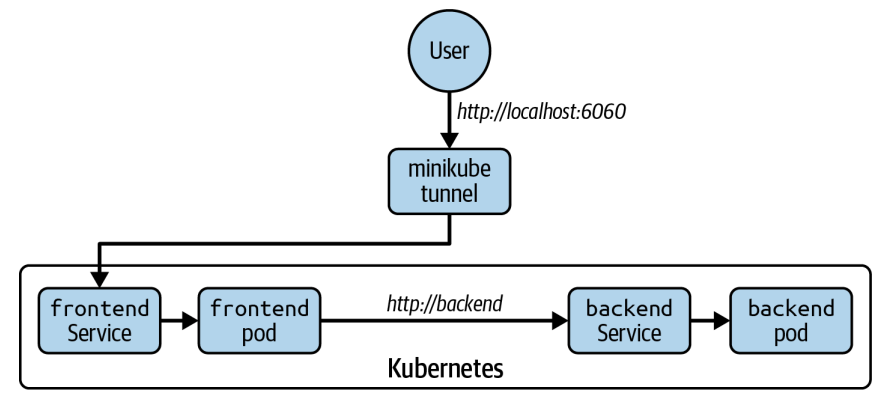
\includegraphics[width=1\linewidth]{Pics/kb1}
		\caption{\label{fig:kb1} Kịch bản một.}
		\label{fig:kb1}
	\end{figure}
	
	\hspace{1.0cm}{Ở trong kịch bản này, mục tiêu của chúng ta là sẽ tiến hành mã hoá và thiết lập các luật cho microservice. Các cách mã hoá sẽ được giải thích ở phần bên dưới.}
	\subsubsection{Thực nghiệm}
	\hspace{1.0cm}{Đầu tiên, chúng ta có tạo một tệp tin cấu hình của ứng dụng và service dành cho frontend, nội dung của tệp tin đó như sau:}
	\begin{lstlisting}[language=Bash]
		apiVersion: apps/v1
		kind: Deployment
		metadata:
			name: frontend
			labels:
				app: frontend
		spec:
			replicas: 1
			selector:
			matchLabels:
				app: frontend
			template:
				metadata:
					labels:
						app: frontend
				annotations:
					consul.hashicorp.com/connect-inject: 'true'
			spec:
				containers:
				  - name: frontend
				  image: ghcr.io/consul-up/birdwatcher-frontend:1.0.0
				  env:
					- name: BIND_ADDR
					  value: "0.0.0.0:6060"
					- name: BACKEND_URL
					  value: "http://backend"
				  ports:
				    - containerPort: 6060
	\end{lstlisting}

	\begin{lstlisting}[language=Bash]
		apiVersion: v1
		kind: Service
		metadata:
			name: frontend
				labels:
					app: frontend
		spec:
			type: LoadBalancer
			selector:
				app: frontend
			ports:
				- protocol: TCP
				  port: 6060
				  targetPort: 6060
	\end{lstlisting}
	\hspace{1.0cm}{Ở bên trên, lần lượt là nội dung của cấu hình dành cho ứng dụng frontend. Ứng dụng sẽ được triển khai theo kiểu deployment, tên của deployment là frontend và được gán label với key là app và value là frontend. Tiếp theo, số lượng pod được sao chép nhau được định nghĩa là 1, và bên số lượng bản sao sẽ có cùng một cấu hình được mô phỏng theo trường template ở bên dưới. Ứng dụng sẽ được thêm một trường annotation, trường này sẽ có tác dụng ghi đè cấu hình của Consul lên trên ứng dụng. Ở đây, chúng ta sẽ truyền vào annotaions là pod sẽ được inject sidecar đi kèm với ứng dụng. Cuối cùng, phần ứng dụng sẽ là một image có tên là \textit{ghcr.io/consul-up/birdwatcher-frontend:1.0.0}, các bản sao sẽ dựa trên image này và bắt đầu khởi chạy ứng dụng. Các biến môi trường được truyền vào theo kiểu khoá và giá trị, các giá trị này sẽ giúp cho ứng dụng chạy trên ip là 0.0.0.0 với cổng là 6060 và đường dẫn tới ứng dụng backend là \textit{http://backend}. Cổng của ứng dụng sẽ được mở là cổng 6060.}
	
	\hspace{0.3cm}{Với tệp cấu hình service, chúng ta sẽ tạo cho ứng dụng một service có tên là frontend, loại của service này là \textit{LoadBalancer}, giao thức của ứng dụng này được sử dụng là TCP, cổng của service là 6060 và cổng của container được service trỏ vào là 6060.}
	
	\hspace{0.3cm}{Tiếp theo đấy, là tệp tin cấu hình của ứng dụng và service dành cho  backend, tệp tin có nội dung như sau:}
		\begin{lstlisting}[language=Bash]
		apiVersion: apps/v1
		kind: Deployment
		metadata:
			name: backend
				labels:
					app: backend
		spec:
			replicas: 1
			selector:
				matchLabels:
					app: backend
			template:
				metadata:
					labels:
						app: backend
				annotations:
					consul.hashicorp.com/connect-inject: 'true'
				spec:
					containers:
					  - name: backend
				 	  image: ghcr.io/consul-up/birdwatcher-frontend:1.0.0
					  env:
						- name: BIND_ADDR
						  value: "0.0.0.0:7000"
					  ports:
					  	- containerPort: 7000
	\end{lstlisting}

	\begin{lstlisting}[language=Bash]
		apiVersion: v1
		kind: Service
		metadata:
			name: backend
				labels:
					app: backend
		spec:
			type: LoadBalancer
				selector:
					app: backend
			ports:
				- protocol: TCP
				  port: 80
				  targetPort: 7000
	\end{lstlisting}
	\hspace{1.0cm}{Tương tự như frontend, ứng dụng backend sẽ được cấu hình theo kiểu Deployment. Tên của deployment là backend và được gán label với key là app và value là backend. Tiếp theo, số lượng pod được sao chép nhau được định nghĩa là 1, và bên số lượng bản sao sẽ có cùng một cấu hình được mô phỏng theo trường template ở bên dưới. Ứng dụng sẽ được thêm một trường annotation, trường này sẽ có tác dụng ghi đè cấu hình của Consul lên trên ứng dụng. Ở đây, chúng ta sẽ truyền vào annotaions là pod sẽ được inject sidecar đi kèm với ứng dụng. Cuối cùng, phần ứng dụng sẽ là một image có tên là \textit{ghcr.io/consul-up/birdwatcher-backend:1.0.0}, các bản sao sẽ dựa trên image này và bắt đầu khởi chạy ứng dụng. Các biến môi trường được truyền vào theo kiểu khoá và giá trị, các giá trị này sẽ giúp cho ứng dụng chạy trên ip là 0.0.0.0 với cổng là 7000. Cổng của ứng dụng sẽ được mở là cổng 7000.}

	\hspace{0.3cm}{Với tệp cấu hình service, chúng ta sẽ tạo cho ứng dụng một service có tên là backend, loại của service này không được định nghĩa, nên kubernetes sẽ tự ngầm hiểu là kiểu \textit{ClusterIP}, giao thức của ứng dụng này được sử dụng là TCP, cổng của service là 80 và cổng của container được service trỏ vào là 7000.}
	
	\hspace{0.3cm}{Sau khi chúng ta có sao chép nội dung vào các tệp tin, chúng ta sẽ di chuyển chúng vào trong một thư mục. Ở đây, chúng ta sẽ di chuyển vào thư mục \textit{/c/Users/justo/Desktop/Helm-chart/nestjs-helm/consul/manifest/application}. Để chạy các ứng dụng, chúng ta sẽ bắt sử dụng câu lệnh sau:}
	\begin{lstlisting}[language=Bash]
	kubectl apply -f /c/Users/justo/Desktop/Helm-chart/nestjs-helm/consul/manifest/application/. 
	\end{lstlisting}

	\hspace{1.0cm}{Sau khi apply, ứng dụng sẽ được triển khai trên sẽ mất một thời gian để ở trạng thái ready. Để kiểm tra trạng thái ứng dụng, chúng ta sẽ chạy lệnh sau:}
	\begin{lstlisting}[language=Bash]
	$ kubectl get deployment,service --selector app=frontend
	NAME                       READY   UP-TO-DATE   AVAILABLE   AGE
	deployment.apps/frontend   1/1     1            1           2d20h
	
	NAME               TYPE           CLUSTER-IP      EXTERNAL-IP   PORT(S)          AGE
	service/frontend   LoadBalancer   10.110.206.79   localhost     6060:32589/TCP   2d20h
	\end{lstlisting}
	\begin{lstlisting}[language=Bash]
	$ k get deployment,service --selector app=backend
	NAME                      READY   UP-TO-DATE   AVAILABLE   AGE
	deployment.apps/backend   1/1     1            1           2d20h
	
	NAME              TYPE        CLUSTER-IP     EXTERNAL-IP   PORT(S)   AGE
	service/backend   ClusterIP   10.103.28.18   <none>        80/TCP    2d20h
	\end{lstlisting}

	\hspace{0.3cm}{Ở đây, con số của trạng thái sẵn sàng là 1/1, thì ứng dụng của chúng ta đã được triển khai thành công. Service của các ứng dụng đã được mở cổng như chúng ta mong đợi. Và tiếp theo, chúng ta sẽ bắt đầu truy cập vào UI của ứng dụng frontend và xem kết quả.}
	
	\hspace{0.3cm}{Để truy cập được vào UI của ứng dụng, chúng ta sẽ sử dụng câu lệnh port-forward để mở port của ứng dụng ra bên ngoài máy của chúng ta. Câu lệnh được thực thi như sau:}
	\begin{lstlisting}[language=Bash]
	kubectl port-forward service/frontend 6060
	\end{lstlisting}
	\hspace{1.0cm}{Sau khi port-forward thành công, chúng ta mở trình duyệt web lên và tiến hành truy cập vào địa chỉ \textit{http://localhost:6060} để kiểm tra kết quả.}
	\pagebreak
	
	\begin{figure}[h]
		\centering
		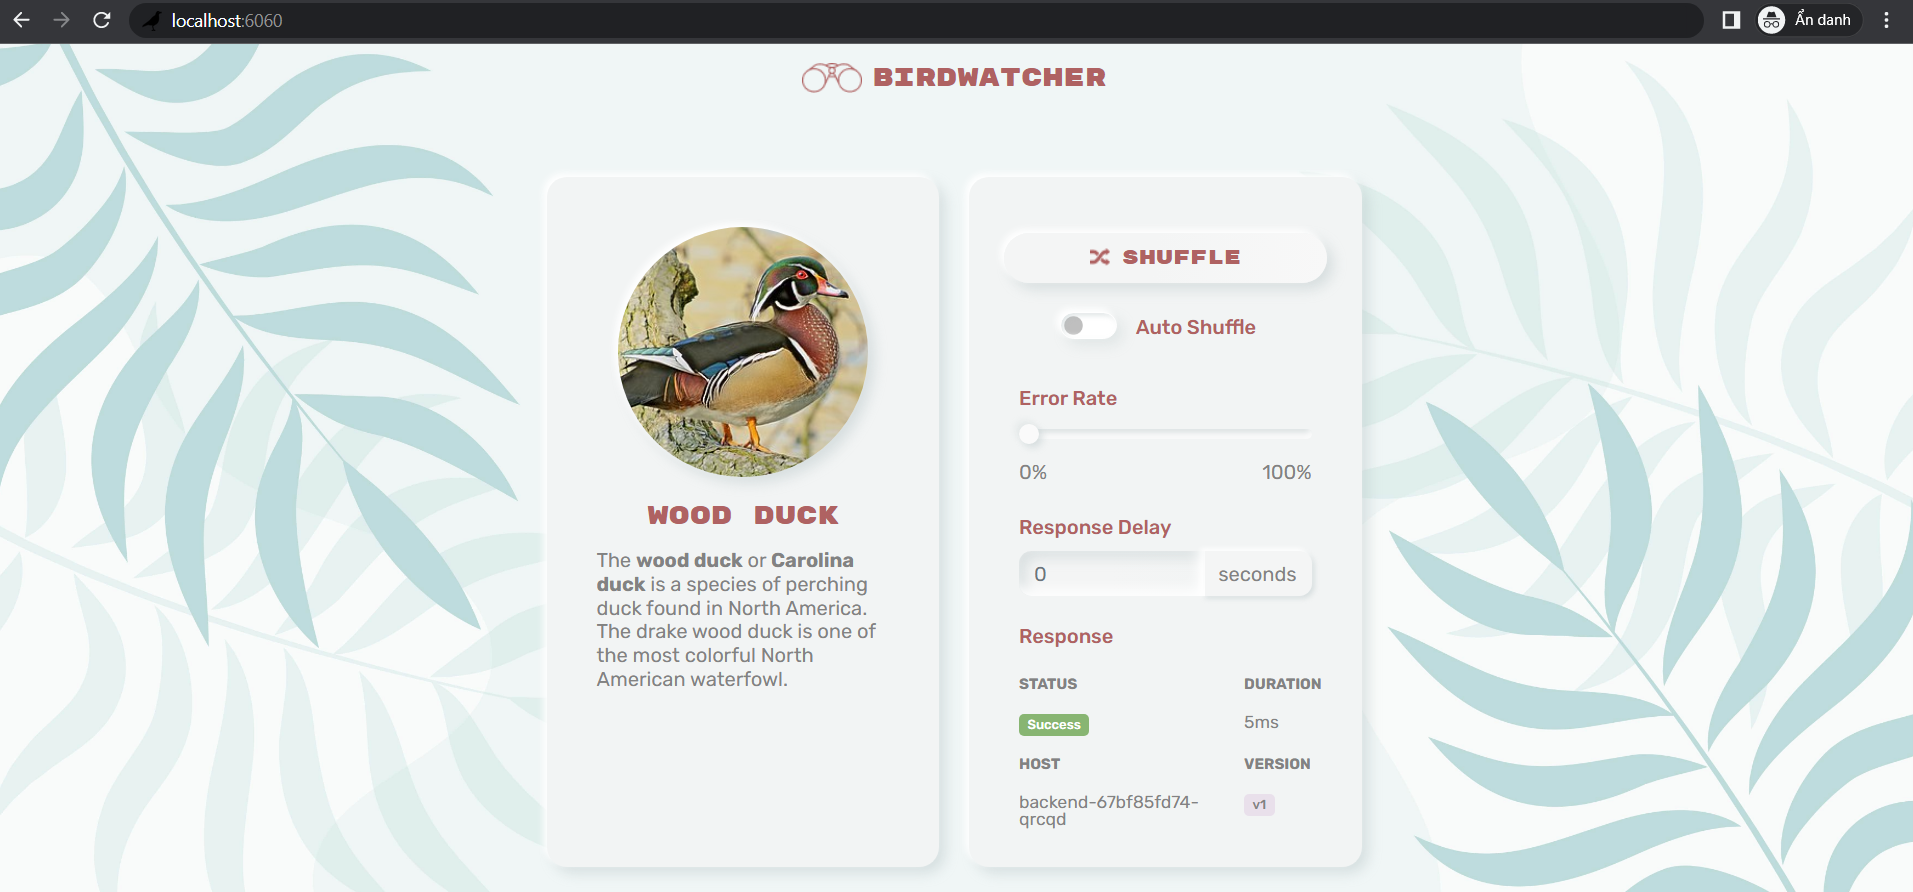
\includegraphics[width=1\linewidth]{Pics/localhost-6060}
		\caption{\label{fig:localhost-6060} Giao diện ứng dụng frontend.}
		\label{fig:localhost-6060}
	\end{figure}

	\hspace{0.3cm}{Tiếp theo, chúng ta đã thêm annotations vào trong tệp cấu hình, chúng ta sẽ port-forward tiếp consul server tương tự như trên và chúng ta tiến hành vào giao diện của consul với địa chỉ \textit{http://localhost:8500} để xem kết quả mà chúng ta đã truyền sidecar đi kèm với ứng dụng.}
	
	\begin{figure}[h]
		\centering
		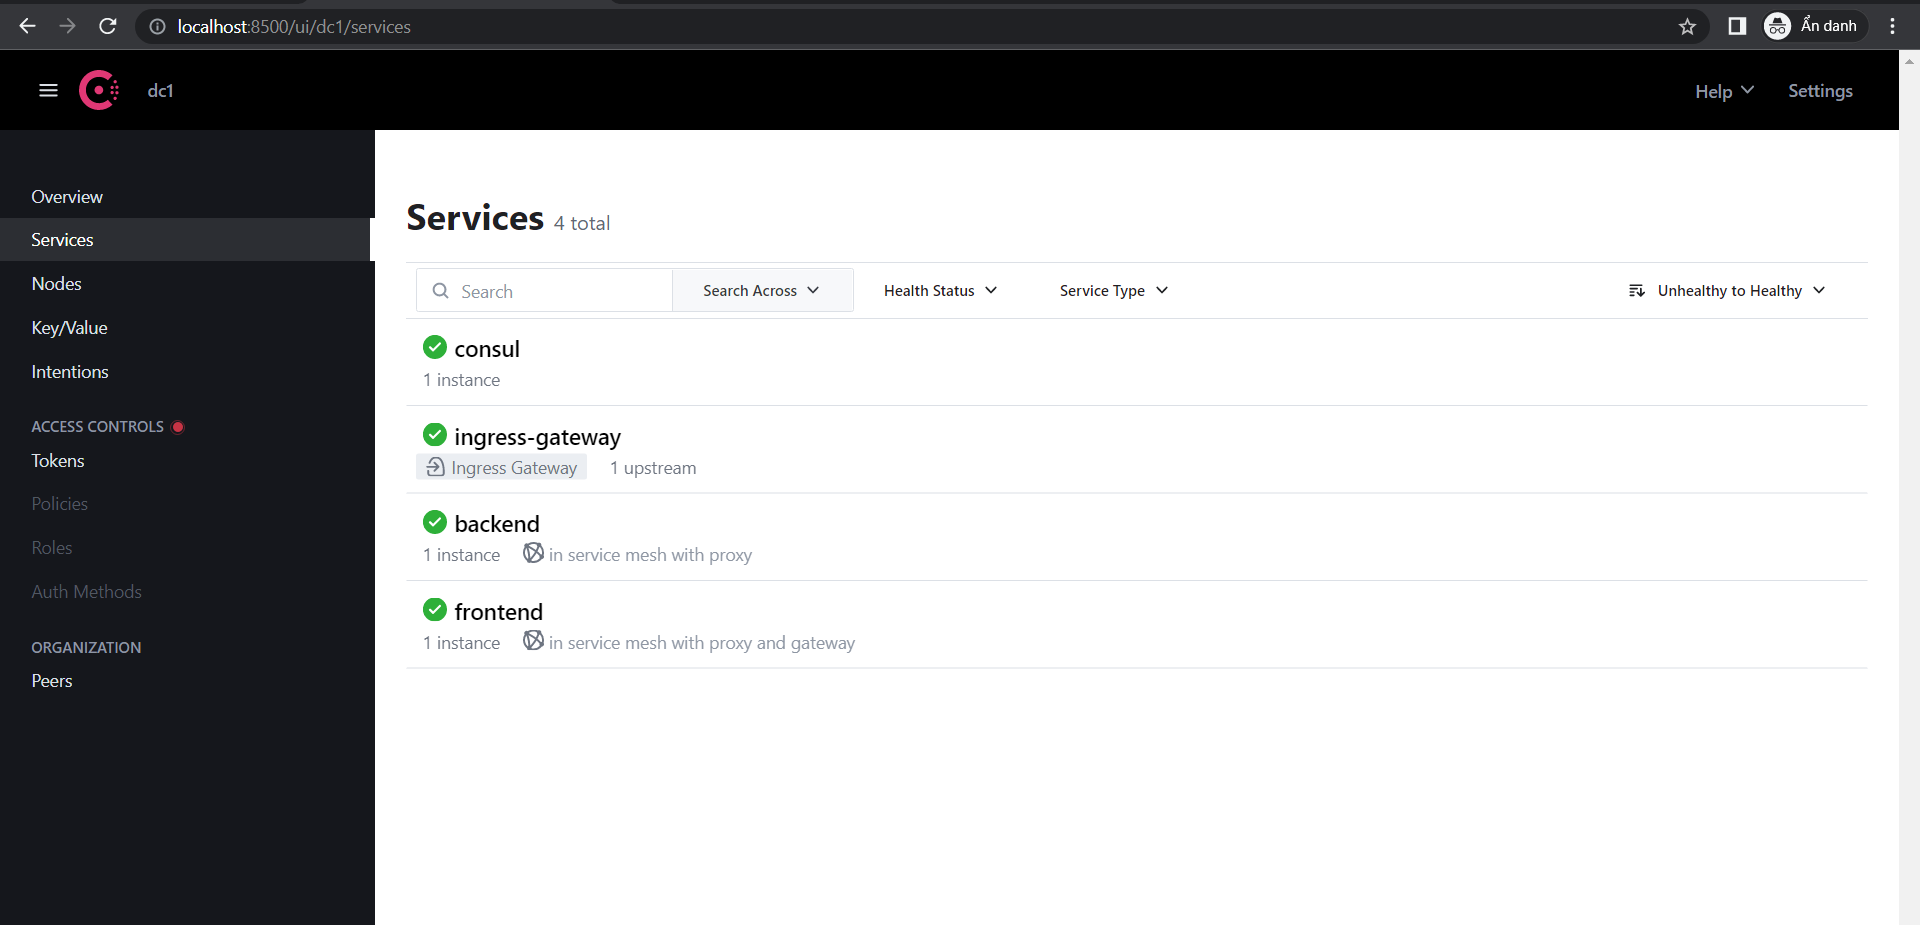
\includegraphics[width=1\linewidth]{Pics/localhost-8500}
		\caption{\label{fig:localhost-8500} Giao diện Consul Server.}
		\label{fig:localhost-8500}
	\end{figure}
	\hspace{0.3cm}{Như vậy, chúng ta đã thành công truyền proxy đi kèm với ứng dụng frontend và backend, hay nói cách khác, ứng dụng frontend và backend đang là một phần của service mesh. Sau đấy, chúng ta sẽ quay lại trang web \textit{http://localhost:6060} lúc nãy, tải lại trang và kiểm tra kết quả. Nếu như trang trả lại lỗi như bên dưới, thì mọi thứ vẫn đang đúng như những gì chúng ta đã làm.}
	\pagebreak
	\begin{figure}[h]
		\centering
		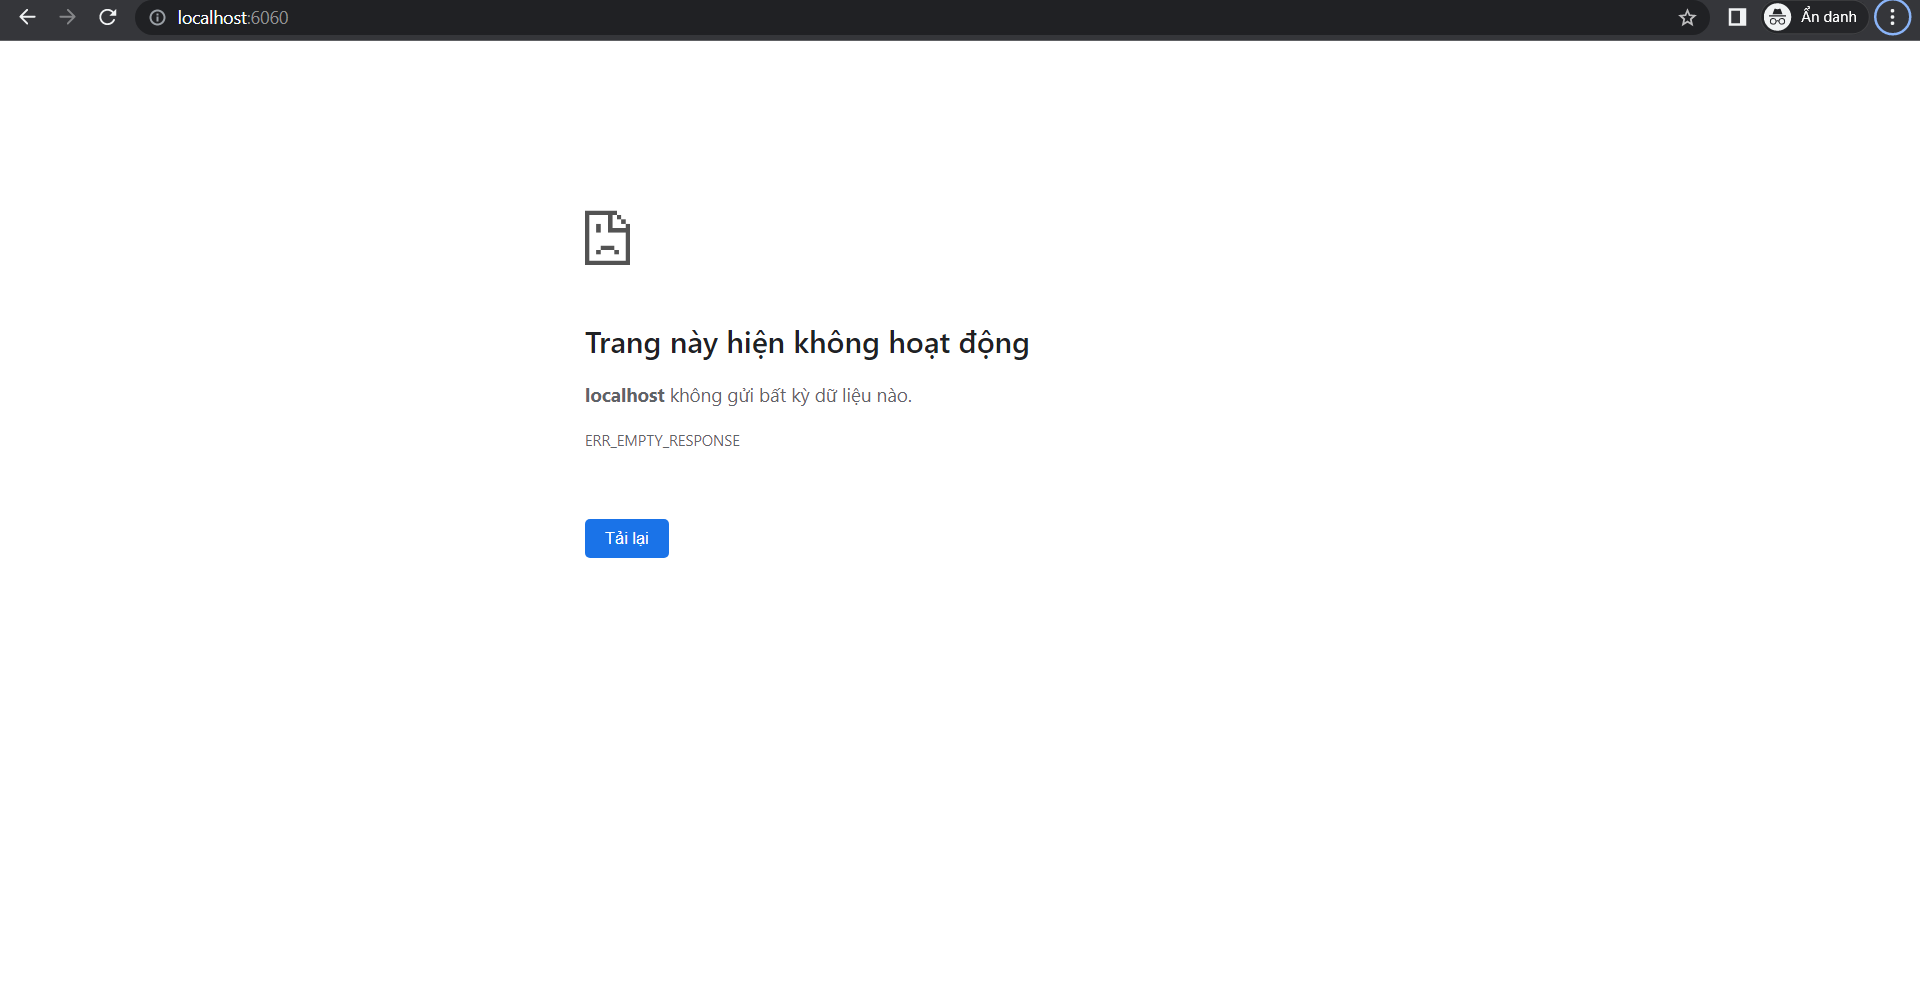
\includegraphics[width=1\linewidth]{Pics/localhost-6060-error}
		\caption{\label{fig:localhost-6060-error} Lỗi khi vào tải lại trang.}
		\label{fig:localhost-6060-error}
	\end{figure}

	\hspace{0.3cm}{Lý do mà trang không thể tải lại được, nguyên nhân là do ứng dụng frontend đang là một phần của service mesh. Sidecar proxy đã chặn tất cả các nguồn đi vào được trong ứng dụng. Consul đã bảo mật ứng dụng và yêu cầu tất cả các luồng đi vào service mesh cần phải được xác thực và uỷ quyền.  Khi mà chúng ta request tới frontend, thì chúng ta chưa xác thực và nhận được quyền truy cập vào trong frontend nên Consul đã từ chối và không cho phép chúng ta truy cập. Nếu như chúng ta truy cập được bằng port-forward, thì portforward đã cho phép chúng ta bỏ qua luật của consul và truy cập thẳng vào trong ứng dụng frontend.}
	
	\hspace{0.3cm}{Ở trên giao diện của Consul, chúng ta click vào các service, ở đây, giao diện sẽ hiện ra các cấu trúc giữa các service mesh với nhau.}
	
	\begin{figure}[h]
		\centering
		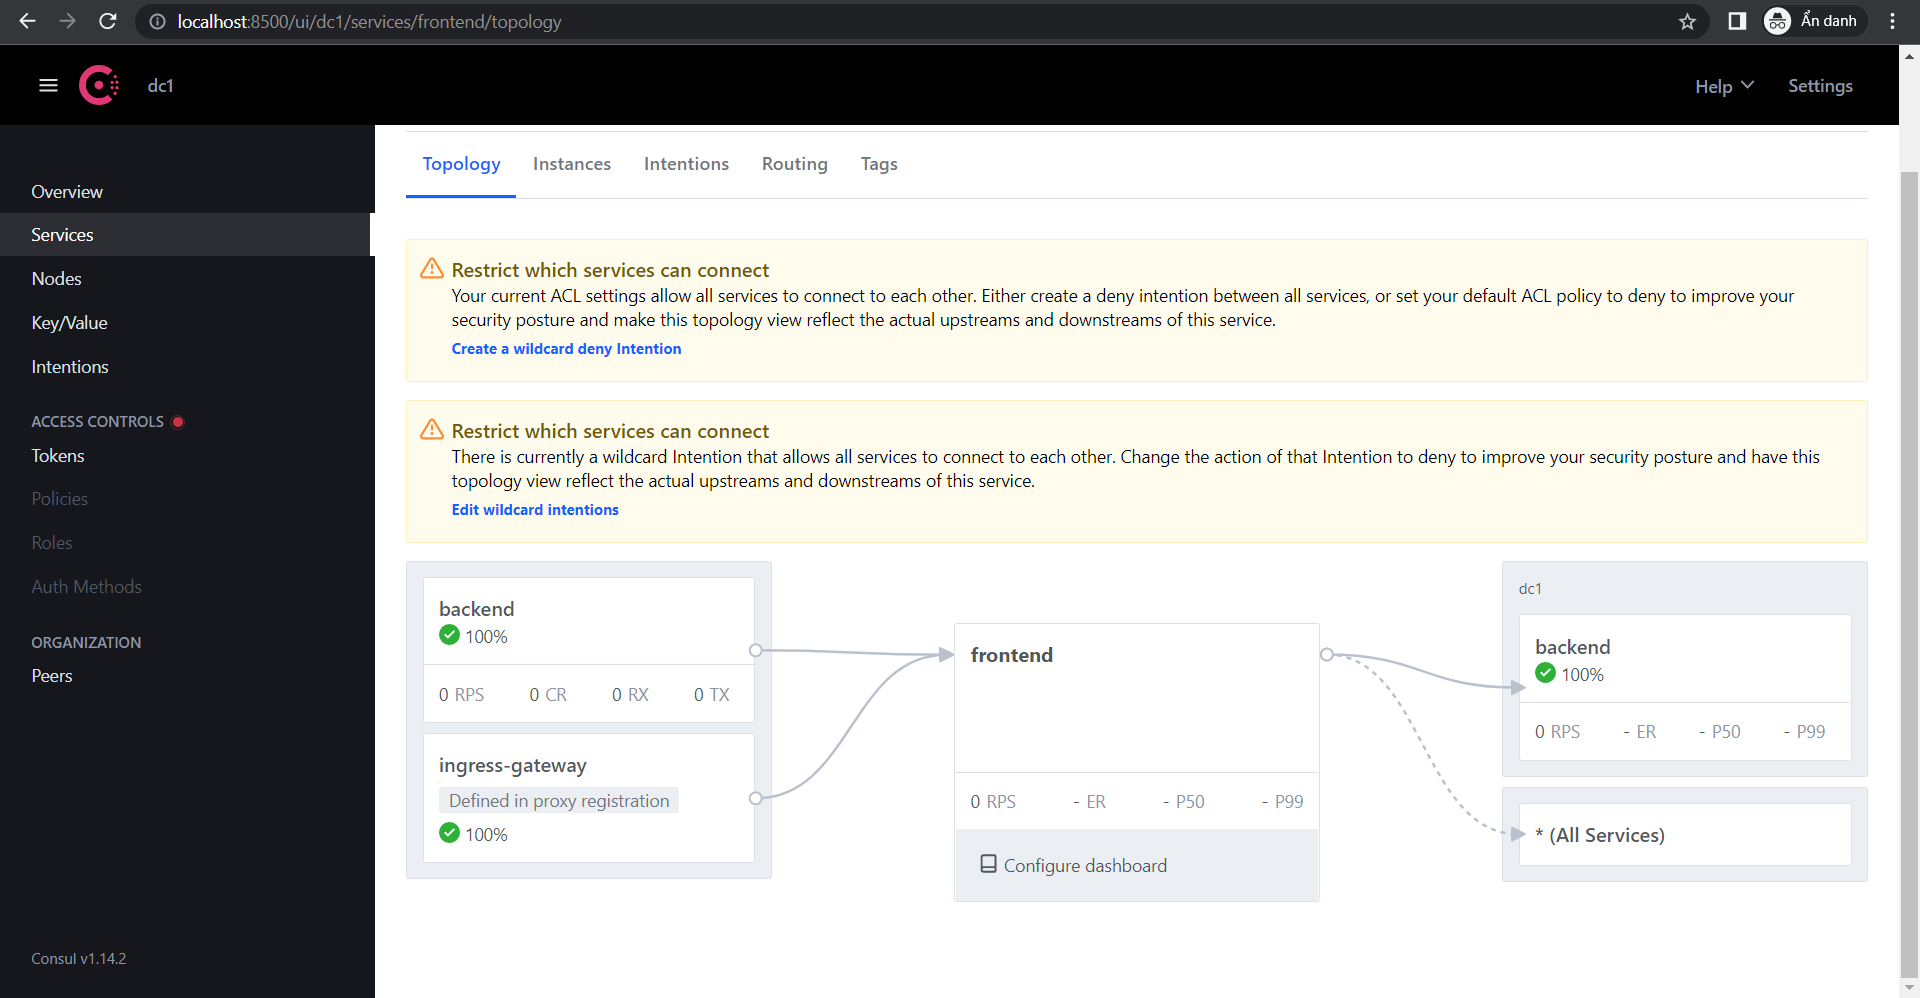
\includegraphics[width=1\linewidth]{Pics/topology}
		\caption{\label{fig:topology} Cấu trúc của service frontend.}
		\label{fig:topology}
	\end{figure}
	
	\hspace{0.3cm}{Tiếp theo, chúng ta sẽ tiến hành thiết lập luật dành cho service frontend và backend. Để thiết lập, chúng ta có 2 cách để làm, cách thứ nhất là chúng ta có thể làm trực tiếp trên giao diện, nhưng mà chúng ta không nên sử dụng cách này, vì sau khi chúng ta di dời Consul sang một bên khác, thì chúng ta sẽ lại phải thiết lập bằng tay tất cả các service. Việc này khá là tốn effort dành cho người quản trị. Với cách thứ hai, chúng ta có thể viết cấu hình vào một tiệp loại yaml dành cho kubernetes. Tệp cấu hình có nội dung như sau:}
	\begin{lstlisting}[language=Bash]
		apiVersion: consul.hashicorp.com/v1alpha1
		kind: ServiceIntentions
		metadata:
			name: frontend
			namespace: consul
		spec:
			destination:
			  name: frontend
			sources:
			- name: backend
			  action: allow
	\end{lstlisting}
	\hspace{1.0cm}{Sau khi tạo một tệp với nội dung bên trên, chúng ta tiến hành apply nó và lên trên giao diện của Consul Server và xem kết quả.}
	
	\begin{figure}[h]
		\centering
		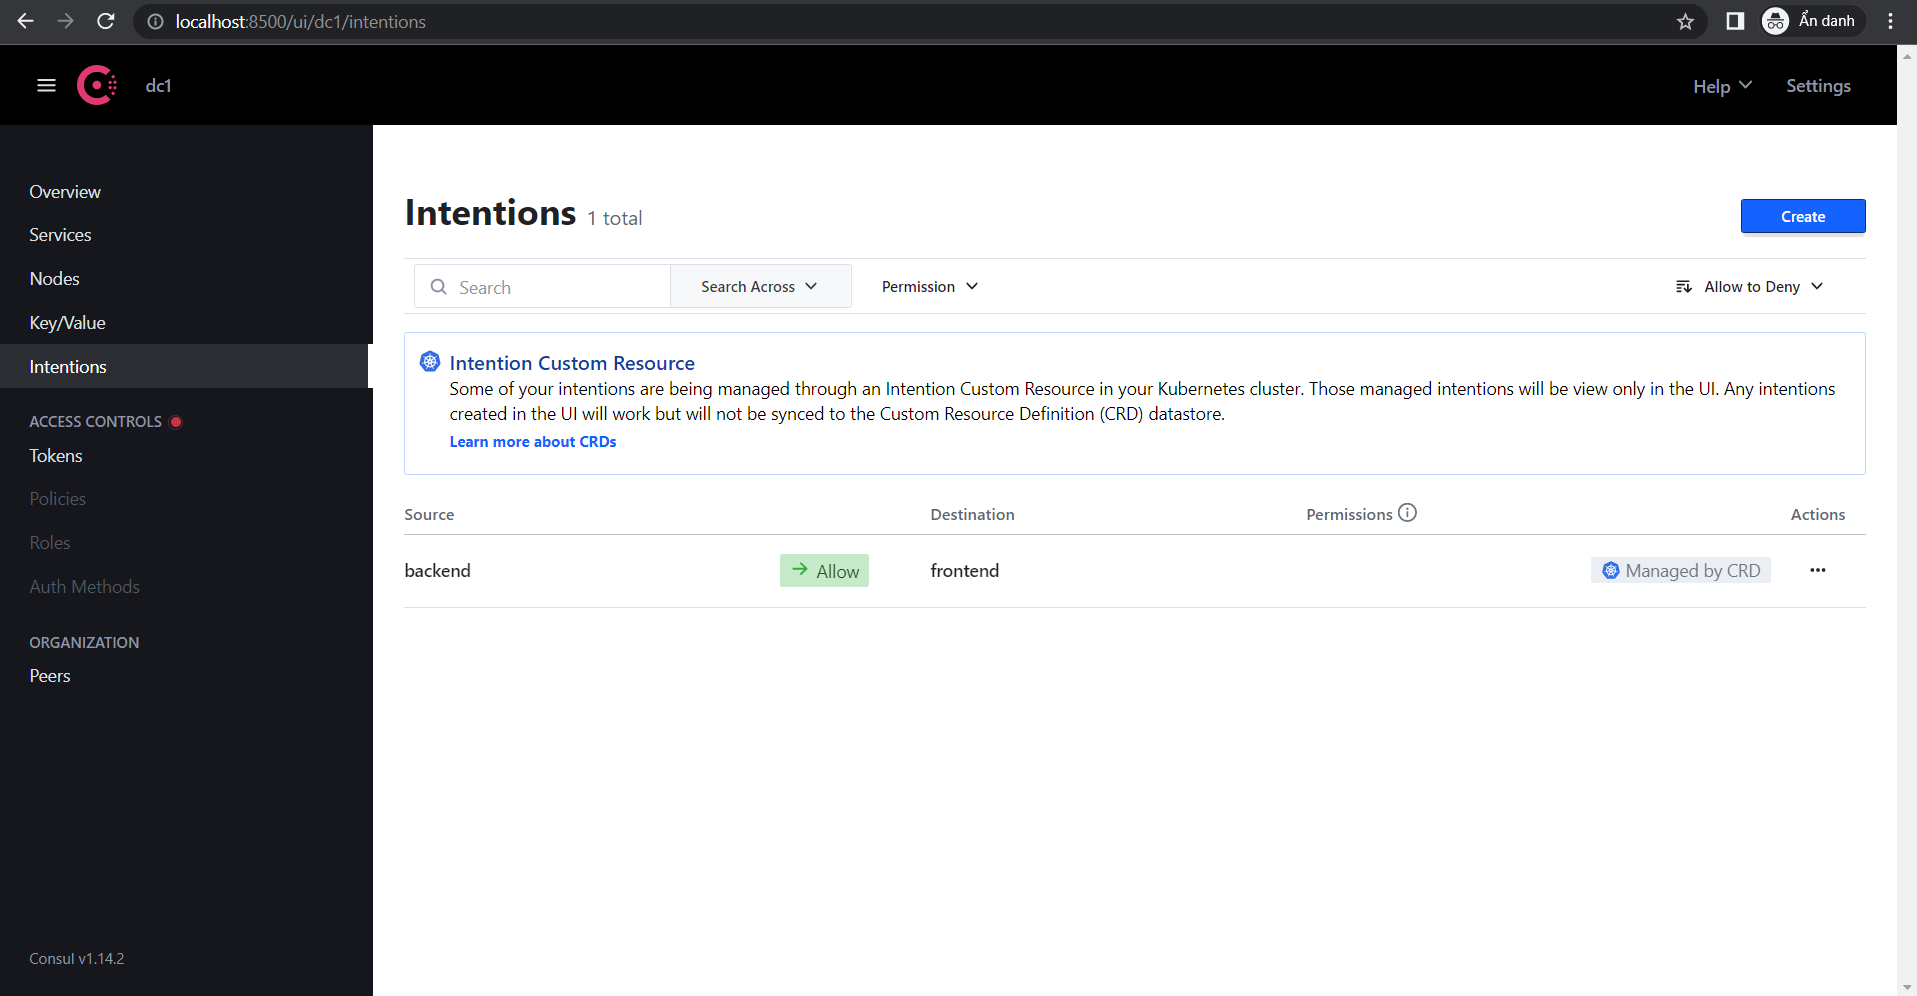
\includegraphics[width=1\linewidth]{Pics/intention-1}
		\caption{\label{fig:intention-1} Intention sau khi được cấu hình.}
		\label{fig:intention-1}
	\end{figure}

	\hspace{0.3cm}{Với luật này, chúng ta cho phép service backend được kết nối tới service frontend. Tuy nhiên, đến đây vẫn chưa xong, vì mặc định của proxy là giao tiếp thông qua giao thức tcp, mà ứng dụng frontend và backend giao tiếp thông qua giao thức http. Vì vậy, chúng ta cần cài đặt lại để cho proxy nhận truy cập http. Để cấu hình, chúng ta cần tạo 1 tệp tin với nội dung như sau:}
	\begin{lstlisting}[language=Bash]
	apiVersion: consul.hashicorp.com/v1alpha1
	kind: ProxyDefaults
	metadata:
		name: global
		namespace: consul
	spec:
		config:
		protocol: http
	\end{lstlisting}
	\hspace{1.0cm}{Sau khi cấu hình xong, chạy lệnh sau để kiểm tra:}
	\begin{lstlisting}[language=Bash]
	$ kubectl get proxydefaults.consul.hashicorp.com  -A
	NAMESPACE   NAME     SYNCED   LAST SYNCED   AGE
	consul      global   True     90m           90m
	\end{lstlisting}
	\hspace{1.0cm}{Như vậy, với status là synced, thì có nghĩa là ứng dụng đã có thể giao tiếp với nhau thông qua giao thức http.}
	
	\hspace{0.3cm}{Tiếp theo đấy, chúng ta sẽ kiểm tra xem thông tin chứng chỉ mà Consul tạo ra cho ứng dụng. Để kiểm tra, đầu tiên chúng ta cần truy cập được vào trong container ứng dụng với câu lệnh sau:}
	\begin{lstlisting}[language=Bash]
		kubectl exec deploy/backend -c backend -- \
		sh -c 'openssl s_client -connect $(hostname -i):20000 | \
		openssl x509 -noout -text'
		--------------------------------------------
		openssl x509 -noout -text'
		Can't use SSL_get_servername
		depth=0
		verify error:num=20:unable to get local issuer certificate
		verify return:1
		depth=0
		verify error:num=21:unable to verify the first certificate
		verify return:1
		depth=0
		verify return:1
		DONE
		Certificate:
		Data:
		Version: 3 (0x2)
		Serial Number: 39 (0x27)
		Signature Algorithm: ecdsa-with-SHA256
		Issuer: CN = pri-1r5tjaui.consul.ca.562ec48b.consul
		Validity
		Not Before: Dec 20 13:12:29 2022 GMT
		Not After : Dec 23 13:12:29 2022 GMT
		Subject:
		Subject Public Key Info:
		Public Key Algorithm: id-ecPublicKey
		Public-Key: (256 bit)
		pub:
		04:1c:cd:db:7b:49:00:e2:9a:48:97:71:31:88:32:
		45:85:c8:15:01:82:b9:27:34:eb:0b:a0:63:02:7d:
		fe:1e:af:a2:42:e8:26:1f:19:43:2a:51:d5:bf:46:
		42:0f:f5:65:36:29:2d:05:ff:80:d4:23:93:49:00:
		18:1f:44:1f:dd
		ASN1 OID: prime256v1
		NIST CURVE: P-256
		X509v3 extensions:
		X509v3 Key Usage: critical
		Digital Signature, Key Encipherment, Data Encipherment, Key Agreement
		X509v3 Extended Key Usage:
		TLS Web Client Authentication, TLS Web Server Authentication
		X509v3 Basic Constraints: critical
		CA:FALSE
		X509v3 Subject Key Identifier:
		BB:38:30:7C:86:88:A3:DC:AB:43:69:77:6B:B9:43:95:81:D1:25:47:E4:FA:9C:D6:AB:C2:A1:FE:99:51:FA:F7
		X509v3 Authority Key Identifier:
		keyid:0B:A1:BC:23:3F:15:0E:84:6B:32:30:E2:03:42:68:1B:2B:99:FF:7F:78:F1:71:0B:9D:70:5A:C0:F0:DE:66:A0
		
		X509v3 Subject Alternative Name: critical
		URI:spiffe://562ec48b-2872-87db-c307-d5435d3d833e.consul/ns/default/dc/dc1/svc/backend
		Signature Algorithm: ecdsa-with-SHA256
		30:45:02:21:00:ed:64:a1:78:0e:09:8b:fc:6c:ea:10:76:5b:
		57:c5:a3:c5:8c:0d:b2:ab:65:12:a1:67:45:0f:31:7d:dc:fd:
		74:02:20:15:ab:1c:60:c6:64:91:2e:0f:0b:bb:47:33:a2:24:
		13:54:3d:0a:fe:3b:8f:c6:e7:53:ea:e2:47:c6:65:75:79
	\end{lstlisting}
	\hspace{1.0cm}{Đây là chứng chỉ mà Consul tạo ra để mã hoá các dữ liệu được truyền qua nhau thông qua proxy. Các chứng chỉ này được tạo ra bởi Consul, ở đây Consul đóng vai trò là một cơ quan cấp chứng chỉ và cấp cho mỗi Service. Dưới đây là cách mà Consul tạo ra chứng chỉ để mã hoá và dùng chứng chỉ để giải mã dữ liệu.}
	\pagebreak
	\begin{figure}[h]
		\centering
		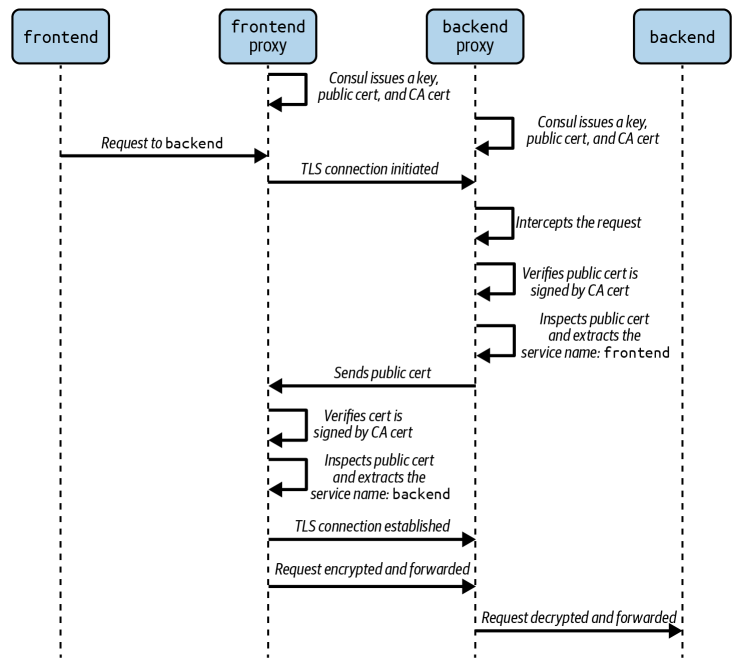
\includegraphics[width=1\linewidth]{Pics/certificate}
		\caption{\label{fig:certificate} Biểu đồ tuần tự trong giao tiếp của ứng dụng frontend và backend.}
		\label{fig:certificate}
	\end{figure}

	\hspace{0.3cm}{Với mỗi chứng chỉ, Consul sẽ mã hoá ID của mỗi service được gọi là SPIFFE ID, mỗi ID được gắn vào chứng chỉ và chỉ có Consul có thể giải mã được được ID đấy. Cho nên, nếu như hacker có thể xâm nhập được vào ứng dụng, nhưng khi gọi các service, hacker sẽ không có được ID để mã hoá và gửi cho các service kia.}
	\subsubsection{Đánh giá}
	\hspace{1.0cm}{Qua kịch bản trên, chúng ta đã có thể mã hoá giao tiếp giữa các service với nhau thông qua TLS cũng như thiết lập các luật giao tiếp của chúng với nhau. Tuy nhiên, khi mà chúng ta thiết lập xong như vậy, thì làm thế nào để chúng ta không cần xác thực và được uỷ quyền đến từ consul mà vẫn có thể truy cập được ứng dụng, chúng ta sẽ đến kịch bản 2, triển khai Ingress Gateway cho các service.}
	\subsection{Kịch bản hai: Triển khai ingress gateway cho các service}
	\subsubsection{Mô tả kịch bản}
	\pagebreak
	\begin{figure}[h]
		\centering
		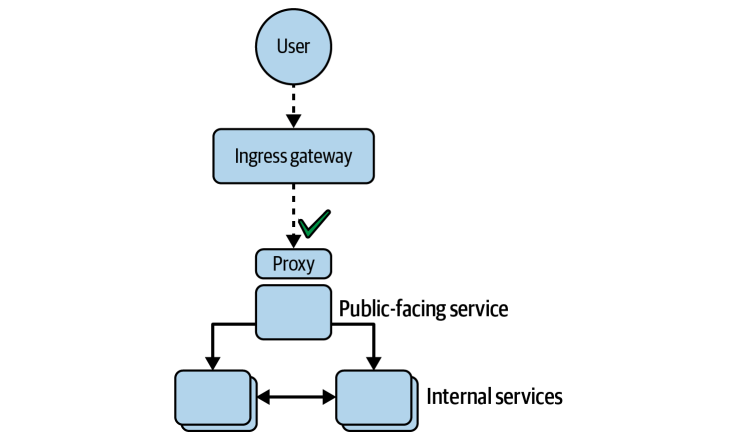
\includegraphics[width=1\linewidth]{Pics/ingress-gateway}
		\caption{\label{fig:ingress-gateway} Luồng truy cập của người dùng vào trong ứng dụng thông qua ingress-gateway.}
		\label{fig:ingress-gateway}
	\end{figure}
	
	\hspace{1.0cm}{Để giúp cho người dùng có thể truy cập được ứng dụng mà không cần sự đồng ý của Consul, thì chúng ta sẽ tiến hành tạo ra một trong những thành phần của Consul là ingress gateway. Ingress gateway ở đây sẽ đóng một vai trò là sẽ điều hướng toàn bộ yêu cầu vào và chuyển các yêu cầu đấy tới các service tương ứng. Vậy làm thế nào để tạo ra ingress gateway, làm sao để có thể điều hướng vào các dịch vụ tương ứng, chúng ta sẽ đến với phần thực nghiệm.}
	
	\subsubsection{Thực nghiệm}
	\hspace{1.0cm}{Đầu tiên, để tạo ra ingress gateway, thì chúng ta cần cập nhật tệp tin values.yaml ở phần các bước triển khai. Chúng ta sẽ thêm vào một phần sau vào bên dưới tệp:}
	\begin{lstlisting}[language=Bash]
	ingressGateways:
		enabled: true
		defaults:
			replicas: 1	
			service:
				type: LoadBalancer
	\end{lstlisting}
	\hspace{1.0cm}{Sau khi thêm vào, chúng ta sẽ chạy câu lệnh sau để update chart của Consul}
	\begin{lstlisting}[language=Bash]
	helm upgrade -n consul consul -f /c/Users/justo/Desktop/Helm-chart/nestjs-helm/consul/helm/values.yaml hashicorp/consul
	\end{lstlisting}
	\hspace{1.0cm}{Sau khi helm upgrade xong chart, thì chúng ta sẽ truy cập vào giao diện của Consul và xem kết quả:}
	\pagebreak
	\begin{figure}[h]
	\centering
	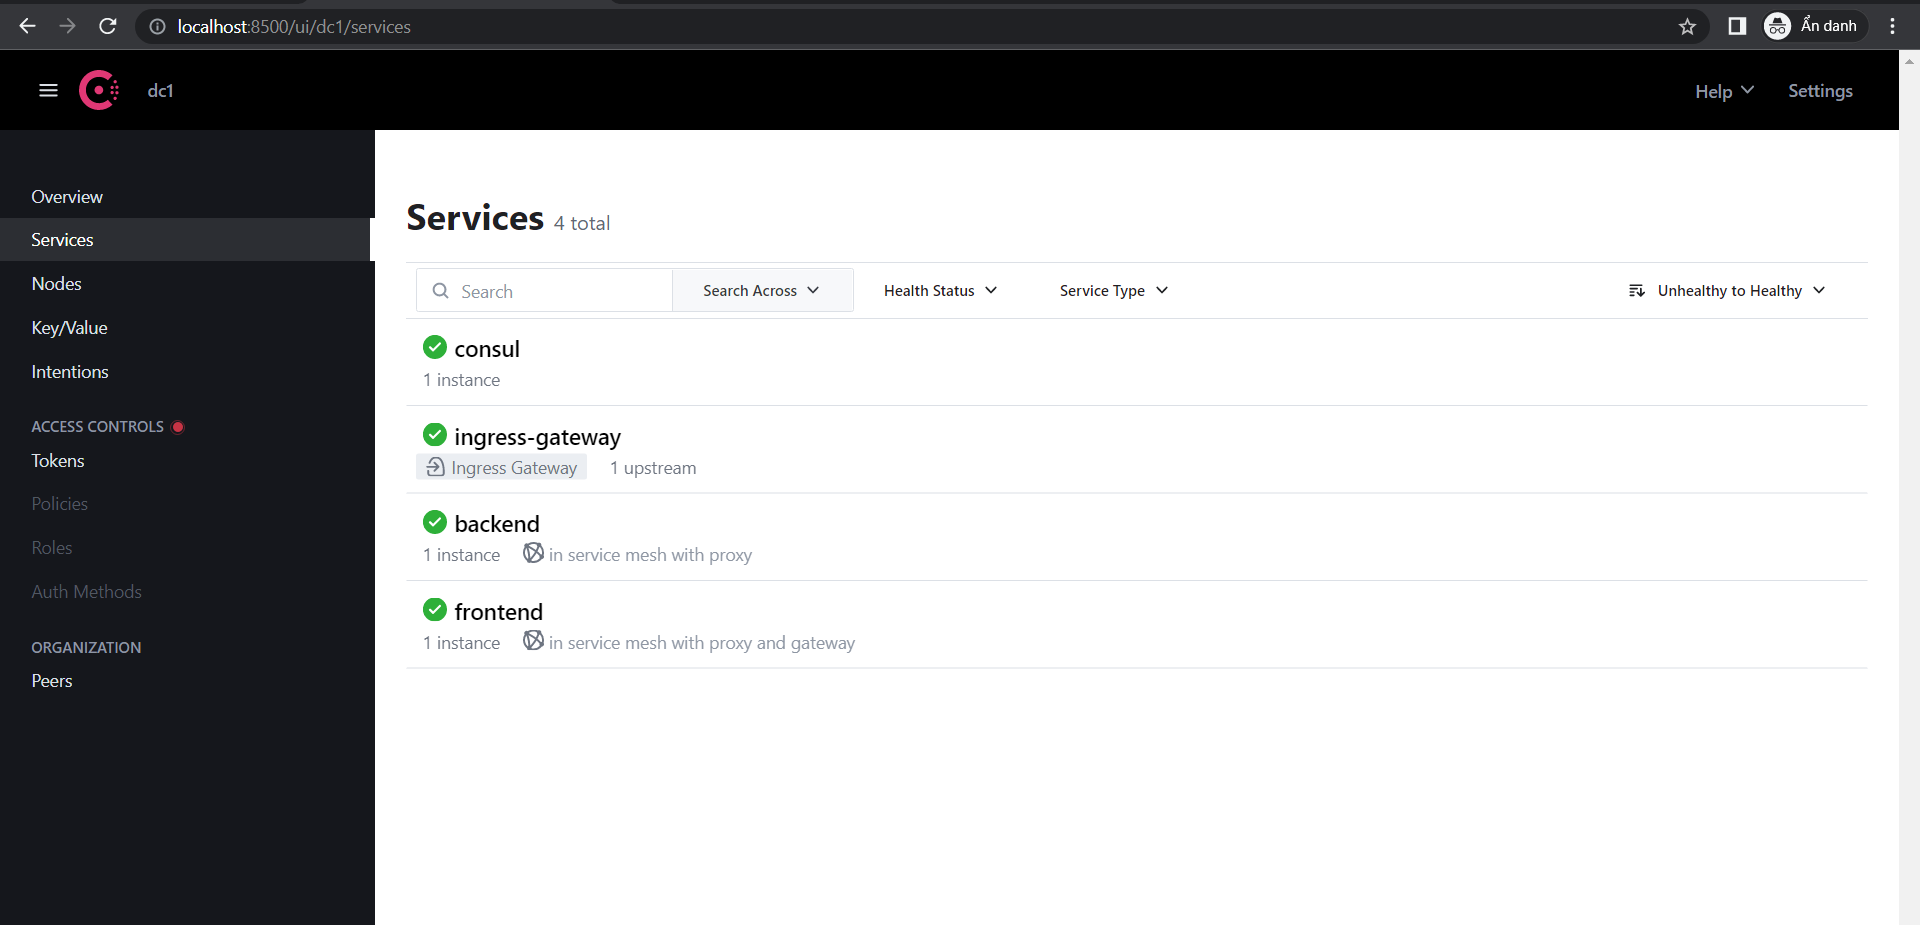
\includegraphics[width=1\linewidth]{Pics/localhost-8500}
	\caption{\label{fig:localhost-8500} Ingress Gateway đã hiện bên trên giao diện.}
	\label{fig:localhost-8500}
	\end{figure}

	\hspace{0.3cm}{Tiếp theo, chúng ta tiến tới cấu hình điều hướng cho người dùng có thể truy cập vào ứng dụng thông qua ingress gateway. Để làm được, chúng ta sẽ có một tệp tin cấu hình của ingress gateway, nội dung của tệp tin như sau:}
	\begin{lstlisting}[language=Bash]
		apiVersion: consul.hashicorp.com/v1alpha1
		kind: IngressGateway
		metadata:
			name: ingress-gateway
			namespace: consul
		spec:
			listeners:
				- port: 8080
				  protocol: http
				  services:
					- name: frontend
					  hosts: ["localhost"]
	\end{lstlisting}
	\hspace{1.0cm}{Khi chúng ta có tệp tin, bắt đầu chạy lệnh để apply nội dung và lên trên UI của Consul để kiểm tra. Để vào xem thông tin, chúng ta vào Service -> Ingress-Gateway -> Upstream và kiểm tra:}
	 \begin{figure}[h]
		\centering
		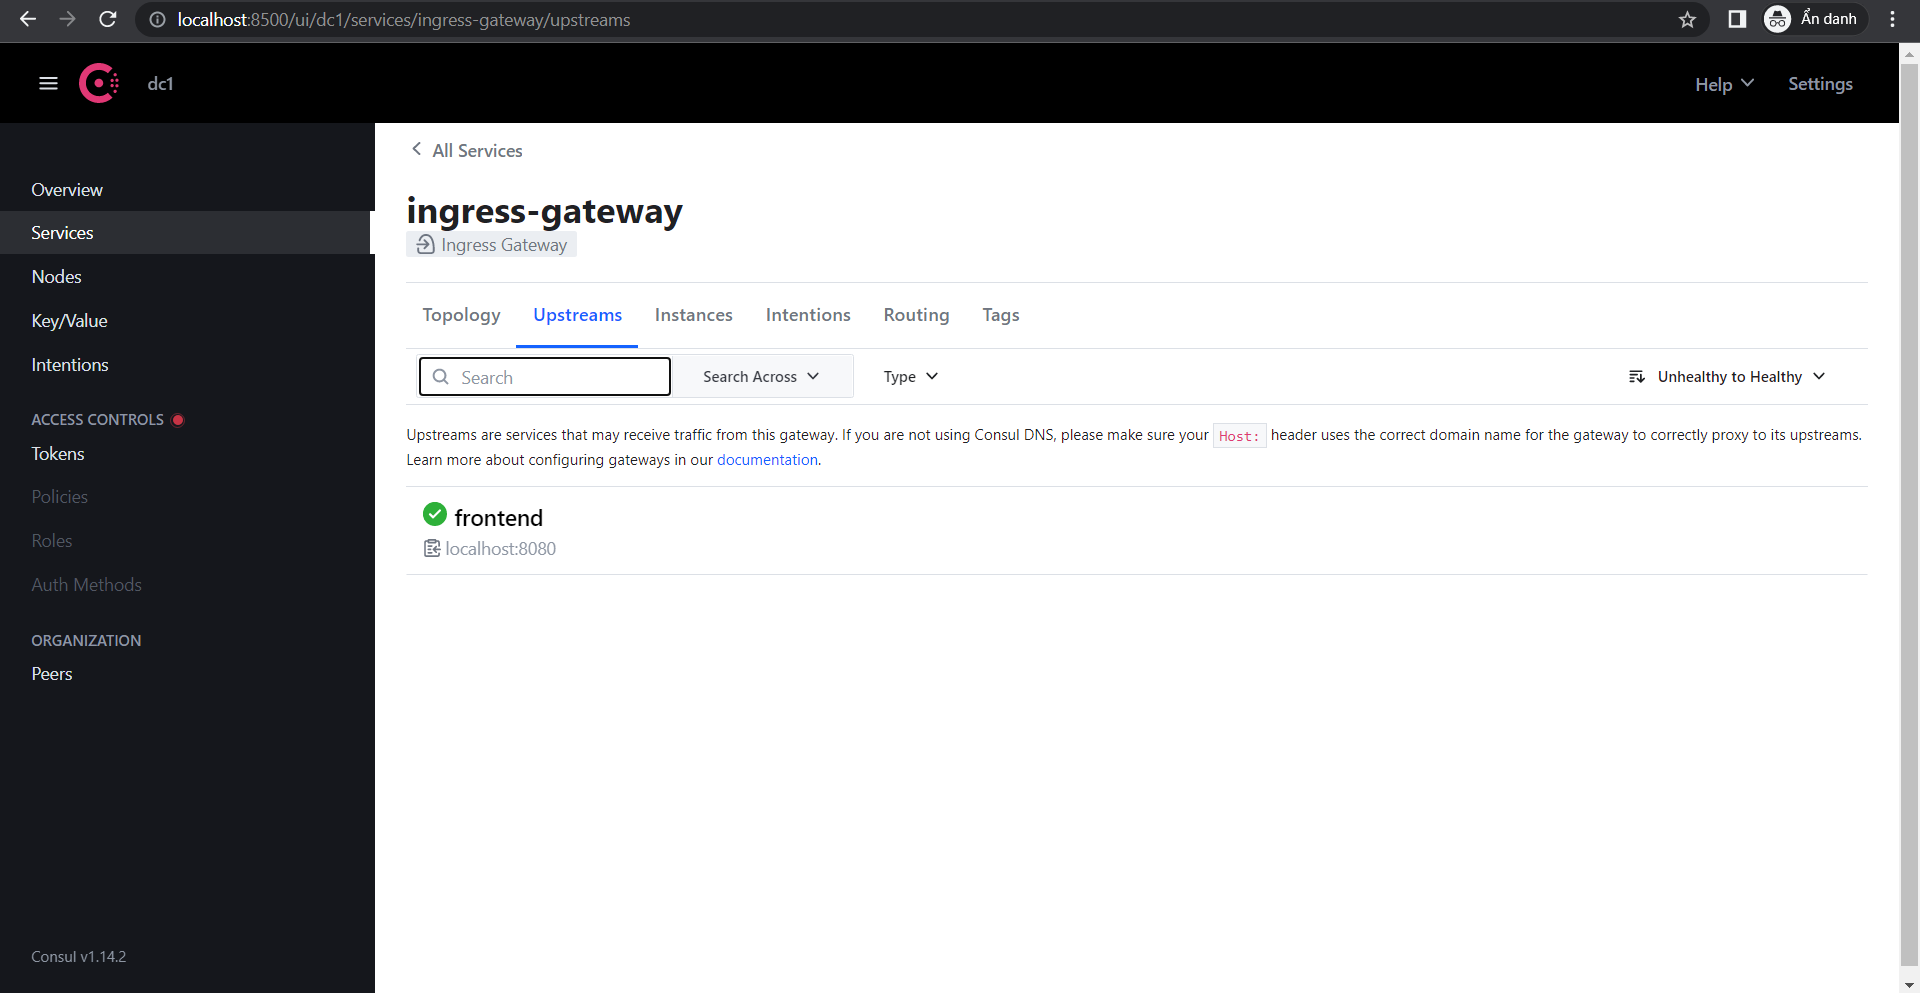
\includegraphics[width=1\linewidth]{Pics/upstream}
		\caption{\label{fig:upstream} Cấu hình điều hướng truy cập tới ứng dụng frontend.}
		\label{fig:upstream}
	\end{figure}
	\hspace{0.3cm}{Như vậy, ứng dụng đã có thể truy cập thông qua ingress gateway. Để truy cập, chúng ta truy cập vào địa chỉ \textit{http://localhost:8080} để kiểm tra.}
	 \begin{figure}[h]
		\centering
		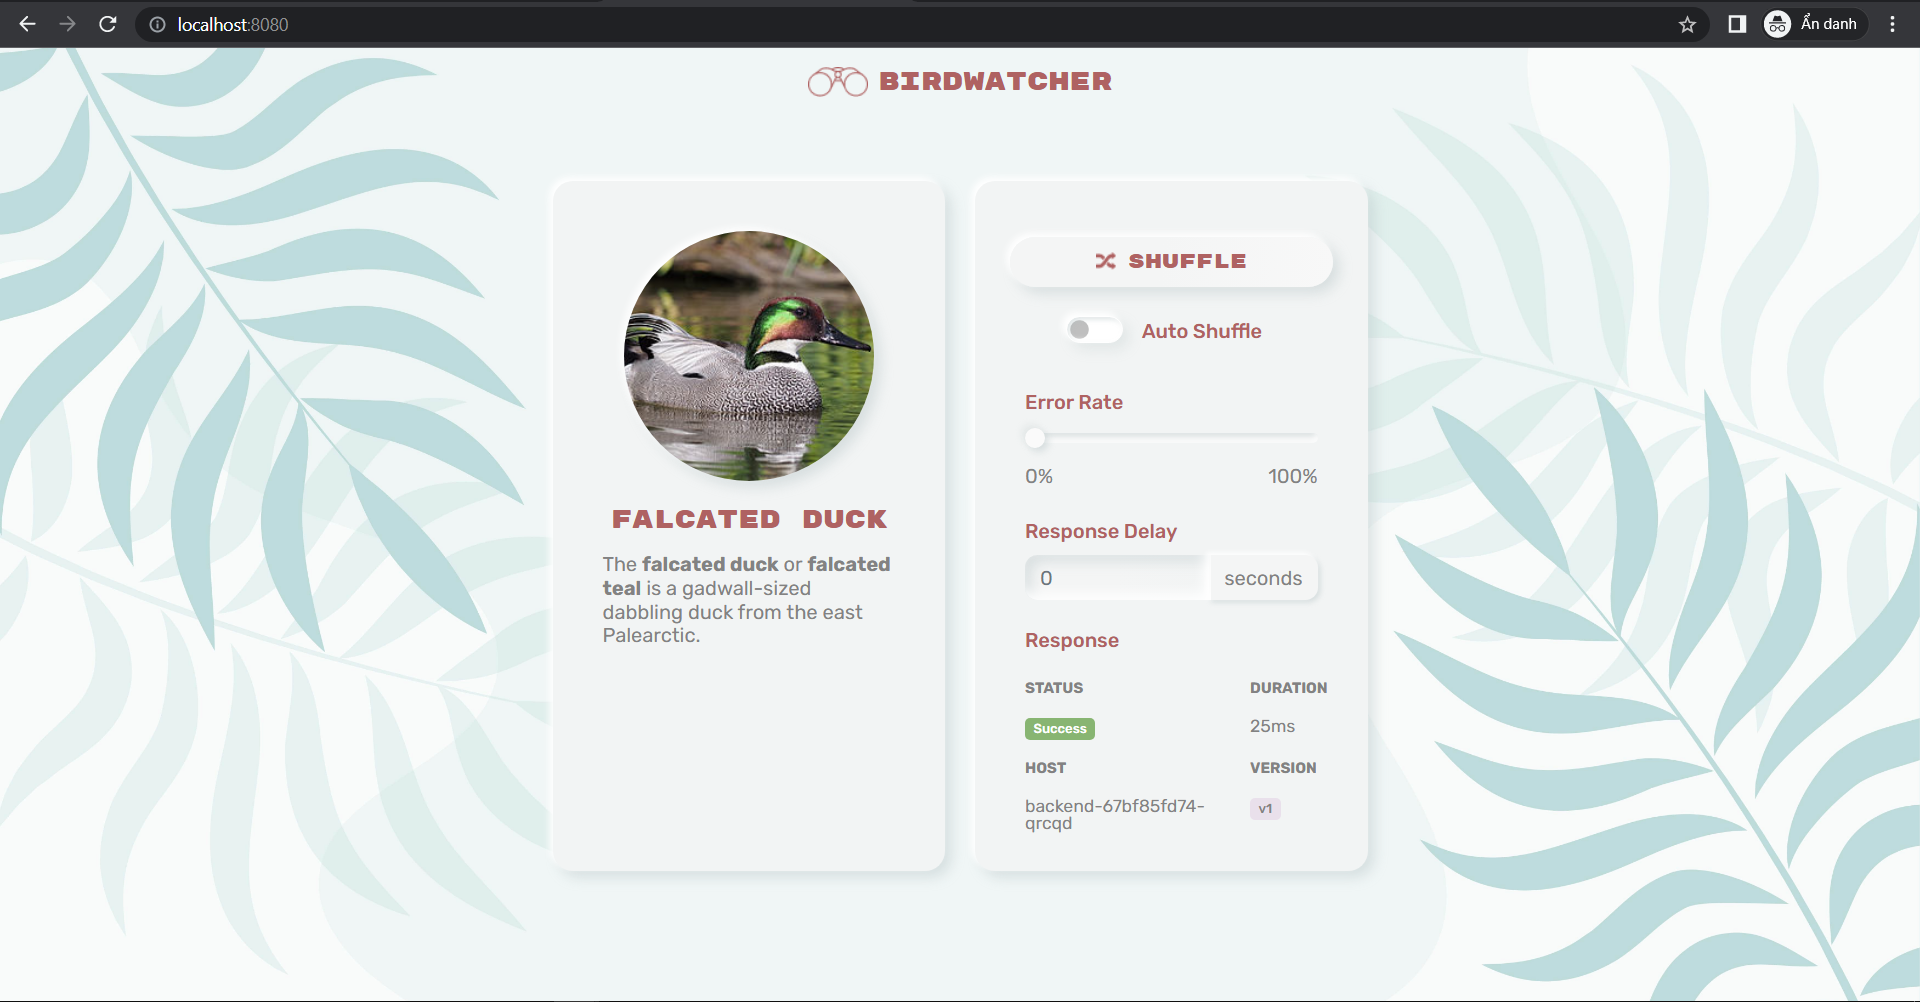
\includegraphics[width=1\linewidth]{Pics/localhost-8080}
		\caption{\label{fig:localhost-8080} Dịch vụ frontend khi được mở thông qua ingress gateway.}
		\label{fig:localhost-8080}
	\end{figure}
	\hspace{0.3cm}{Như vậy chúng ta đã cấu hình thành công để công khai dịch vụ ra ngoài thông qua ingress gateway.}
	\subsubsection{Đánh giá}
	\hspace{1.0cm}{Thông qua triển khai trên, chúng ta đã tiến hành tạo ra ingess gateway để công khai dịch vụ ra ngoài mà không cần phải được quyền cho phép của Consul. Tiếp theo, chúng ta sẽ đến phần điều tra. Khi mà ứng dụng của chúng ta có vấn đề, thì chúng ta cần phải điều tra những nguyên nhân gây ra vấn đề đó. Đó có thể là do Ingress gateway không hoạt động, hay các luật cấu hình sai. Để biết được, chúng ta đến phần tiếp theo, điều tra nguyên nhân gián đoạn của dịch vụ}
	\subsection{Kịch bản ba: Điều tra nguyên nhân gián đoạn dịch vụ}
	\subsubsection{Mô tả kịch bản}
	\begin{figure}[h]
	\centering
	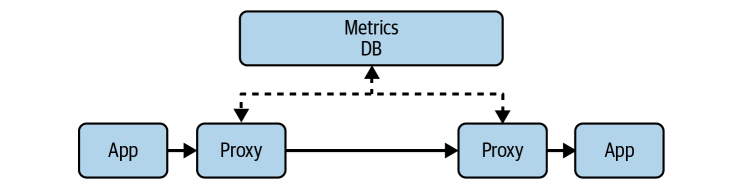
\includegraphics[width=1\linewidth]{Pics/metrics}
	\caption{\label{fig:metrics} Đẩy metrics của proxy lên một Metrics DB.}
	\label{fig:metrics}
	\end{figure}
	\hspace{1.0cm}{Ở phần này, chúng ta sẽ tiến hành đẩy các metrics của proxy lên một nơi có thể đọc được các thông số Metrics. Ở đây, chúng ta sẽ sử dụng Prometheus. Prometheus là một phần đi kèm luôn với chart của Consul. Nếu như chúng ta đã sử dụng Prometheus đã có sẵn, thì chúng ta sẽ không cần phải thêm vào chart và sẽ cấu hình Promtheus có sẵn để thu thập các metrics được đẩy ra bởi proxy. Ở phần thực nghiệm này, chúng ta sẽ sử dụng Prometheus của chart Consul để tiến hành thu thập dữ liệu.}
	\subsubsection{Thực nghiệm}
	\hspace{1.0cm}{Trước khi bắt đầu, chúng ta cần phải triển khai prometheus để thu thập dữ liệu. Để có prometheus, chúng ta sẽ cập nhật lại chart như sau:}
	\begin{lstlisting}[language=Bash]
	prometheus:
		enabled: true
	\end{lstlisting}
	\hspace{1.0cm}{Tiếp đó, chúng ta bắt đầu cấu hình proxy để proxy có thể đẩy các metrics ra bên ngoài. Để cấu hình, tệp values.yaml chúng ta cần chỉnh sửa lại như sau:}
	\begin{lstlisting}[language=Bash]
	connectInject:
		enabled: true
		default: false
		metrics:
			defaultEnabled: true
			defaultEnableMerging: true
			defaultPrometheusScrapePort: 20200
			defaultPrometheusScrapePath: "/metrics"
			defaultMergedMetricsPort: 20100
	\end{lstlisting}
	\hspace{1.0cm}{Với cấu hình trên, chúng ta đã cấu hình đẩy các metrics ra bên ngoài với cổng 20220 và với path là /metrics. Prometheus của Consul sử dụng đã có cấu hình sẵn để thu thập dữ liệu từ cổng và đường dẫn kia nên chúng ta sẽ không cần phải cấu hình lại Prometheus. }
	\hspace{0.3cm}{Tiếp theo, chúng ta sẽ cấu hình để hiển thị thông tin metrics trên UI của Consul. Để làm vậy, chúng ta tiếp tục cập nhật nội dung của tệp values.yaml thành như sau:}
	\begin{lstlisting}[language=Bash]
	ui:
		enabled: true
		service:
			type: NodePort
		metrics:
			provider: "prometheus"
			baseURL: http://prometheus-server
	\end{lstlisting}
	\hspace{1.0cm}{Cấu hình trên, do Promtheus được triển khai ở cùng với namespace Consul, nên chúng ta chỉ cần khai báo tên service của Promtheus là được. Sau đó, chúng ta tiến hành nâng cấp chart để chart nhận config mới với câu lệnh sau:}
	\begin{lstlisting}[language=Bash]
		helm upgrade -n consul consul -f /c/Users/justo/Desktop/Helm-chart/nestjs-helm/consul/helm/values.yaml hashicorp/consul
	\end{lstlisting}
	\hspace{1.0cm}{Vậy là chúng ta đã xong phần triển khai Prometheus cũng như tiến hành đẩy các metrics từ proxy lên Prometheus. Để kiểm tra, chúng ta sẽ port-forward service của Prometheus để kiểm tra trên đường dẫn \textit{http://localhost:9090}.}
	\begin{figure}[h]
		\centering
		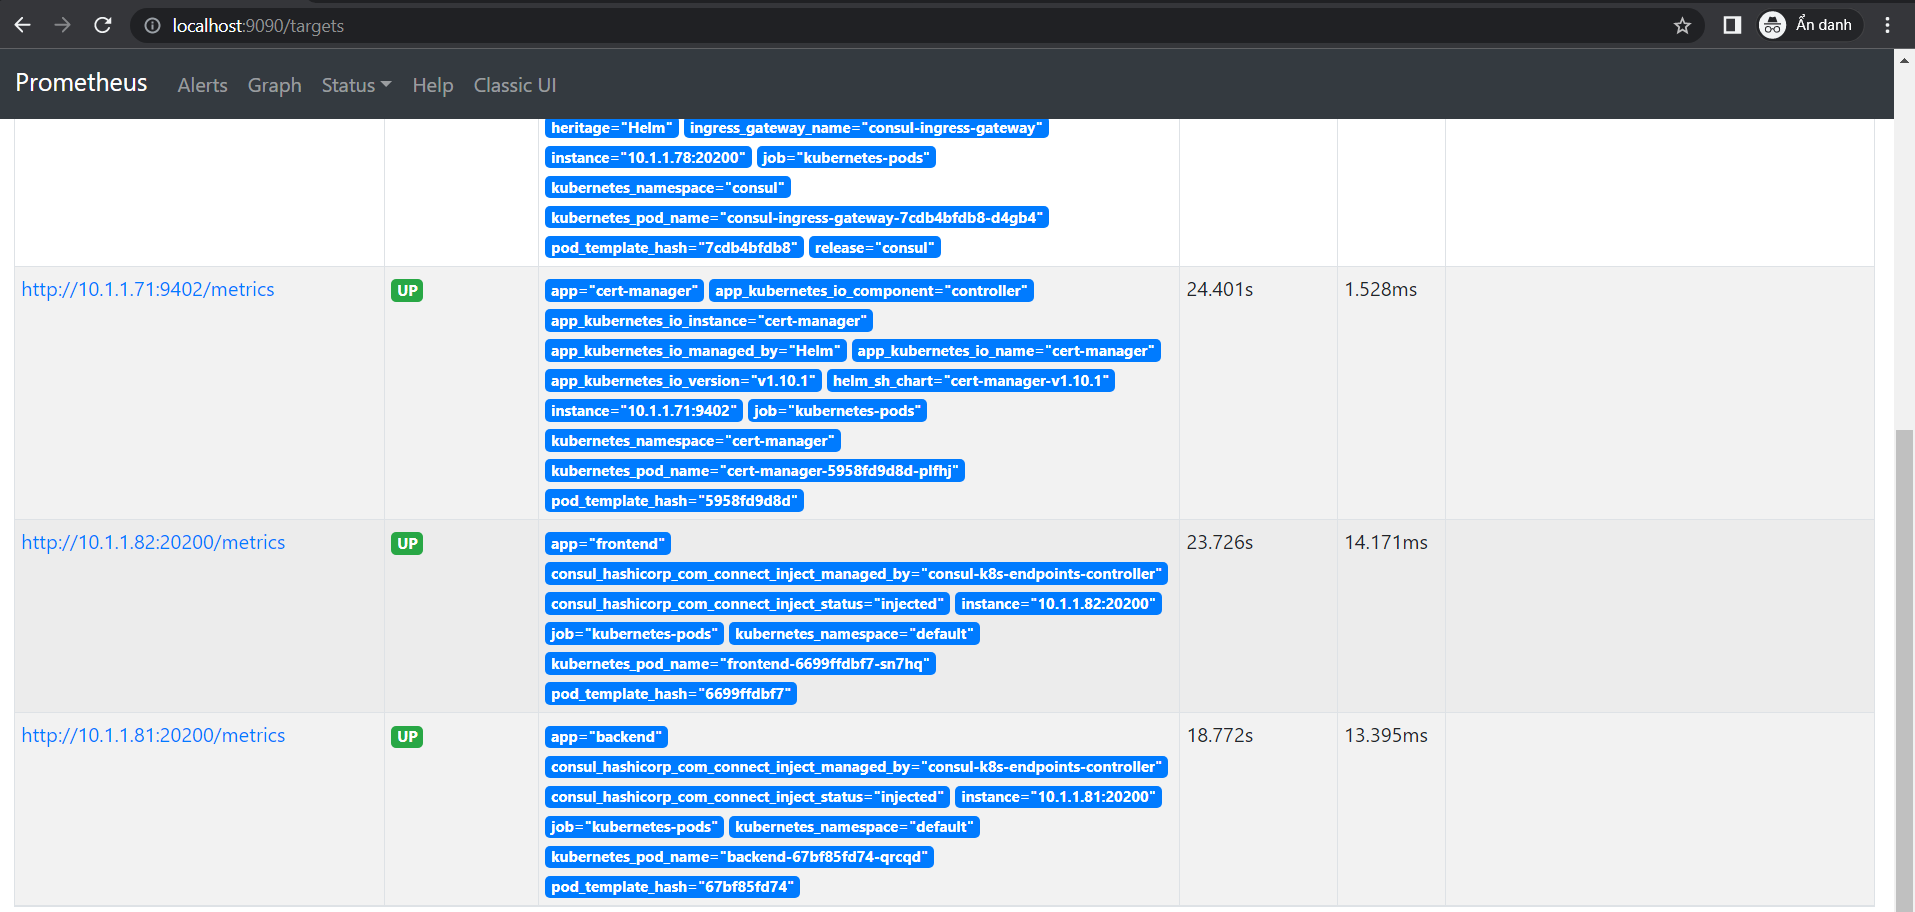
\includegraphics[width=1\linewidth]{Pics/target}
		\caption{\label{fig:target} Mục tiêu mà Prometheus đã thu thập được các metric.}
		\label{fig:target}
	\end{figure}
	\hspace{0.3cm}{Vậy là chúng ta đã đẩy được metrics lên trên Prometheus. Tiếp theo, chúng ta sẽ kiểm tra các metrics được hiện ở UI của Consul.}
	\begin{figure}[h]
	\centering
	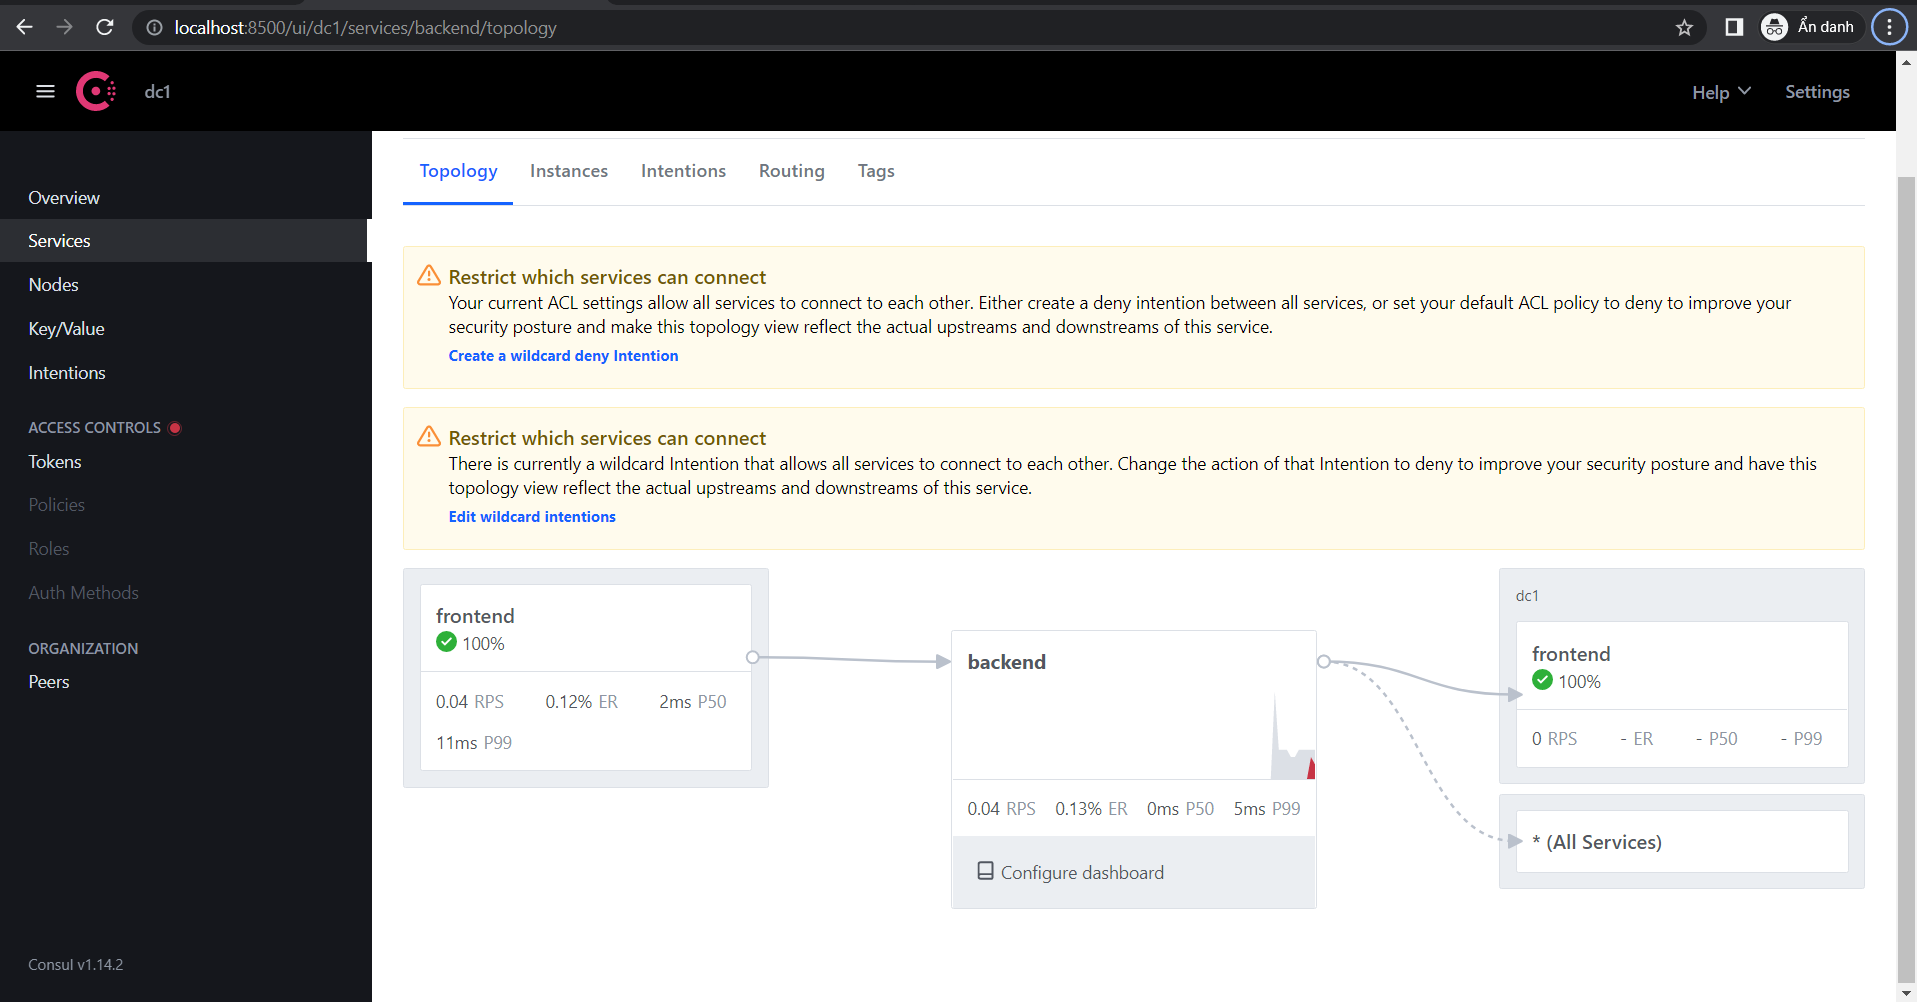
\includegraphics[width=1\linewidth]{Pics/ui-metrics}
	\caption{\label{fig:ui-metrics} Metrics hiện trên UI của Consul.}
	\label{fig:ui-metrics}
	\end{figure}
	\hspace{0.3cm}{Như vậy, chỉ việc nhìn vào cấu trúc hướng đi của các dịch vụ, chúng ta có thể nhìn thấy được các thông tin cụ thể mà metrics cung cấp trên màn hình. Điều này sẽ giúp cho việc kiểm tra và đánh giá tổng quát một cách nhanh nhất khi chúng ta có nhiều service được triển khai trên Kubernetes. \\}
	\hspace{0.3cm}{Tuy nhiên, khi mà dịch vụ không thể truy cập được, để điều tra nguyên nhân, chúng ta cần phải có một vài công cụ cụ thể hơn để có thể điều ra rõ nguồn gốc vấn đề. Để làm điều này, chúng ta sẽ triển khai thêm Jaeger, Jaeger là một công cụ giúp chúng ta điều tra cụ thể các luồng đi của dữ liệu. Để triển khai Jaeger, trước hết chúng ta cần cài đặt cert manager. Cert manager là một trong những điều kiện tiên quyết để cài đặt Jaeger. Để cài đặt Cert Manager, chúng ta cần chạy các lệnh sau:}
	\begin{lstlisting}[language=Bash]
	$ helm repo add jetstack https://charts.jetstack.io
	
	$ helm repo update
	
	$ kubectl apply -f https://github.com/cert-manager/cert-manager/releases/download/v1.10.1/cert-manager.crds.yaml
	
	$ helm install \
	cert-manager jetstack/cert-manager \
	--namespace cert-manager \
	--create-namespace \
	--version v1.10.1 \
	# --set installCRDs=true
	\end{lstlisting}
	\hspace{1.0cm}{Sau khi chạy thành công, Cert Manager đã được triển khai thành công trên kubernetes. Để kiểm tra, chúng ta sử dụng câu lệnh sau:}
	\begin{lstlisting}[language=Bash]
	$ kubectl get all -n cert-manager
	NAME                                           READY   STATUS    RESTARTS       AGE
	pod/cert-manager-5958fd9d8d-plfhj              1/1     Running   2 (3h1m ago)   2d22h
	pod/cert-manager-cainjector-7999df5dbc-h5kfl   1/1     Running   4 (3h ago)     2d22h
	pod/cert-manager-webhook-7f8f79d49c-qzkmk      1/1     Running   3 (3h1m ago)   2d22h
	
	NAME                           TYPE        CLUSTER-IP     EXTERNAL-IP   PORT(S)    AGE
	service/cert-manager           ClusterIP   10.103.15.91   <none>        9402/TCP   2d22h
	service/cert-manager-webhook   ClusterIP   10.111.32.49   <none>        443/TCP    2d22h
	
	NAME                                      READY   UP-TO-DATE   AVAILABLE   AGE
	deployment.apps/cert-manager              1/1     1            1           2d22h
	deployment.apps/cert-manager-cainjector   1/1     1            1           2d22h
	deployment.apps/cert-manager-webhook      1/1     1            1           2d22h
	
	NAME                                                 DESIRED   CURRENT   READY   AGE
	replicaset.apps/cert-manager-5958fd9d8d              1         1         1       2d22h
	replicaset.apps/cert-manager-cainjector-7999df5dbc   1         1         1       2d22h
	replicaset.apps/cert-manager-webhook-7f8f79d49c      1         1         1       2d22h
	\end{lstlisting}
	\hspace{1.0cm}{Tiếp theo đấy, chúng ta bắt đầu triển khai Jaeger. Để triển khai Jaeger, chúng ta cần chạy câu lệnh sau:}
	\begin{lstlisting}[language=Bash]
	$ kubectl create namespace observability
	$ kubectl apply -f https://github.com/jaegertracing/jaeger-operator/releases/download/v1.40.0/jaeger-operator.yaml
	customresourcedefinition.apiextensions.k8s.io/jaegers.jaegertracing.io created
	serviceaccount/jaeger-operator created
	role.rbac.authorization.k8s.io/leader-election-role created
	role.rbac.authorization.k8s.io/prometheus created
	clusterrole.rbac.authorization.k8s.io/jaeger-operator-metrics-reader created
	clusterrole.rbac.authorization.k8s.io/manager-role created
	clusterrole.rbac.authorization.k8s.io/proxy-role created
	rolebinding.rbac.authorization.k8s.io/leader-election-rolebinding created
	rolebinding.rbac.authorization.k8s.io/prometheus created
	clusterrolebinding.rbac.authorization.k8s.io/jaeger-operator-proxy-rolebinding created
	clusterrolebinding.rbac.authorization.k8s.io/manager-rolebinding created
	service/jaeger-operator-metrics created
	service/jaeger-operator-webhook-service created
	deployment.apps/jaeger-operator created
	certificate.cert-manager.io/jaeger-operator-serving-cert created
	issuer.cert-manager.io/jaeger-operator-selfsigned-issuer created
	mutatingwebhookconfiguration.admissionregistration.k8s.io/jaeger-operator-mutating-webhook-configuration created
	validatingwebhookconfiguration.admissionregistration.k8s.io/jaeger-operator-validating-webhook-configuration created
	\end{lstlisting}
	\hspace{1.0cm}{Tiếp theo, chúng ta sẽ tạo 1 tệp tin để tạo 1 ứng dụng Jaeger, pod loại Jaeger, ứng dụng này sẽ thu thập dữ liệu được gửi lên từ ứng dụng frontend và backend. Nội dung của tệp tin như sau:}
	\begin{lstlisting}[language=Bash]
	apiVersion: jaegertracing.io/v1
	kind: Jaeger
	metadata:
		name: jaeger
	spec:
		query:
			serviceType: LoadBalancer
		ingress:
			enabled: false
	\end{lstlisting}
	\hspace{1.0cm}{Sau khi tạo xong, thì Jaeger sẽ tạo cho chúng ta một deployment và giúp chúng ta có UI để truy vấn các dữ liệu. Để truy cập được UI, chúng ta cần port-forward cổng 16686 và bắt đầu truy cập vào \textit{http://localhost:16686} để xem thông tin query.}
	\begin{figure}[h]
		\centering
		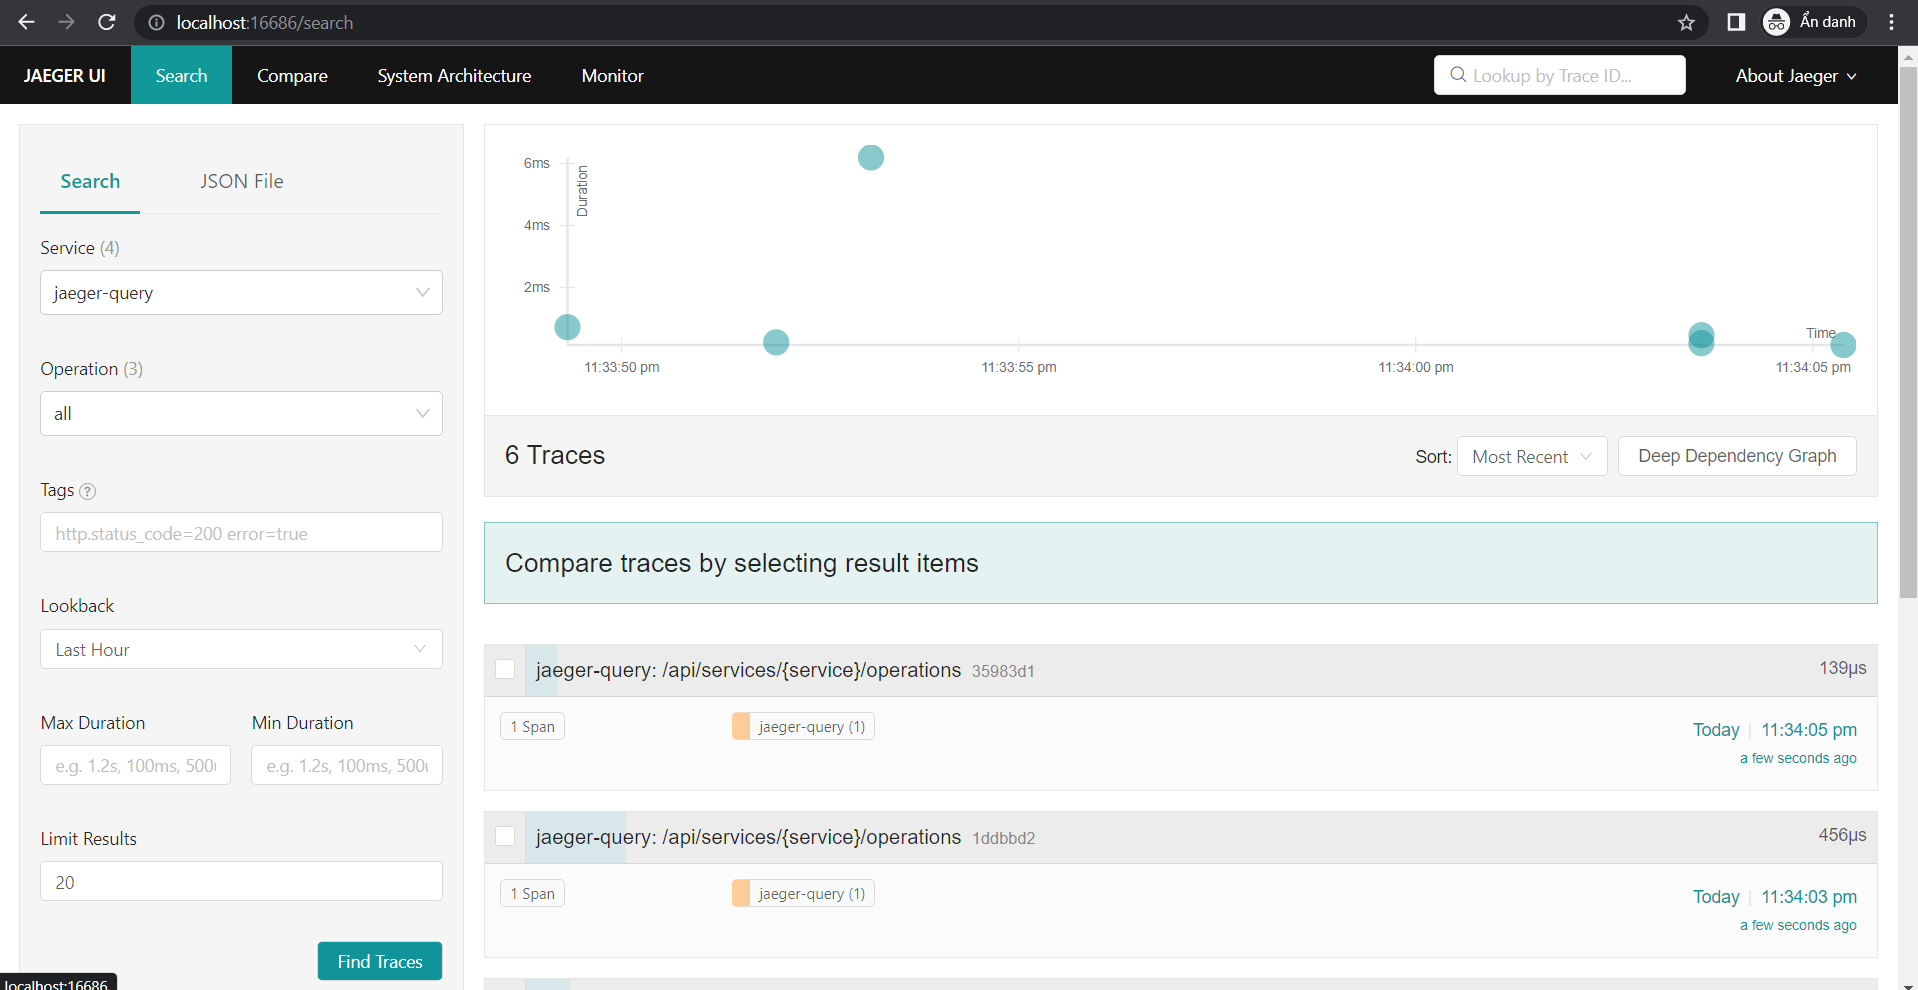
\includegraphics[width=1\linewidth]{Pics/jaeger-ui}
		\caption{\label{fig:jaeger-ui} UI của Jaeger.}
		\label{fig:jaeger-ui}
	\end{figure}
	\hspace{0.3cm}{Tiếp theo, chúng ta tiến hành đẩy dữ liệu từ ứng dụng frontend, backend và Proxy lên Jaeger. Để làm được điều này, chúng ta cần can thiệp vào trong code của ứng dụng. Tuy nhiên, ứng dụng frontend và backend đã được cấu hình để có thể đẩy dữ liệu ứng dụng lên trên Jaeger nên chúng ta chỉ việc khai báo thêm biến môi trường cho ứng dụng và ứng dụng sẽ đẩy dữ liệu lên. Còn đối với Proxy, chúng ta cần cấu hình lại một chút như sau:}
	\begin{lstlisting}[language=Bash]
	apiVersion: consul.hashicorp.com/v1alpha1
	kind: ProxyDefaults
	metadata:
		name: global
		namespace: consul
	spec:
		config:
			protocol: http
			envoy_tracing_json: |
			{
				"http":{
					"name":"envoy.tracers.zipkin",
					"typedConfig":{
						"@type":"type.googleapis.com/envoy.config.trace.v3.ZipkinConfig",
						"collector_cluster":"jaeger_collector",
						"collector_endpoint_version":"HTTP_JSON",
						"collector_endpoint":"/api/v2/spans",
						"shared_span_context":false
					}
				}
			}
			envoy_extra_static_clusters_json: |
			{
				"connect_timeout":"3.000s",
				"dns_lookup_family":"V4_ONLY",
				"lb_policy":"ROUND_ROBIN",
				"load_assignment":{
					"cluster_name":"jaeger_collector",
					"endpoints":[
					{
						"lb_endpoints":[
						{
							"endpoint":{
								"address":{
									"socket_address":{
										"address":"jaeger-collector.default",
										"port_value":9411,
										"protocol":"TCP"
									}
								}
							}
						}
						]
					}
					]
				},
				"name":"jaeger_collector",
				"type":"STRICT_DNS"
			}
	\end{lstlisting}
	\hspace{1.0cm}{Sau khi apply lại, thì chúng ta sẽ lên giao diện của Jaeger và kiểm tra: \\}
	\begin{figure}[h]
		\centering
		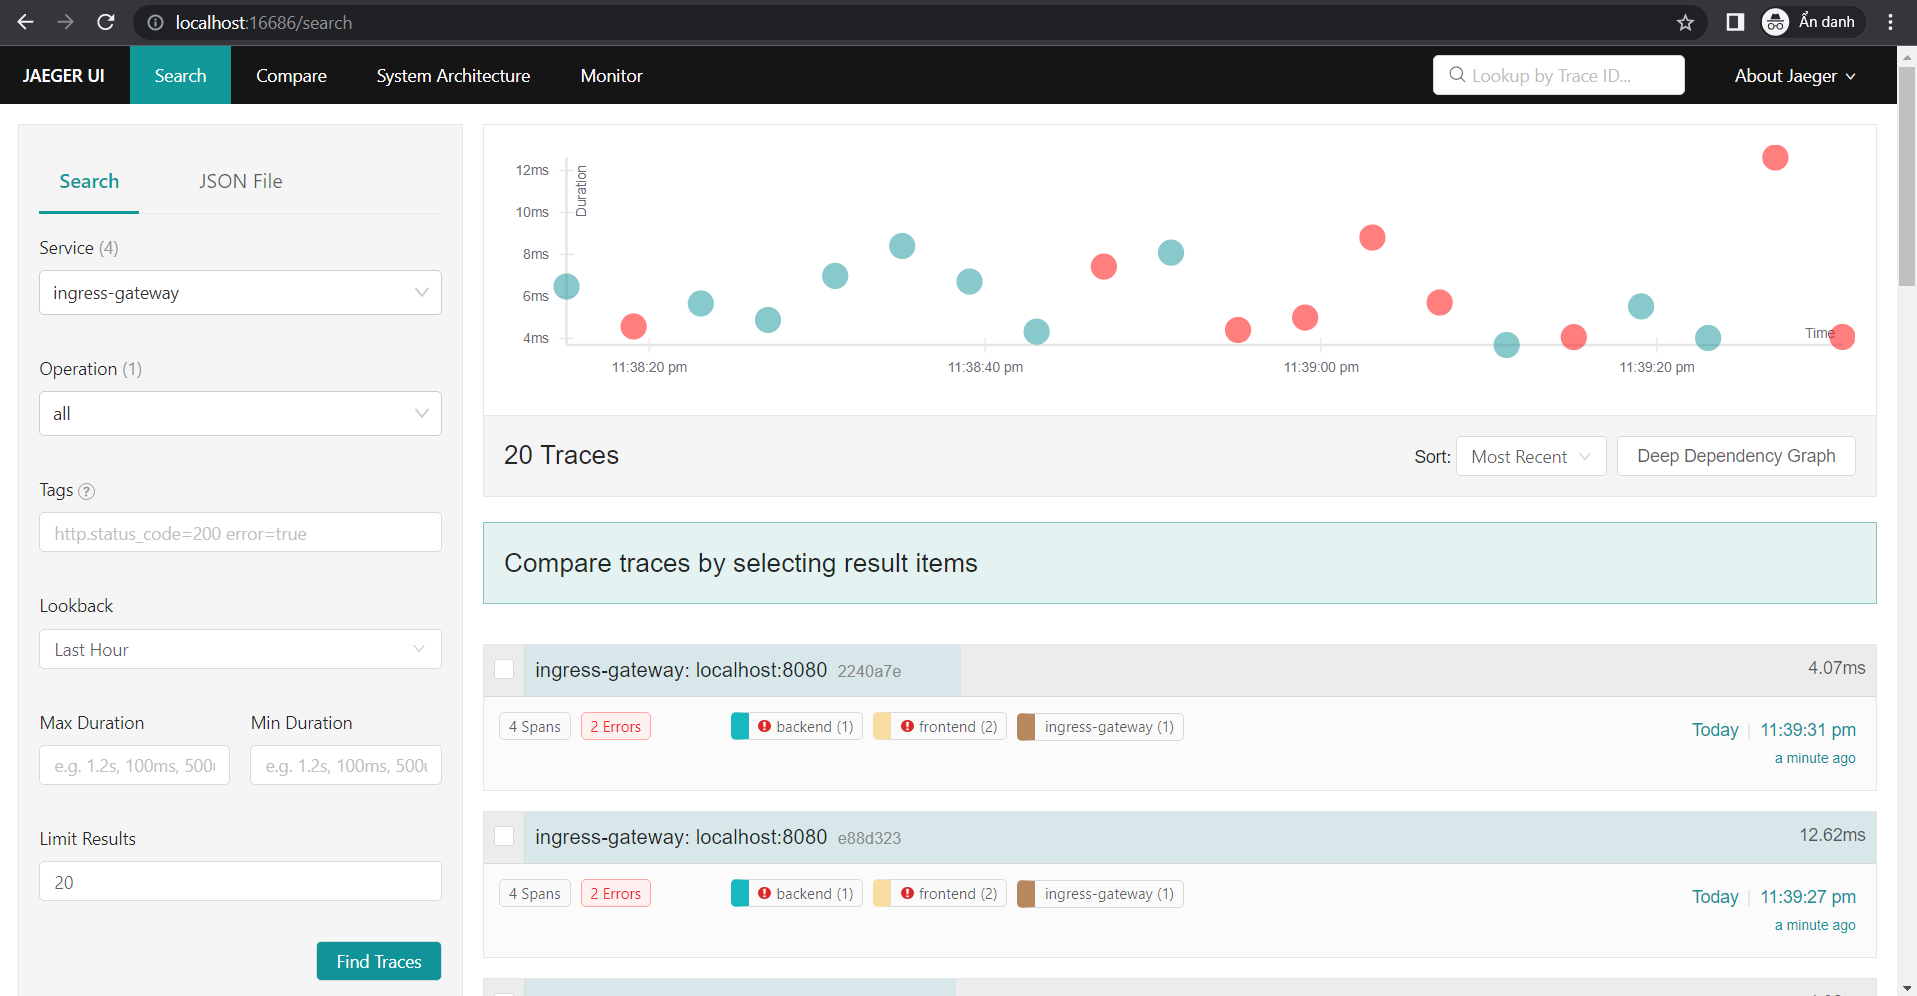
\includegraphics[width=1\linewidth]{Pics/jaeger-ingress-gateway}
		\caption{\label{fig:jaeger-ingress-gateway} Proxy đẩy dữ liệu lên Jaeger.}
		\label{fig:jaeger-ingress-gateway}
	\end{figure}
	\hspace{0.3cm}{Để điều tra, chúng ta sẽ ấn vào từng truy vấn cụ thể, và qua đấy, chúng ta sẽ biết được rằng nguyên nhân nào gây ra lỗi của ứng dụng.\\}
	\pagebreak
	\begin{figure}[h]
		\centering
		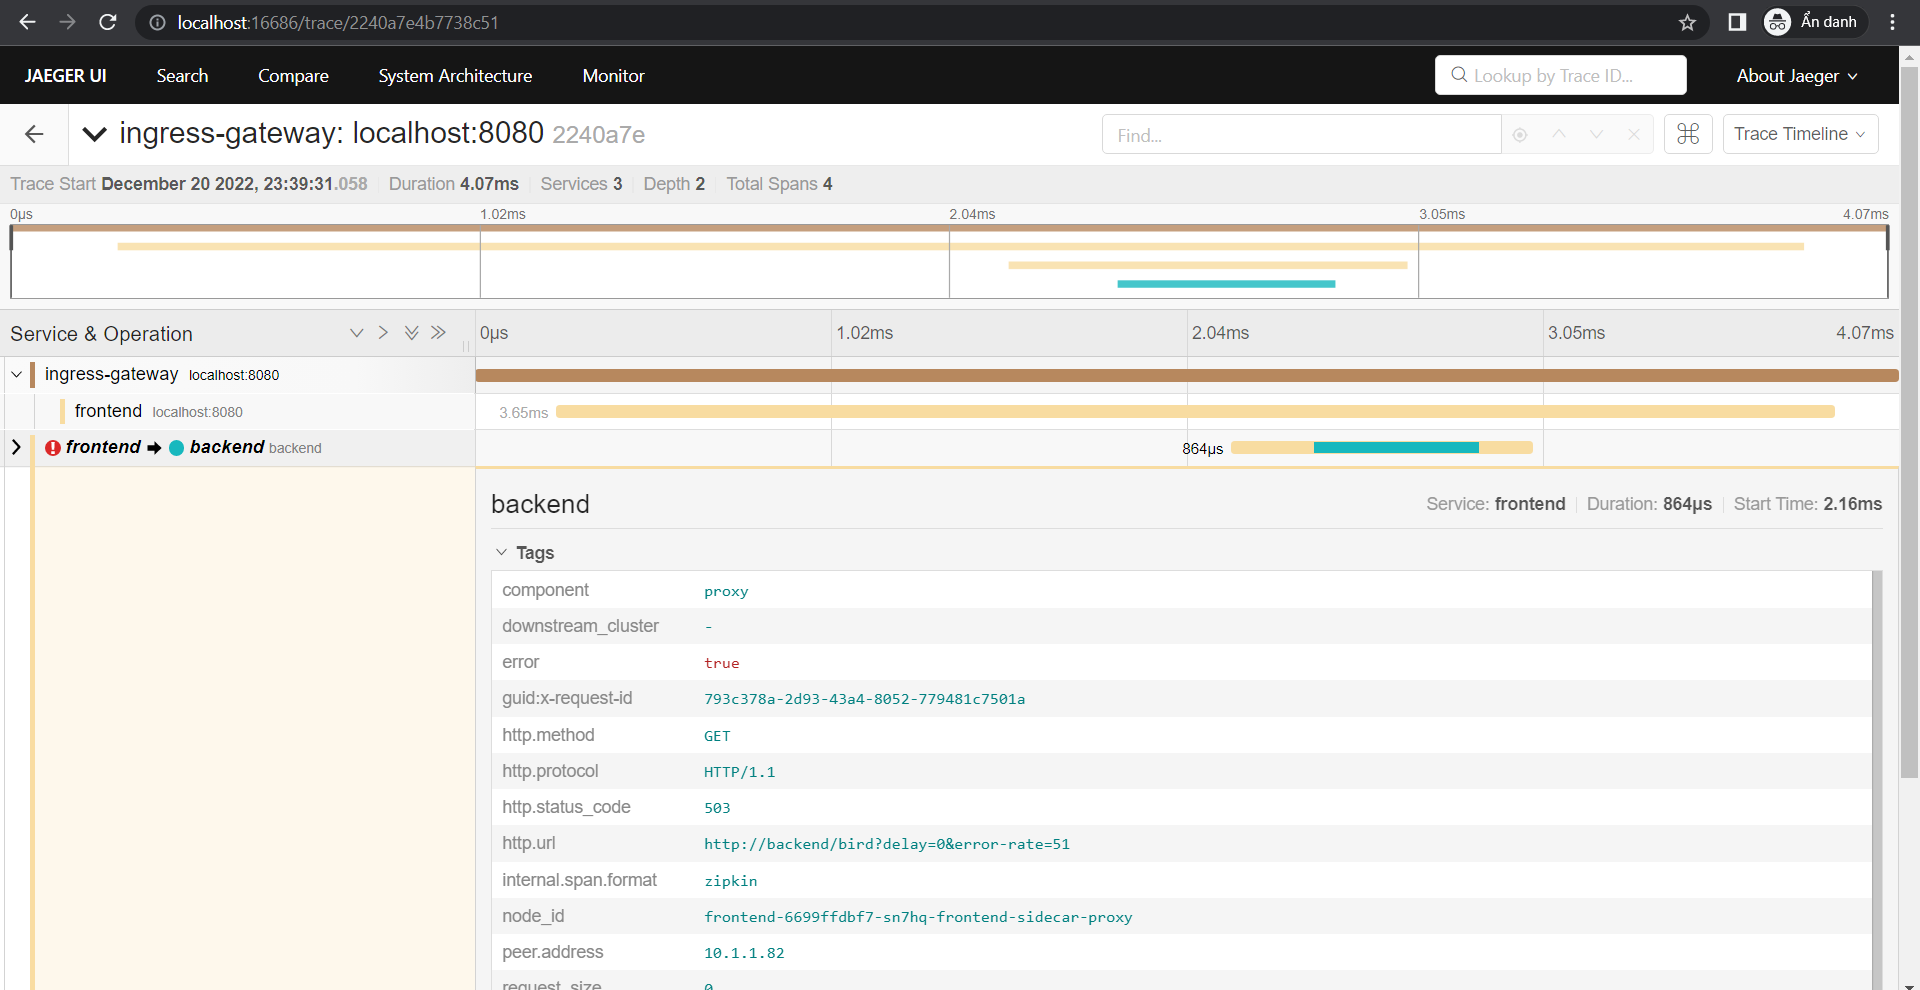
\includegraphics[width=1\linewidth]{Pics/jaeger-error}
		\caption{\label{fig:jaeger-error} Nguyên nhân lỗi đến từ backend.}
		\label{fig:jaeger-error}
	\end{figure}
	\subsubsection{Đánh giá}
	\hspace{0.3cm}{Vậy là chúng ta đã triển khai được hệ thống tracing và mở ra các metrics để có thể giúp chúng ta dễ dàng tiếp cận được những lỗi của ứng dụng. Tìm được nguyên nhân gây ra lỗi nhanh nhất có thể để làm giảm thời gian mất kết nối của hệ thống. Để triển khai phần này, thì sẽ tốn khá nhiều công sức, nhưng bù lại, khi chúng ta tìm nguyên nhân sẽ dễ dàng hơn rất nhiều vì chúng ta đã có đủ thông tin để tìm ra nguyên nhân gây ra lỗi.}
	\section{Kết luận chương 3}
	\hspace{1.0cm}{Qua chương 3, chúng ta đã thực hiện các phần thực nghiệm Consul trên Kubernetes. Qua các phần thực nghiệm này, chúng ta sẽ hiểu hơn về Consul hoạt động ra sao, vận hành như thế nào để giúp chúng ta có thể triển khai lên một cách chuẩn xác nhất và nhanh gọn nhất. Tuy nhiên, Consul vẫn nhiều tính năng mà chúng ta chưa triển khai vì phần này chúng ta chỉ tập chung vào tính năng service mesh trong consul. Vì vậy trong tương lai, chúng ta có thể tìm hiểu thêm các tính năng khác của consul và áp dụng được vào trong hệ thống kiến trúc của chúng ta.}
	\chapter*{\centering Lời kết thúc}
	\addcontentsline{toc}{chapter}{Lời kết thúc}
	\hspace{1.0cm}{Qua phần tìm hiểu trên, chúng ta đã tìm hiểu được nguyên lý hoạt động của Mircoservice, cách thức quản trị các Microservice trong Kubernetes. Qua đó, chúng ta đã nhìn thấy được tầm quan trọng của vấn đề bảo mật của Microservice trong Kubernetes. Và thứ có thể giúp chúng ta bảo mật các Microservice mà không cần phải chỉnh sửa lại code của ứng dụng đó chính là Service Mesh. Service Mesh giúp cho người quản trị có thể quản lý các Micorservice dễ dàng hơn, tăng tốc độ điều tra khi các Microservice bị lỗi, bảo mật giao tiếp giữa các Microservice. Và công cụ giúp chúng ta triển khai Service Mesh chính là Consul. Consul mặc dù tuổi đời không lâu, nhưng nó hiện đang là một trong các công cụ giúp cho người quản trị có thể dễ dàng triển khai Service Mesh lên Kubernetes để quản trị các Microservice trong Kubernetes.\\}
	
	\hspace{0.3cm}{Qua phần thực nghiệm, chúng ta đã tìm hiểu được cách thức hoạt động của Consul cũng như cách có thể vận hành Consul một cách cơ bản nhất. Tuy nhiên, Consul vẫn còn một vài điểm yếu cần phải khắc phục như là Ingress Gateway hiện tại chưa có tích hợp các chứng chỉ từ bên thứ ba và Consul là không phải OpenSource. Vì vậy Consul hiện giờ vẫn đang là một trong ít lựa chọn trong các doanh nghiệm hiện nay.}
	\chapter*{Tài liệu kham khảo}
	\section*{Consul: Up and Running}
	\section*{Microservice Security In Action}
	\section*{https://developer.hashicorp.com/consul/docs}
	\section*{https://github.com/hashicorp/consul-k8s}
	\section*{https://github.com/consul-up/examples}
	\section*{https://www.jaegertracing.io/}

\end{document}